% 1- Corrida de basalt main sin loop closure (evalsets, determinista)
% https://mateosss.pages.freedesktop.org/-/basalt/-/jobs/99328014/artifacts/report.html
% report job: https://gitlab.freedesktop.org/mateosss/basalt/-/jobs/99328014

% 2- Corrida de basalt con loop closure y rootba (evalsets, determinista)
% https://mateosss.pages.freedesktop.org/-/basalt/-/jobs/99206856/artifacts/report.html
% report job: https://gitlab.freedesktop.org/mateosss/basalt/-/jobs/99206856

% 3- Corrida de basalt con loop closure, CQ y rootba (evalsets, determinista)
% https://mateosss.pages.freedesktop.org/-/basalt/-/jobs/99477969/artifacts/report.html
% report job: https://gitlab.freedesktop.org/mateosss/basalt/-/jobs/99477969

% 4- Corridas de basalt con loop closure y rootba. (timing-evalsets, no determinista)
% https://mateosss.pages.freedesktop.org/-/basalt/-/jobs/99392746/artifacts/report.html
% report job: https://gitlab.freedesktop.org/mateosss/basalt/-/jobs/99392746

% 5- Corridas de basalt con loop closure. Usando rootba float vs double. (timing-evalsets, determinista)
% https://mateosss.pages.freedesktop.org/-/basalt/-/jobs/99426109/artifacts/report.html
% report job: https://gitlab.freedesktop.org/mateosss/basalt/-/jobs/99426109

% 6- Corridas de basalt con loop closure y rootba (timing-evalsets, determinista)
% guardo kf_timings para las secuencias MGO12, MOO12 y MIPB08
% https://mateosss.pages.freedesktop.org/-/basalt/-/jobs/100094149/artifacts/report.html
% report job: https://gitlab.freedesktop.org/mateosss/basalt/-/jobs/100094149

% 7- Corridas de basalt con loop closure y rootba, pero sin culling (timing-evalsets, determinista)
% https://mateosss.pages.freedesktop.org/-/basalt/-/jobs/100268854/artifacts/report.html
% report job: https://gitlab.freedesktop.org/mateosss/basalt/-/jobs/100268854

En este capítulo se presentan los experimentos realizados para evaluar BasaltSLAM y el análisis
de los resultados obtenidos. Primero se buscó dimensionar el impacto de las mejoras descritas
en el Capítulo \ref{sec:method}, para lo cual se realizó un estudio de ablación que compara Basalt original
con distintas versiones del sistema que incorporan las funcionalidades del mapa. Luego se evaluó
el sistema propuesto contra ORB-SLAM3 y OKVIS2 como referencias del estado del arte. En todos estos experimentos, no solo
se evaluaron métricas de error de trayectoria, sino que también se hizo énfasis en la performance, para determinar si
el sistema propuesto cumple con las limitaciones impuestas para funcionar en tiempo real. Finalmente, se concluye con
un análisis de performance detallado, que tiene en cuenta la arquitectura del sistema propuesto y las mejoras implementadas
para utilizar una optimización de bundle adjustment basada en RootBA.

La mayor parte de los experimentos fue realizada en un servidor con un procesador Intel Core i5-13600
13th Gen con 32 GB de RAM; los restantes, en una computadora con un procesador Intel Core Ultra 9 285H
con 32 GB de RAM, indicándose explícitamente cuando corresponda.

Para llevarlos a cabo se utilizaron todas las secuencias de los siguientes conjuntos de datos creados para la evaluación
de sistemas SLAM: EuRoC, TUM-VI benchmark, y el Monado SLAM Dataset, un dataset específico de XR que representa
de manera más fiel el uso esperado del sistema. A continuación se describen sus características principales.

\section{Datasets utilizados} \label{sec:datasets}

\subsection*{EuRoC}
El dataset EuRoC (European Robotics Challenge) MAV (Micro Aerial Vehicle) es uno de
los datasets más populares y utilizados en la comunidad de robótica y visión por computadora.
Consiste en 11 secuencias grabadas en tres entornos diferentes, visibles en la Figura \ref{fig:euroc_mav_frames}: una sala de máquinas (Machine Hall) y dos salas
de laboratorio de la Escuela Politécnica de Zurich (Vicon Room 1 y 2). Cada secuencia incluye datos de ground truth con una precisión milimétrica y están
disponibles los datos de calibración tanto intrínseca como extrínseca.
Todas las secuencias fueron capturadas utilizando un helicóptero Asctec Firefly equipado con
una cámara estéreo de 752 x 480 px de resolución a 20 fps y una IMU modelo ADIS16448
a 200 Hz. Los tres entornos presentan características diferenciadas:
\begin{itemize}
    \item Machine Hall: Secuencias grabadas en una sala de máquinas equipada con maquinaria pesada, proporcionando un entorno con
desafíos de iluminación y superficies reflectantes.
    \item Vicon Room 1 y 2: Secuencias grabadas en salas de laboratorio controladas, equipadas con un sistema de captura de movimiento Vicon,
diseñadas para experimentos de robótica con condiciones bien definidas y texturas variadas.
\end{itemize}

\begin{figure}[ht]
    \centering
    \begin{subfigure}[b]{0.32\textwidth}
        \centering
        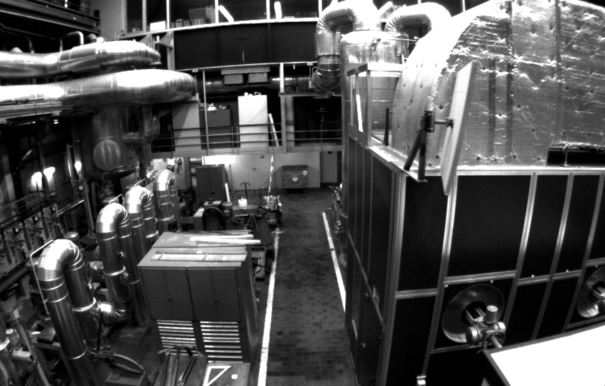
\includegraphics[width=\textwidth]{img/experiments/example_frames/MH03.png}
        \caption{Machine Hall}
        \label{fig:experiments_figure15}
    \end{subfigure}
    \hfill
    \begin{subfigure}[b]{0.32\textwidth}
        \centering
        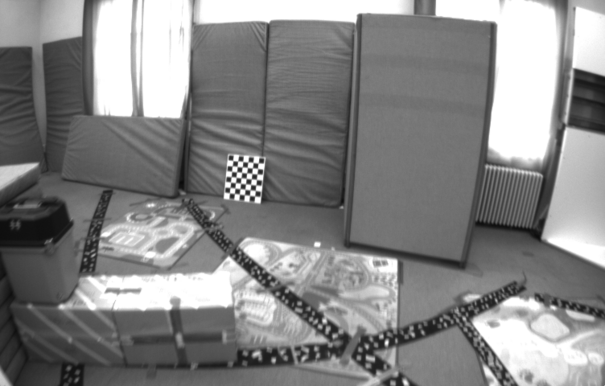
\includegraphics[width=\textwidth]{img/experiments/example_frames/V102.png}
        \caption{Vicon Room 1}
        \label{fig:experiments_figure16}
    \end{subfigure}
    \hfill
    \begin{subfigure}[b]{0.32\textwidth}
        \centering
        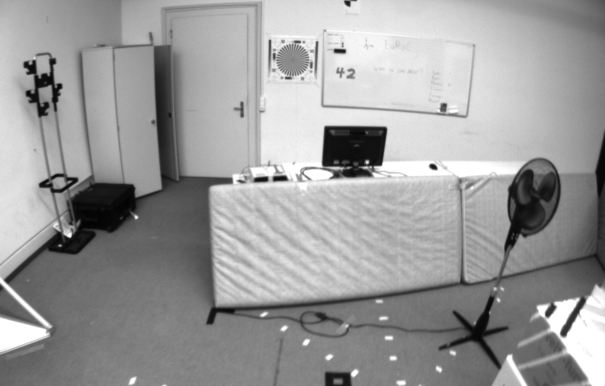
\includegraphics[width=\textwidth]{img/experiments/example_frames/V202.png}
        \caption{Vicon Room 2}
        \label{fig:experiments_figure18}
    \end{subfigure}
    \caption{Frames de ejemplo del EuRoC MAV dataset.}
    \label{fig:euroc_mav_frames}
\end{figure}

\subsection*{TUM-VI benchmark}
El TUM-VI Benchmark (Technical University of Munich Visual-Inertial Benchmark) es
otro dataset de referencia ampliamente utilizado en la comunidad de visión por computadora, ya que incluye
secuencias grabadas en diversos entornos, tanto interiores como exteriores, proporcionando un
amplio espectro de condiciones y desafíos para los sistemas de SLAM visual-inercial.

Cada secuencia fue capturada con un dispositivo sostenido manualmente (\textit{handheld}), lo cual la hace
particularmente interesante para evaluar la localización de sistemas XR. Para su captura se
utilizó una cámara estéreo de 512 x 512 px de resolución a 20 fps y una IMU de alta precisión
a 200 Hz, asegurando una correlación precisa entre los datos visuales e inerciales. Además, el
benchmark incluye trayectorias de referencia obtenidas mediante métodos de captura de mo-
vimiento, garantizando un ground truth de alta calidad para la evaluación de los
algoritmos. El dataset presenta cinco clasificaciones de secuencias, cada una con características
y desafíos únicos, visibles en la Figura \ref{fig:tum_vi_frames}:
\begin{itemize}
    \item Corridor: Secuencias en el pasillo y varias oficinas donde las poses de ground truth están disponibles para los segmentos de inicio y fin.
    \item Magistrale: Secuencias en una oficina, una gran sala y pasillos, donde las poses de ground truth están disponibles para los segmentos de inicio y fin.
    \item Outdoors: Secuencias al aire libre, donde las poses de ground truth están disponibles para los segmentos de inicio y fin.
    \item Room: Secuencias en una sala con un sistema de captura de movimiento, donde las poses de ground truth están disponibles para toda la trayectoria.
    \item Slides: Secuencias especialmente desafiantes que contienen deslizamientos en un tubo cerrado con muy mala iluminación en el interior.
    Las poses de ground truth están disponibles para los segmentos de inicio y fin.
\end{itemize}

\begin{figure}[ht]
    \centering
    \begin{subfigure}[b]{0.19\textwidth}
        \centering
        
\includegraphics[width=\textwidth]{img/experiments/example_frames/TC1.png}
        \caption{Corridor}
        \label{fig:experiments_figure15}
    \end{subfigure}
    \hfill
    \begin{subfigure}[b]{0.19\textwidth}
        \centering
        
\includegraphics[width=\textwidth]{img/experiments/example_frames/TM1.png}
        \caption{Magistrale}
        \label{fig:experiments_figure16}
    \end{subfigure}
    \hfill
    \begin{subfigure}[b]{0.19\textwidth}
        \centering
        
\includegraphics[width=\textwidth]{img/experiments/example_frames/TO2.png}
        \caption{Outdoors}
        \label{fig:experiments_figure18}
    \end{subfigure}
    \hfill
    \begin{subfigure}[b]{0.19\textwidth}
        \centering
        
\includegraphics[width=\textwidth]{img/experiments/example_frames/TR4.png}
        \caption{Room}
        \label{fig:experiments_figure20}
    \end{subfigure}
    \hfill
    \begin{subfigure}[b]{0.19\textwidth}
        \centering
        
\includegraphics[width=\textwidth]{img/experiments/example_frames/TS1.png}
        \caption{Slides}
        \label{fig:experiments_figure19}
    \end{subfigure}
    \caption{Frames de ejemplo del TUM-VI benchmark dataset.}
    \label{fig:tum_vi_frames}
\end{figure}

\subsection*{Monado SLAM Dataset}

El Monado SLAM Dataset (MSD) es un dataset visual-inercial de licencia permisiva creado
específicamente para el caso de uso de aplicaciones XR. Incluye varios tipos
de secuencias, desde juegos de VR hasta escenarios de inspección y mapeo de una habitación,
proporcionando una amplia variedad de datos para evaluar algoritmos de SLAM en contextos
de XR. El dataset contiene un ground truth con una precisión de 1 cm,
capturado mediante un sistema de tres sensores externos lighthouses.
Cuenta con 64 secuencias, con un total de 5 horas y 15 minutos de grabación en escenarios del mundo real,
incluyendo secuencias largas e ininterrumpidas de hasta 40 minutos y secuencias de juego de ritmo rápido.

Todas las secuencias son capturadas por una persona utilizando diferentes cascos XR de uso comercial para aumentar
la diversidad de los datos, como se puede ver en la Figura \ref{fig:headsets}: un Valve Index, un HP Reverb G2 y un Samsung Odyssey+.

\begin{figure}[ht]
    \centering
    \begin{subfigure}[b]{0.32\textwidth}
        \centering
        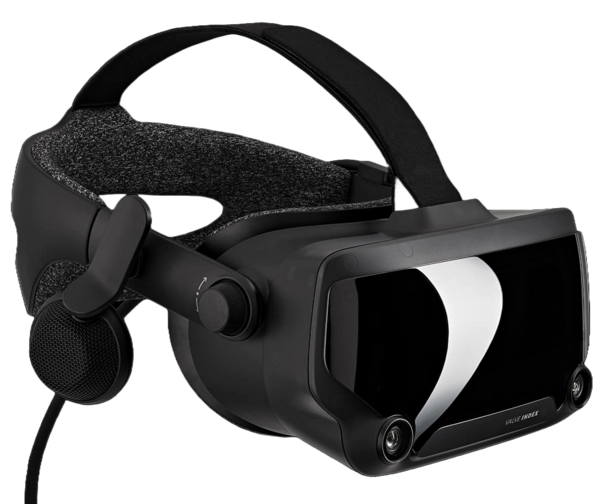
\includegraphics[width=\textwidth]{img/experiments/headset.VI.png}
        \caption{Valve Index}
        \label{fig:valve_index_headset}
    \end{subfigure}
    \hfill
    \begin{subfigure}[b]{0.32\textwidth}
        \centering
        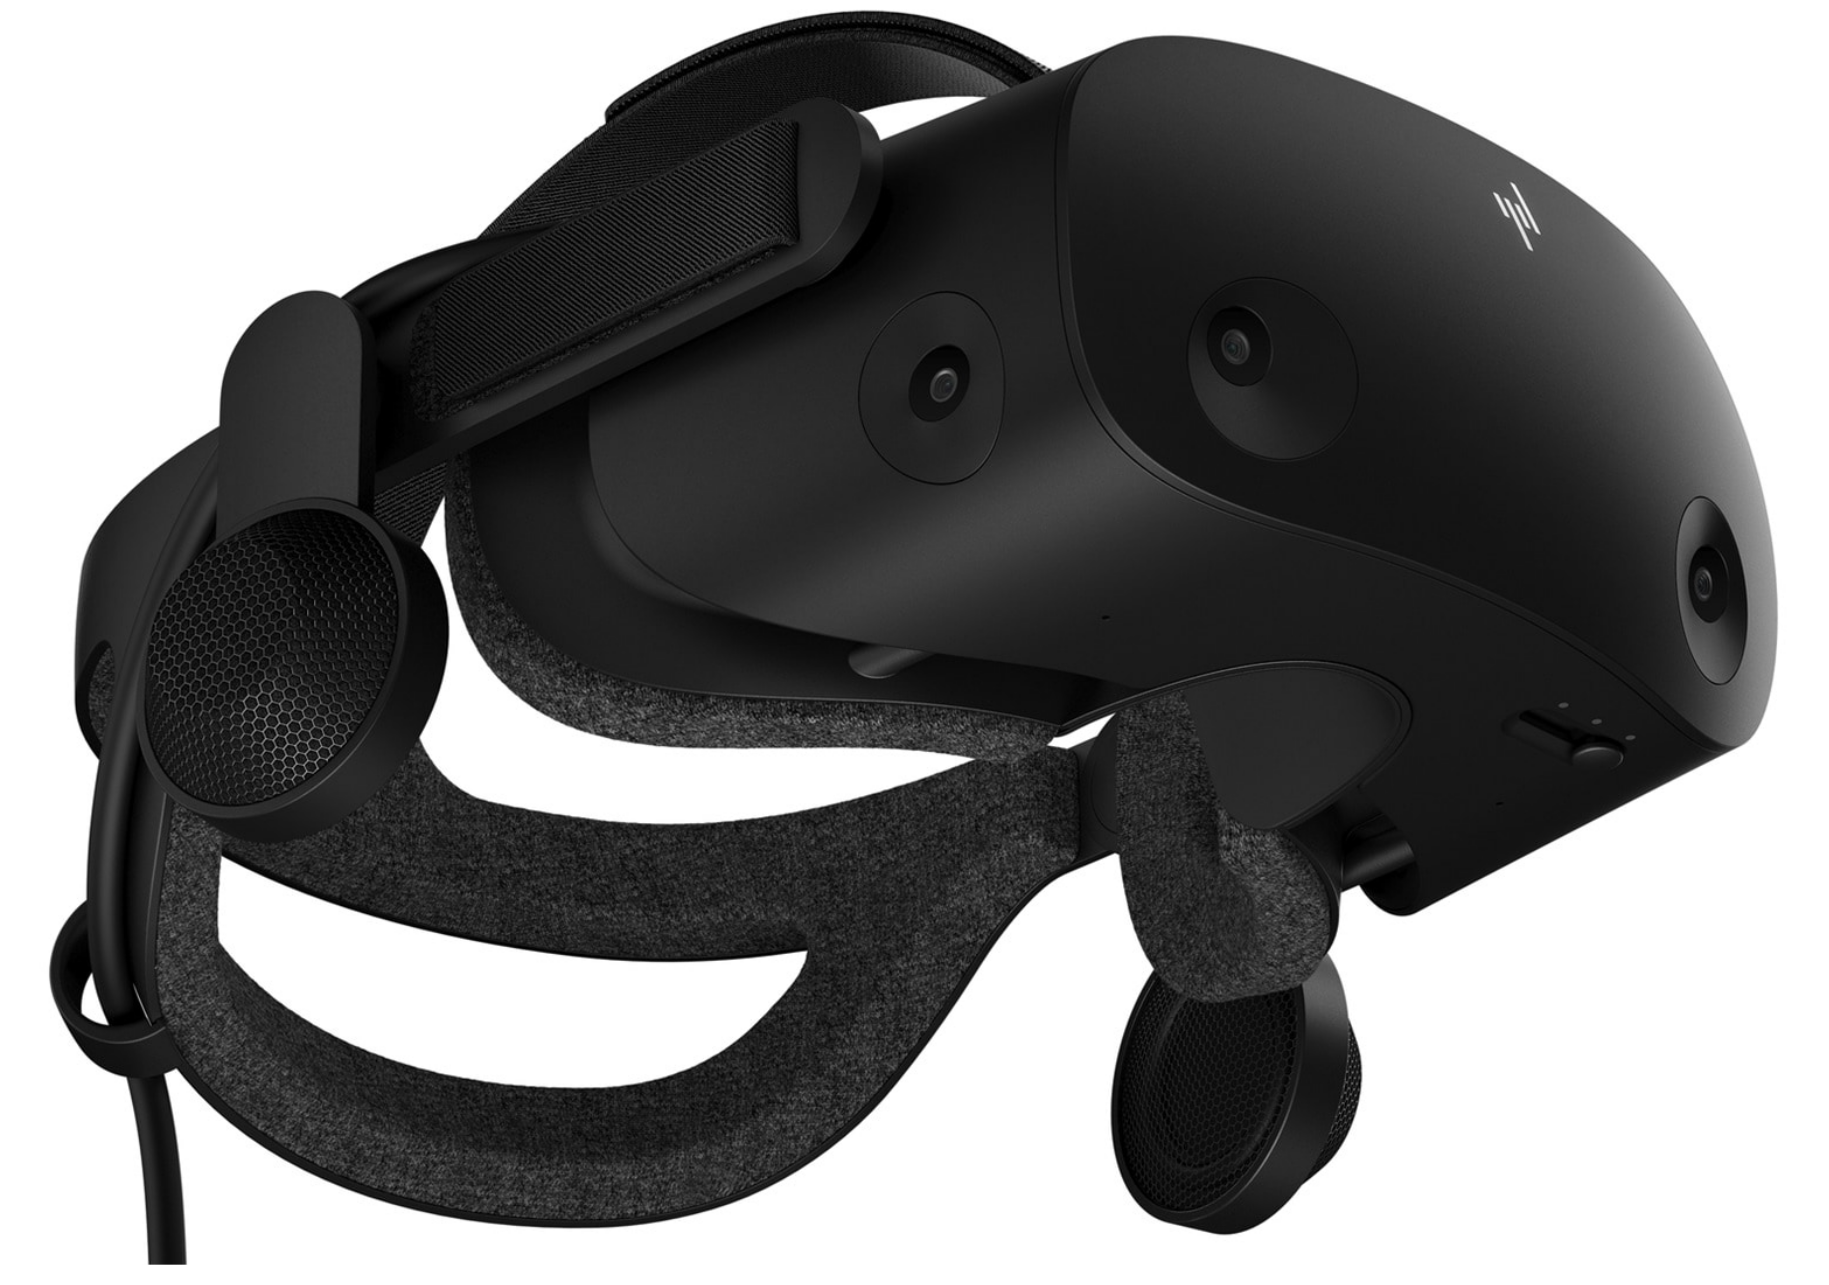
\includegraphics[width=\textwidth]{img/experiments/headset.RG2V2.png}
        \caption{HP Reverb G2}
        \label{fig:hp_reverb_g2_headset}
    \end{subfigure}
    \hfill
    \begin{subfigure}[b]{0.32\textwidth}
        \centering
        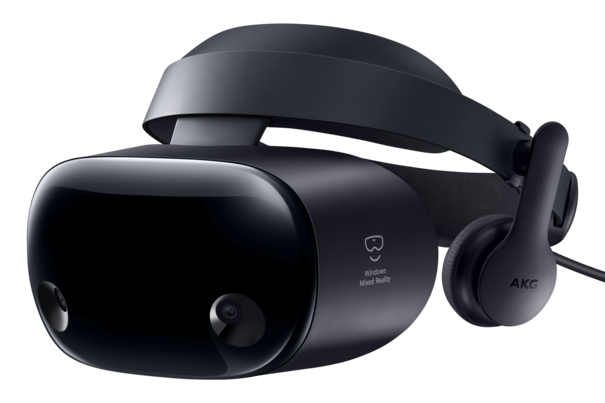
\includegraphics[width=\textwidth]{img/experiments/headset.OPlus.png}
        \caption{Samsung Odyssey+}
        \label{fig:samsung_odyssey_plus_headset}
    \end{subfigure}
    \caption{Headsets utilizados en el Monado SLAM Dataset.}
    \label{fig:headsets}
\end{figure}

Las secuencias se clasifican de la siguiente manera:
\begin{itemize}
    \item MI*: Conjunto de secuencias grabadas con el casco Valve Index que cuenta con dos cámaras
con resolución 960 x 960 px a 54 fps y una IMU a 1000 Hz. Las secuencias
MIO* incluyen diferentes escenarios como simulaciones de juegos, escaneo/mapeo de una
habitación y algunos objetos o personas en movimiento en el entorno. Las secuencias MIP*
son casos donde el usuario se encuentra jugando diferentes juegos XR, como por ejemplo Beat Saber
en SteamVR (ver Figura \ref{fig:msdmi_frame}).
    \item MO*: Conjunto de secuencias grabadas con el casco Odyssey+ el cual tiene dos cámaras con
resolución 640 x 480 px a 30 fps y una IMU a 250 Hz (ver Figura \ref{fig:msdmo_frame}).
    \item MG*: Conjunto de secuencias grabadas con el casco Reverb G2 V2 el cual tiene cuatro
cámaras con resolución 640 x 480 px a 30 fps y una IMU a 512 Hz (ver Figura \ref{fig:msdmg_frame}).
\end{itemize}

\begin{figure}[h]
    \centering
    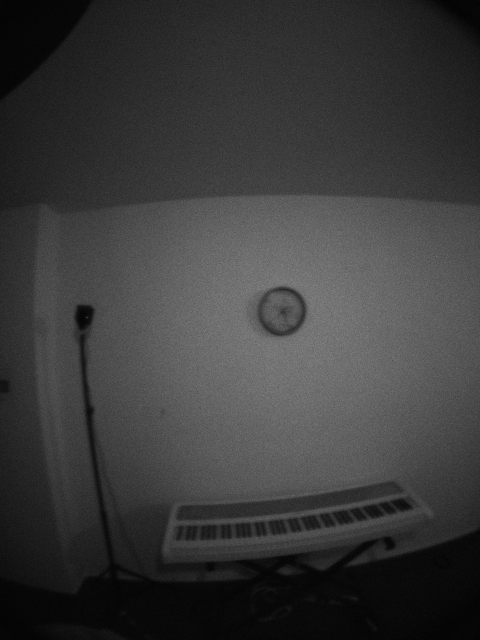
\includegraphics[width=0.24\linewidth]{img/experiments/example_frames/MGO04.1.png}
    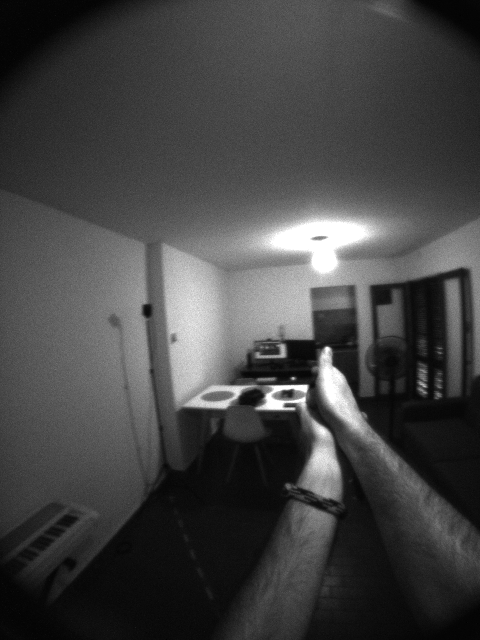
\includegraphics[width=0.24\linewidth]{img/experiments/example_frames/MGO04.2.png}
    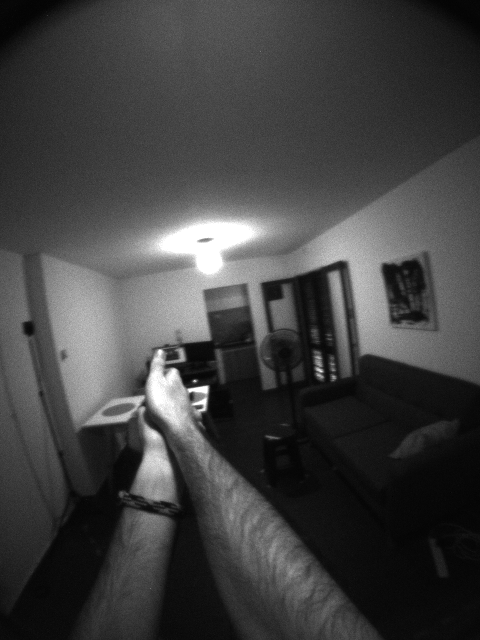
\includegraphics[width=0.24\linewidth]{img/experiments/example_frames/MGO04.3.png}
    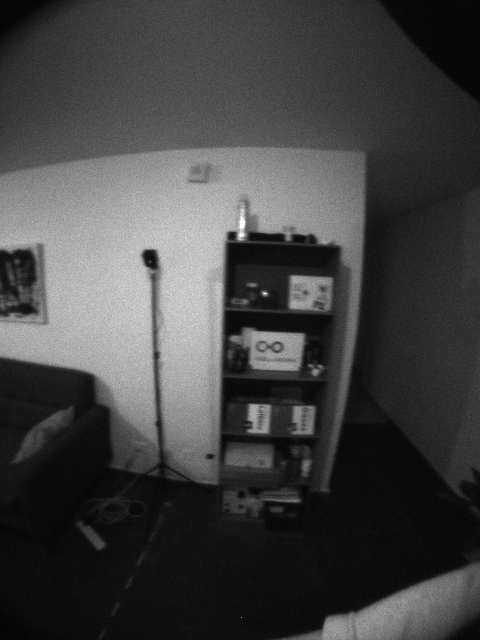
\includegraphics[width=0.24\linewidth]{img/experiments/example_frames/MGO04.4.png}
    \caption{Frame de ejemplo de la secuencia MGO04 (Reverb G2 V2).}
    \label{fig:msdmg_frame}
\end{figure}

\begin{figure}[h]
    \centering
    
\includegraphics[width=0.48\linewidth]{img/experiments/example_frames/MOO08.1.png}
    
\includegraphics[width=0.48\linewidth]{img/experiments/example_frames/MOO08.2.png}
    \caption{Frame de ejemplo de la secuencia MOO08 (Odyssey+).}
    \label{fig:msdmo_frame}
\end{figure}

\begin{figure}[h]
    \centering
    
\includegraphics[width=0.48\linewidth]{img/experiments/example_frames/MIPT02.1.png}
    
\includegraphics[width=0.48\linewidth]{img/experiments/example_frames/MIPT02.2.png}
    \caption{Frame de ejemplo de la secuencia MIPT02 (Valve Index).}
    \label{fig:msdmi_frame}
\end{figure}


\section{Métricas} \label{sec:metrics}

Para evaluar los resultados de los experimentos es necesario contar con métricas que
permitan comparar la precisión y la robustez de las trayectorias estimadas por los distintos sistemas
VI-SLAM.

En este trabajo se emplean dos métricas ampliamente utilizadas en el estado del arte:
el Error de Trayectoria Absoluto (ATE, \textit{Absolute Trajectory Error}) y el Error de Trayectoria
Relativo (RTE, \textit{Relative Trajectory Error}). El ATE mide la diferencia global entre la trayectoria
estimada y la trayectoria real del sensor en el espacio, proporcionando una indicación de la
precisión absoluta del sistema a lo largo de toda la secuencia. Por otro lado, el RTE evalúa la
precisión local del sistema midiendo la discrepancia entre segmentos cortos de las trayectorias, es
decir, compara la posición relativa entre puntos cercanos en las trayectorias estimada y real. Esta
métrica es útil para analizar la consistencia del sistema en intervalos cortos de tiempo.

Además, existen dos formas de evaluar las trayectorias estimadas por los sistemas de SLAM: de manera
causal o no causal. En la primera, se evalúan las estimaciones que utilizan todas las mediciones hasta el respectivo
timestamp de cada pose, es decir, tan pronto como se estima la pose, se reporta para ser comparada con el ground truth.
En la evaluación no causal, se evalúa la trayectoria final completamente optimizada, donde se tienen en cuenta todas las
mediciones para todas las estimaciones, incluyendo las correcciones de loop closure.

En los sistemas tradicionales, en la evaluación causal el error de drift acumulado puede dominar las
estadísticas del ATE, ya que la trayectoria contiene los característicos ``saltos'' cuando se cierran ciclos.
En cambio, para el sistema implementado en este trabajo, esto no sucederá en las evaluaciones
causales, porque la pose del keyframe más reciente se mantiene fija en la optimización. Sin embargo, el error causal
no tendrá ninguna corrección de drift, y esto hará que sea exactamente igual al error de Basalt en su versión VIO.
Por estos motivos, en la totalidad de los experimentos que evalúen ATE o RTE, se optará por usar la trayectoria no causal.

Es importante notar que en el mapa se guardan solo poses de keyframes, ya que tanto la optimización de los cierres de
ciclos, como el bundle adjustment final, se realizan sobre keyframes. Con el fin de poder comparar
las trayectorias estimadas por este sistema, con las estimadas por los sistemas del estado del arte, se recuperan las poses de los frames
intermedios a través de interpolación entre los keyframes temporalmente más cercanos, tanto para el ATE como para el RTE.

% The keyframes must be a subset of the frames. They may have optimized poses, that differ from the frames' poses. For every non-keyframe frame f between optimized keyframes KF_i and KF_{i+1} its pose is recovered via two-sided interpolation:
% T_f_left  = T_KFi_opt  * T_KFi_raw.inv()  * T_f_raw
% T_f_right = T_KFi1_opt * T_KFi1_raw.inv() * T_f_raw
% T_f       = slerp/lerp(T_f_left, T_f_right, alpha)
% where alpha = (t_f - t_KFi) / (t_KFi1 - t_KFi).
%
%Se nota $f$ o $T\_w\_i$ a la pose del frame $f$ luego de optimizar el mapa (no causal). Y se nota con
%$t\_raw$ o $T\_w\_i^{raw}$ a la pose del frame $f$ antes de optimizar el mapa (causal). Luego, para todo frame $f$,
%que se encuentra entre los keyframes temporalmente más cercanos $KF_i$ y $KF_{i+1}$, se recupera su pose a través
%de interpolación bilateral.
%
%$$ T\_f\_left = T_{KF_i}^{opt} \cdot (T_{KF_i}^{raw})^{-1} \cdot T_f^{raw} $$
%$$ T\_f\_right = T_{KF_{i+1}}^{opt} \cdot (T_{KF_{i+1}}^{raw})^{-1} \cdot T_f^{raw} $$
%$$ T_f = \text{slerp/lerp}(T\_f\_left, T\_f\_right, \alpha) $$
%$$ \alpha = \frac{t_f - t_{KF_i}}{t_{KF_{i+1}} - t_{KF_i}} $$


Además de las métricas cuantitativas previas, se hará énfasis en analizar la performance de los sistemas,
para determinar si cumplen con las limitaciones de tiempo real impuestas para su uso en aplicaciones XR.
Para esto se analizará el tiempo de ejecución de cada sistema, tanto en términos de tiempo total como en
términos de tiempo por frame. De acuerdo a los tipos de cámaras previamente mencionados, los límites de
funcionamiento para tiempo real son: 18.5 ms por frame para las secuencias MI*, 33.3 ms para las secuencias
MO* y MG*, y 50 ms para las secuencias de EuRoC y TUM-VI. Para ello, es importante mencionar
los distintos modos de ejecución con los que cuenta el sistema propuesto:
\begin{itemize}
    \item Síncrono. Las operaciones se ejecutan de manera secuencial. Es decir, para cada frame primero se lo procesa en el frontend,
    luego se lo optimiza en el VIO, y luego se agrega en el mapa, detectando y cerrando ciclos si los hubiere. Una vez que
    se completa el procesamiento completo del frame, se introduce el siguiente. Este modo de ejecución sirve para facilitar
    la reproducción de resultados. Sin embargo, no es el modo de ejecución recomendado para aplicaciones XR,
    ya que no se aprovechan las ventajas de la arquitectura del sistema.
    \item Asíncrono. Las operaciones se ejecutan de manera concurrente, permitiendo que el sistema procese múltiples
    frames al mismo tiempo. En este modo, el frontend puede procesar un nuevo frame mientras el VIO optimiza la trayectoria.
    Además, el mapa recibe nuevos keyframes a medida que ingresan en el VIO, pero no bloquea a ningún otro componente mientras ejecuta
    sus operaciones como culling y loop closure.
    \item Síncrono con mapa asíncrono. En este modo, el frontend y el VIO se ejecutan de manera secuencial, pero el mapa
    de manera concurrente. Permitiendo un mayor control sobre el flujo de ejecución, sin bloquear componentes cuando el mapa
    realiza las operaciones más costosas.
\end{itemize}

\section{Estudio de ablación}

Con el fin de cuantificar el impacto individual de cada mejora implementada, se realizó
un estudio de ablación que compara Basalt original con distintas versiones del sistema,
incorporando progresivamente las funcionalidades propuestas. Las versiones evaluadas son:

\begin{itemize}
    \item Basalt: Versión original de Basalt, no mantiene un mapa persistente.
    \item BasaltLC: Versión de Basalt que mantiene un mapa persistente, detecta y cierra ciclos, y realiza keyframe culling.
    \item BasaltSLAM: Versión de Basalt que realiza las mismas operaciones que BasaltLC, pero además optimiza el mapa final con RootBA.
    \item BasaltSLAM-CQ: Versión de Basalt que realiza las mismas operaciones que BasaltSLAM. Además, durante la ejecución,
    reintroduce hasta 3 keyframes en la ventana de keyframes del VIO, basándose en el grafo de covisibilidad del mapa.
\end{itemize}

Para este experimento, se dividirán los datasets en dos categorías: “Datasets del estado del
arte” (EuRoC y TUM-VI) y “Datasets de XR” (Monado SLAM Dataset). En cada caso, se
presentarán las métricas ATE y RTE, comentadas en la Sección \ref{sec:metrics}. Se incluirá una tabla por métrica y tipo
de secuencia según las mencionadas en la Sección \ref{sec:datasets}. En caso
de que un sistema termine abruptamente o no sea capaz de estimar la trayectoria,
se utilizará un guion ('-') para indicar la falla. Al final de cada tabla se agregan las filas ``Mean'' y ``Median''
que muestran el promedio y mediana de las secuencias que corrieron correctamente.

Además, en las columnas que correspondan a versiones del sistema que detectan ciclos, se indicará entre paréntesis
la cantidad de ciclos detectados.

\subsection{Resultados en datasets del estado del arte}

En la Tabla \ref{tab:corridor_ablation_all} se muestran los resultados de ATE, RTE y cantidad de ciclos detectados en las secuencias de ``Corridor''.
Se observa una mejora significativa en ambas métricas, a excepción de la secuencia TC4, donde el sistema no detectó ningún ciclo
y por ende no se produjo ninguna mejora.

\begin{table}[ht]
\centering
\caption{ATE [cm], RTE [cm] y ciclos detectados en TUM-VI Corridor.}
\label{tab:corridor_ablation_all}
\begin{tabular}{l rrrr | rrrr | rrrr}
\toprule
& \multicolumn{4}{c|}{\textbf{ATE [cm]}} & \multicolumn{4}{c|}{\textbf{RTE [cm]}} & \multicolumn{4}{c}{\textbf{Ciclos}} \\
\cmidrule(lr){2-5} \cmidrule(lr){6-9} \cmidrule(lr){10-13}
\textbf{Secuencia}
& \rotatebox{90}{\textbf{Basalt}\,}
& \rotatebox{90}{\textbf{BasaltLC}\,}
& \rotatebox{90}{\textbf{BasaltSLAM}\,}
& \rotatebox{90}{\textbf{BasaltSLAM-CQ}\,}
& \rotatebox{90}{\textbf{Basalt}\,}
& \rotatebox{90}{\textbf{BasaltLC}\,}
& \rotatebox{90}{\textbf{BasaltSLAM}\,}
& \rotatebox{90}{\textbf{BasaltSLAM-CQ}\,}
& \rotatebox{90}{\textbf{Basalt}\,}
& \rotatebox{90}{\textbf{BasaltLC}\,}
& \rotatebox{90}{\textbf{BasaltSLAM}\,}
& \rotatebox{90}{\textbf{BasaltSLAM-CQ}\,} \\
\midrule
TC1 & 32.1 & 6.8 & 2.8 & \textbf{1.3} & 6.3 & 5.9 & 5.5 & \textbf{0.5} & -- & 16 & 16 & 11 \\
TC2 & 44.4 & 8.8 & \textbf{7.2} & 11.4 & 7.4 & 1.8 & \textbf{1.4} & 1.5 & -- & 13 & 13 & 14 \\
TC3 & 61.3 & 5.0 & 6.4 & \textbf{4.6} & 9.6 & 3.5 & 3.1 & \textbf{0.9} & -- & 19 & 19 & 9 \\
TC4 & 22.3 & 22.3 & \textbf{22.0} & 26.4 & 3.7 & 3.7 & \textbf{3.6} & 4.4 & -- & 0 & 0 & 0 \\
TC5 & 36.2 & 11.4 & \textbf{3.1} & 4.4 & 10.1 & 3.2 & \textbf{0.7} & 1.4 & -- & 9 & 9 & 6 \\
\midrule
Mediana & 36.2 & 8.8 & 6.4 & \textbf{4.6} & 7.4 & 3.5 & 3.1 & \textbf{1.4} & -- & -- & -- & -- \\
Promedio & 39.2 & 10.9 & \textbf{8.3} & 9.6 & 7.4 & 3.6 & 2.8 & \textbf{1.7} & -- & -- & -- & -- \\
\bottomrule
\end{tabular}
\end{table}

En la Tabla \ref{tab:magistrale_ablation_all} se muestran los resultados de ATE, RTE y ciclos detectados en las secuencias de ``Magistrale''.
Si bien en todas las secuencias los sistemas SLAM logran una mejora respecto a Basalt, principalmente en ATE, dicha mejora es especialmente notable en
TM1 y TM6, donde BasaltSLAM es capaz de corregir drifts acumulados de más de 3 metros.
En todas las secuencias se detectaron ciclos; sin embargo, como se puede observar en la Figura \ref{fig:loops_tm1}, uno de los ciclos de TM1 fue detectado
entre keyframes temporalmente distantes, lo cual hace que la corrección de drift sea más efectiva. Lo mismo ocurre
en TM6, a diferencia de las demás secuencias.

\begin{table}[ht]
\centering
\caption{ATE [cm], RTE [cm] y ciclos detectados en TUM-VI Magistrale.}
\label{tab:magistrale_ablation_all}
\begin{tabular}{l rrrr | rrrr | rrrr}
\toprule
& \multicolumn{4}{c|}{\textbf{ATE [cm]}} & \multicolumn{4}{c|}{\textbf{RTE [cm]}} & \multicolumn{4}{c}{\textbf{Ciclos}} \\
\cmidrule(lr){2-5} \cmidrule(lr){6-9} \cmidrule(lr){10-13}
\textbf{Secuencia}
& \rotatebox{90}{\textbf{Basalt}\,}
& \rotatebox{90}{\textbf{BasaltLC}\,}
& \rotatebox{90}{\textbf{BasaltSLAM}\,}
& \rotatebox{90}{\textbf{BasaltSLAM-CQ}\,}
& \rotatebox{90}{\textbf{Basalt}\,}
& \rotatebox{90}{\textbf{BasaltLC}\,}
& \rotatebox{90}{\textbf{BasaltSLAM}\,}
& \rotatebox{90}{\textbf{BasaltSLAM-CQ}\,}
& \rotatebox{90}{\textbf{Basalt}\,}
& \rotatebox{90}{\textbf{BasaltLC}\,}
& \rotatebox{90}{\textbf{BasaltSLAM}\,}
& \rotatebox{90}{\textbf{BasaltSLAM-CQ}\,} \\
\midrule
TM1 & 182.9 & 8.6 & \textbf{7.4} & 14.9 & 20.3 & 1.5 & \textbf{1.2} & 2.0 & -- & 69 & 69 & 42 \\
TM2 & 150.2 & 100.6 & 87.3 & \textbf{80.4} & 17.0 & 12.0 & 10.2 & \textbf{9.5} & -- & 16 & 16 & 15 \\
TM3 & 197.1 & 166.3 & \textbf{166.2} & 243.3 & 23.4 & \textbf{20.1} & 20.2 & 27.7 & -- & 6 & 6 & 3 \\
TM4 & 151.1 & 156.9 & \textbf{150.8} & 199.9 & \textbf{14.4} & 15.8 & 14.7 & 18.3 & -- & 16 & 16 & 8 \\
TM5 & 100.5 & 95.8 & \textbf{95.0} & 188.9 & 11.5 & 10.8 & \textbf{10.5} & 21.3 & -- & 2 & 2 & 2 \\
TM6 & 320.1 & 3.0 & \textbf{1.7} & 32.2 & 48.7 & 1.6 & \textbf{1.1} & 5.8 & -- & 12 & 12 & 12 \\
\midrule
Mediana & 167.0 & 98.2 & \textbf{91.1} & 134.7 & 18.7 & 11.4 & \textbf{10.3} & 13.9 & -- & -- & -- & -- \\
Promedio & 183.7 & 88.5 & \textbf{84.7} & 126.6 & 22.5 & 10.3 & \textbf{9.6} & 14.1 & -- & -- & -- & -- \\
\bottomrule
\end{tabular}
\end{table}

En la Tabla \ref{tab:outdoors_ablation_all} se muestran los resultados de ATE, RTE y ciclos detectados en las secuencias de ``Outdoors''.
No se observa una mejora como en las secuencias anteriores. Tan solo se observa una mejora en TO7, donde se detectaron 24 ciclos, y algunos de ellos
fueron entre keyframes que se encuentran alejados temporalmente, como se observa en la Figura \ref{fig:loops_to7}.
Sin embargo, en el resto de las secuencias, los ciclos detectados fueron entre keyframes muy cercanos
temporalmente, como se observa en las Figura \ref{fig:loops_to3}, lo cual hace que el drift acumulado durante la trayectoria en el exterior no se corrija.

\begin{table}[ht]
\centering
\caption{ATE [cm], RTE [cm] y ciclos detectados en TUM-VI Outdoors.}
\label{tab:outdoors_ablation_all}
\resizebox{\textwidth}{!}{
\begin{tabular}{l rrrr | rrrr | rrrr}
\toprule
& \multicolumn{4}{c|}{\textbf{ATE [cm]}} & \multicolumn{4}{c|}{\textbf{RTE [cm]}} & \multicolumn{4}{c}{\textbf{Ciclos}} \\
\cmidrule(lr){2-5} \cmidrule(lr){6-9} \cmidrule(lr){10-13}
\textbf{Secuencia}
& \rotatebox{90}{\textbf{Basalt}\,}
& \rotatebox{90}{\textbf{BasaltLC}\,}
& \rotatebox{90}{\textbf{BasaltSLAM}\,}
& \rotatebox{90}{\textbf{BasaltSLAM-CQ}\,}
& \rotatebox{90}{\textbf{Basalt}\,}
& \rotatebox{90}{\textbf{BasaltLC}\,}
& \rotatebox{90}{\textbf{BasaltSLAM}\,}
& \rotatebox{90}{\textbf{BasaltSLAM-CQ}\,}
& \rotatebox{90}{\textbf{Basalt}\,}
& \rotatebox{90}{\textbf{BasaltLC}\,}
& \rotatebox{90}{\textbf{BasaltSLAM}\,}
& \rotatebox{90}{\textbf{BasaltSLAM-CQ}\,} \\
\midrule
TO1 & 27481.9 & 28421.9 & 28423.9 & \textbf{26650.7} & 2820.4 & 2919.3 & 2918.2 & \textbf{2737.7} & -- & 5 & 5 & 3 \\
TO2 & \textbf{5851.7} & 6042.3 & 6045.3 & 7545.5 & \textbf{629.4} & 647.4 & 647.1 & 808.4 & -- & 18 & 18 & 5 \\
TO3 & \textbf{3387.7} & 3488.7 & 3492.5 & 3504.2 & \textbf{340.2} & 349.6 & 349.7 & 350.1 & -- & 26 & 26 & 14 \\
TO4 & \textbf{1017.1} & 1413.3 & 1407.2 & 1223.3 & \textbf{101.5} & 141.0 & 140.4 & 121.7 & -- & 12 & 12 & 12 \\
TO5 & \textbf{837.0} & 1261.6 & 1262.0 & 1000.3 & \textbf{80.7} & 121.0 & 120.9 & 96.2 & -- & 25 & 25 & 27 \\
TO6 & 7547.4 & 7759.0 & 7754.9 & \textbf{6625.6} & 785.6 & 808.3 & 808.4 & \textbf{691.1} & -- & 5 & 5 & 4 \\
TO7 & 783.8 & 214.5 & 207.4 & \textbf{147.4} & 96.0 & 33.3 & 31.7 & \textbf{21.4} & -- & 24 & 24 & 15 \\
TO8 & 1245.5 & 1215.3 & 1215.3 & \textbf{1205.0} & 138.7 & 134.7 & 134.8 & \textbf{133.0} & -- & 1 & 1 & 1 \\
\midrule
Mediana & \textbf{2316.6} & 2451.0 & 2449.9 & 2363.7 & \textbf{239.4} & 245.3 & 245.0 & 241.6 & -- & -- & -- & -- \\
Promedio & 6019.0 & 6227.1 & 6226.1 & \textbf{5987.7} & 624.0 & 644.3 & 643.9 & \textbf{619.9} & -- & -- & -- & -- \\
\bottomrule
\end{tabular}
}
\end{table}

En la Tabla \ref{tab:room_ablation_all} se muestran los resultados de ATE, RTE y ciclos detectados en las secuencias de ``Room''.
Como estas secuencias fueron grabadas en un entorno controlado, dentro de una misma habitación, la detección de ciclos es más fácil.
Para el sistema BasaltLC, ya se observa una mejora significativa, principalmente para el ATE, en todas las secuencias.
Es destacable que, además, la incorporación de RootBA en BasaltSLAM mejora aún más la precisión, logrando una precisión de 1 cm o menos en todas las secuencias.
En términos de RTE, se observa una mejora más modesta, aunque BasaltSLAM sigue siendo el sistema más preciso en todas las secuencias.

\begin{table}[ht]
\centering
\caption{ATE [cm], RTE [cm] y ciclos detectados en TUM-VI Room.}
\label{tab:room_ablation_all}
\begin{tabular}{l rrrr | rrrr | rrrr}
\toprule
& \multicolumn{4}{c|}{\textbf{ATE [cm]}} & \multicolumn{4}{c|}{\textbf{RTE [cm]}} & \multicolumn{4}{c}{\textbf{Ciclos}} \\
\cmidrule(lr){2-5} \cmidrule(lr){6-9} \cmidrule(lr){10-13}
\textbf{Secuencia}
& \rotatebox{90}{\textbf{Basalt}\,}
& \rotatebox{90}{\textbf{BasaltLC}\,}
& \rotatebox{90}{\textbf{BasaltSLAM}\,}
& \rotatebox{90}{\textbf{BasaltSLAM-CQ}\,}
& \rotatebox{90}{\textbf{Basalt}\,}
& \rotatebox{90}{\textbf{BasaltLC}\,}
& \rotatebox{90}{\textbf{BasaltSLAM}\,}
& \rotatebox{90}{\textbf{BasaltSLAM-CQ}\,}
& \rotatebox{90}{\textbf{Basalt}\,}
& \rotatebox{90}{\textbf{BasaltLC}\,}
& \rotatebox{90}{\textbf{BasaltSLAM}\,}
& \rotatebox{90}{\textbf{BasaltSLAM-CQ}\,} \\
\midrule
TR1 & 11.2 & 4.0 & \textbf{0.8} & 0.9 & 0.7 & 0.9 & \textbf{0.5} & 0.6 & -- & 93 & 93 & 71 \\
TR2 & 6.8 & 4.6 & \textbf{0.8} & \textbf{0.8} & 0.7 & 1.2 & \textbf{0.6} & \textbf{0.6} & -- & 128 & 128 & 106 \\
TR3 & 11.3 & 4.0 & \textbf{1.0} & \textbf{1.0} & 0.6 & 0.8 & \textbf{0.5} & 0.6 & -- & 93 & 93 & 89 \\
TR4 & 4.3 & 3.4 & \textbf{1.0} & 1.3 & 0.6 & 0.6 & \textbf{0.4} & 0.5 & -- & 19 & 19 & 13 \\
TR5 & 16.6 & 3.8 & \textbf{0.9} & \textbf{0.9} & 0.9 & 1.1 & \textbf{0.5} & 0.6 & -- & 84 & 84 & 57 \\
TR6 & 1.9 & 2.7 & \textbf{0.8} & \textbf{0.8} & 0.4 & 0.4 & \textbf{0.3} & \textbf{0.3} & -- & 29 & 29 & 17 \\
\midrule
Mediana & 9.0 & 3.9 & \textbf{0.9} & \textbf{0.9} & 0.6 & 0.8 & \textbf{0.5} & 0.6 & -- & -- & -- & -- \\
Promedio & 8.7 & 3.7 & \textbf{0.9} & \textbf{0.9} & 0.6 & 0.8 & \textbf{0.4} & 0.5 & -- & -- & -- & -- \\
\bottomrule
\end{tabular}
\end{table}

En la Tabla \ref{tab:slides_ablation_all} se muestran los resultados de ATE, RTE y ciclos detectados en las secuencias de ``Slides''.
Allí se observa un comportamiento similar a las secuencias de ``Magistrale''. En TS1, se observa una mejora significativa, tanto para ATE como para RTE.
Esto se debe a la detección de ciclos entre keyframes temporalmente distantes. En cambio, en TS2 y TS3, aunque se detectaron ciclos,
estos correspondieron a keyframes muy cercanos temporalmente, por lo que el drift acumulado durante la trayectoria no se corrige.
Cabe destacar que, para estas secuencias, el ground truth solo está disponible para los segmentos de inicio y fin.
Esto explica las buenas métricas obtenidas en TS1, aunque el resto de la trayectoria probablemente presente
menor precisión, dada la dificultad inherente de las secuencias de ``Slides''.

\begin{table}[ht]
\centering
\caption{ATE [cm], RTE [cm] y ciclos detectados en TUM-VI Slides.}
\label{tab:slides_ablation_all}
\begin{tabular}{l rrrr | rrrr | rrrr}
\toprule
& \multicolumn{4}{c|}{\textbf{ATE [cm]}} & \multicolumn{4}{c|}{\textbf{RTE [cm]}} & \multicolumn{4}{c}{\textbf{Ciclos}} \\
\cmidrule(lr){2-5} \cmidrule(lr){6-9} \cmidrule(lr){10-13}
\textbf{Secuencia}
& \rotatebox{90}{\textbf{Basalt}\,}
& \rotatebox{90}{\textbf{BasaltLC}\,}
& \rotatebox{90}{\textbf{BasaltSLAM}\,}
& \rotatebox{90}{\textbf{BasaltSLAM-CQ}\,}
& \rotatebox{90}{\textbf{Basalt}\,}
& \rotatebox{90}{\textbf{BasaltLC}\,}
& \rotatebox{90}{\textbf{BasaltSLAM}\,}
& \rotatebox{90}{\textbf{BasaltSLAM-CQ}\,}
& \rotatebox{90}{\textbf{Basalt}\,}
& \rotatebox{90}{\textbf{BasaltLC}\,}
& \rotatebox{90}{\textbf{BasaltSLAM}\,}
& \rotatebox{90}{\textbf{BasaltSLAM-CQ}\,} \\
\midrule
TS1 & 43.6 & 3.5 & \textbf{1.4} & 75.6 & 4.6 & 0.8 & \textbf{0.5} & 7.9 & -- & 8 & 8 & 5 \\
TS2 & \textbf{109.3} & 123.6 & 123.3 & 118.2 & \textbf{13.4} & 15.1 & 15.2 & 14.2 & -- & 4 & 4 & 1 \\
TS3 & 154.7 & \textbf{150.7} & \textbf{150.7} & 158.3 & 17.3 & 17.0 & \textbf{16.8} & 17.8 & -- & 9 & 9 & 2 \\
\midrule
Mediana & \textbf{109.3} & 123.6 & 123.3 & 118.2 & \textbf{13.4} & 15.1 & 15.2 & 14.2 & -- & -- & -- & -- \\
Promedio & 102.5 & 92.6 & \textbf{91.8} & 117.4 & 11.8 & 10.9 & \textbf{10.8} & 13.3 & -- & -- & -- & -- \\
\bottomrule
\end{tabular}
\end{table}


\begin{figure}[ht]
    \centering
    \begin{subfigure}[b]{0.48\textwidth}
        \centering
        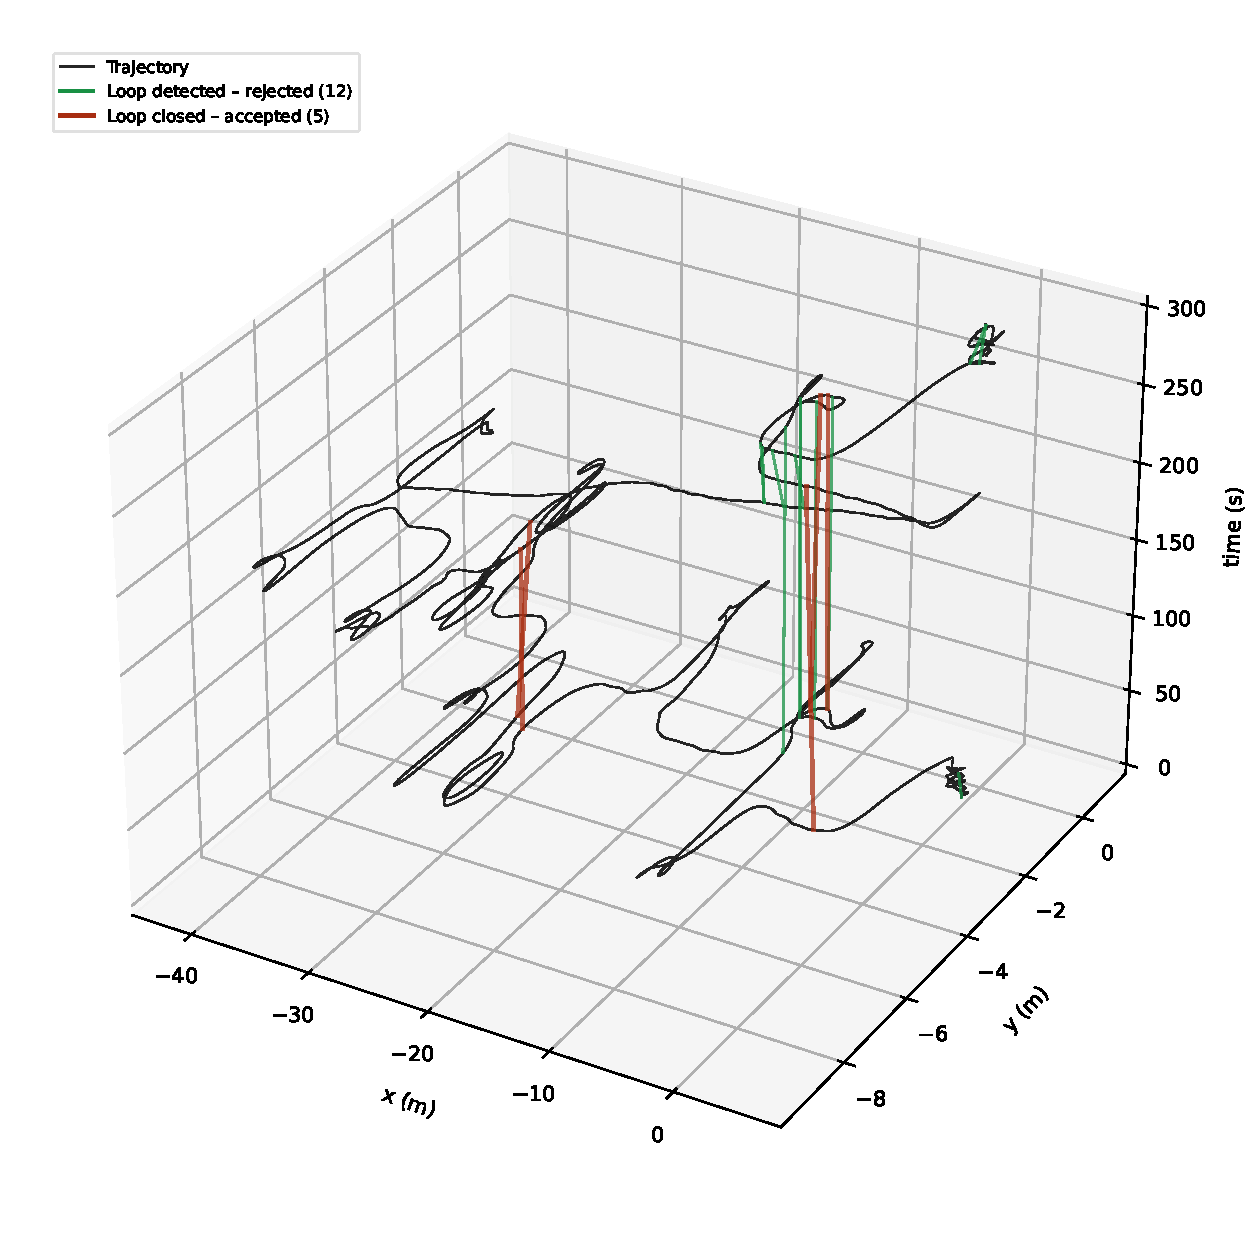
\includegraphics[width=\textwidth]{img/experiments/TC1.loops.pdf}
        \caption{TUM-VI Corridor 1}
        \label{fig:loops_tc1}
    \end{subfigure}
    \hfill
    \begin{subfigure}[b]{0.48\textwidth}
        \centering
        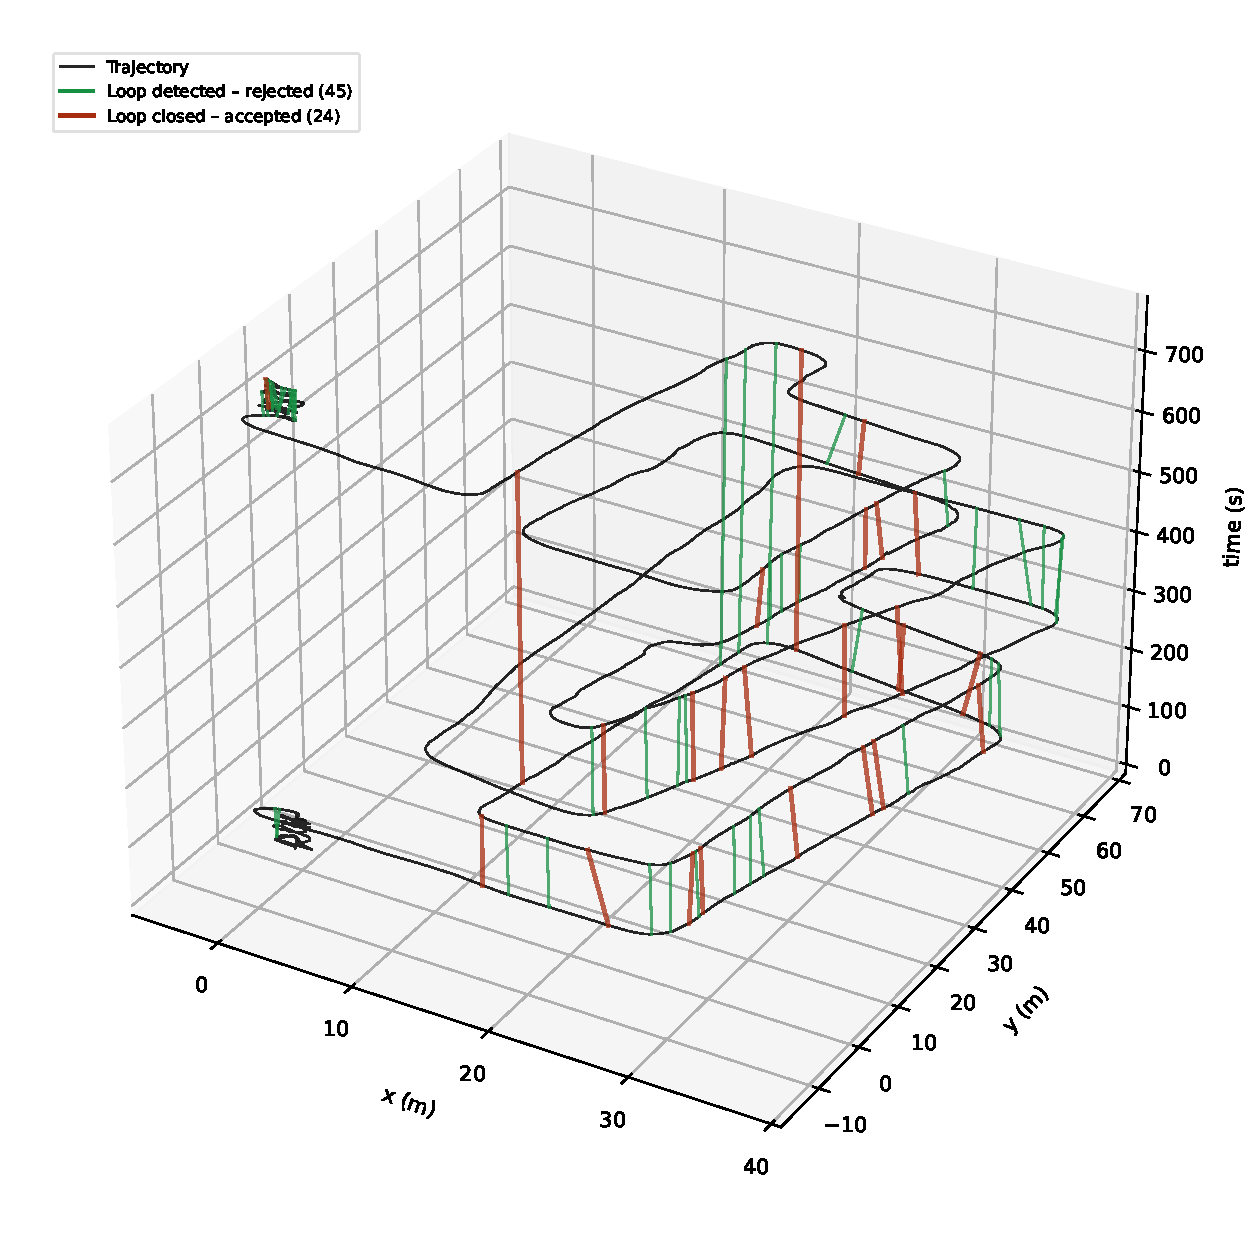
\includegraphics[width=\textwidth]{img/experiments/TM1.loops.pdf}
        \caption{TUM-VI Magistrale 1}
        \label{fig:loops_tm1}
    \end{subfigure}

    \vspace{0.5em}

    \begin{subfigure}[b]{0.48\textwidth}
        \centering
        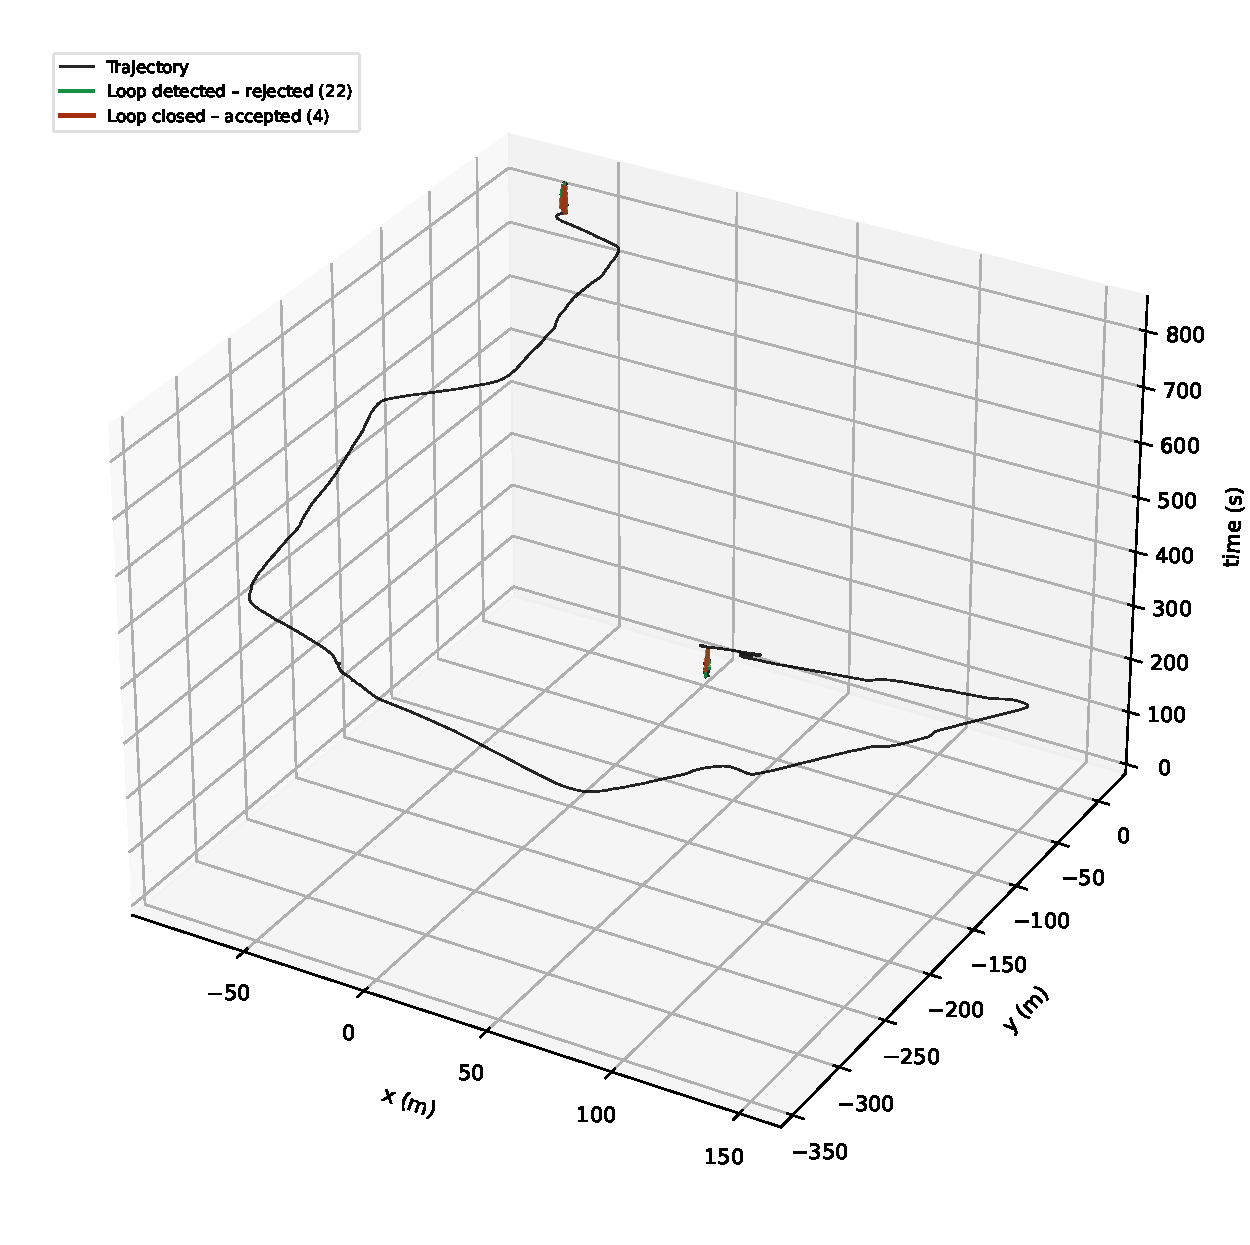
\includegraphics[width=\textwidth]{img/experiments/TO3.loops.pdf}
        \caption{TUM-VI Outdoors 3}
        \label{fig:loops_to3}
    \end{subfigure}
    \hfill
    \begin{subfigure}[b]{0.48\textwidth}
        \centering
        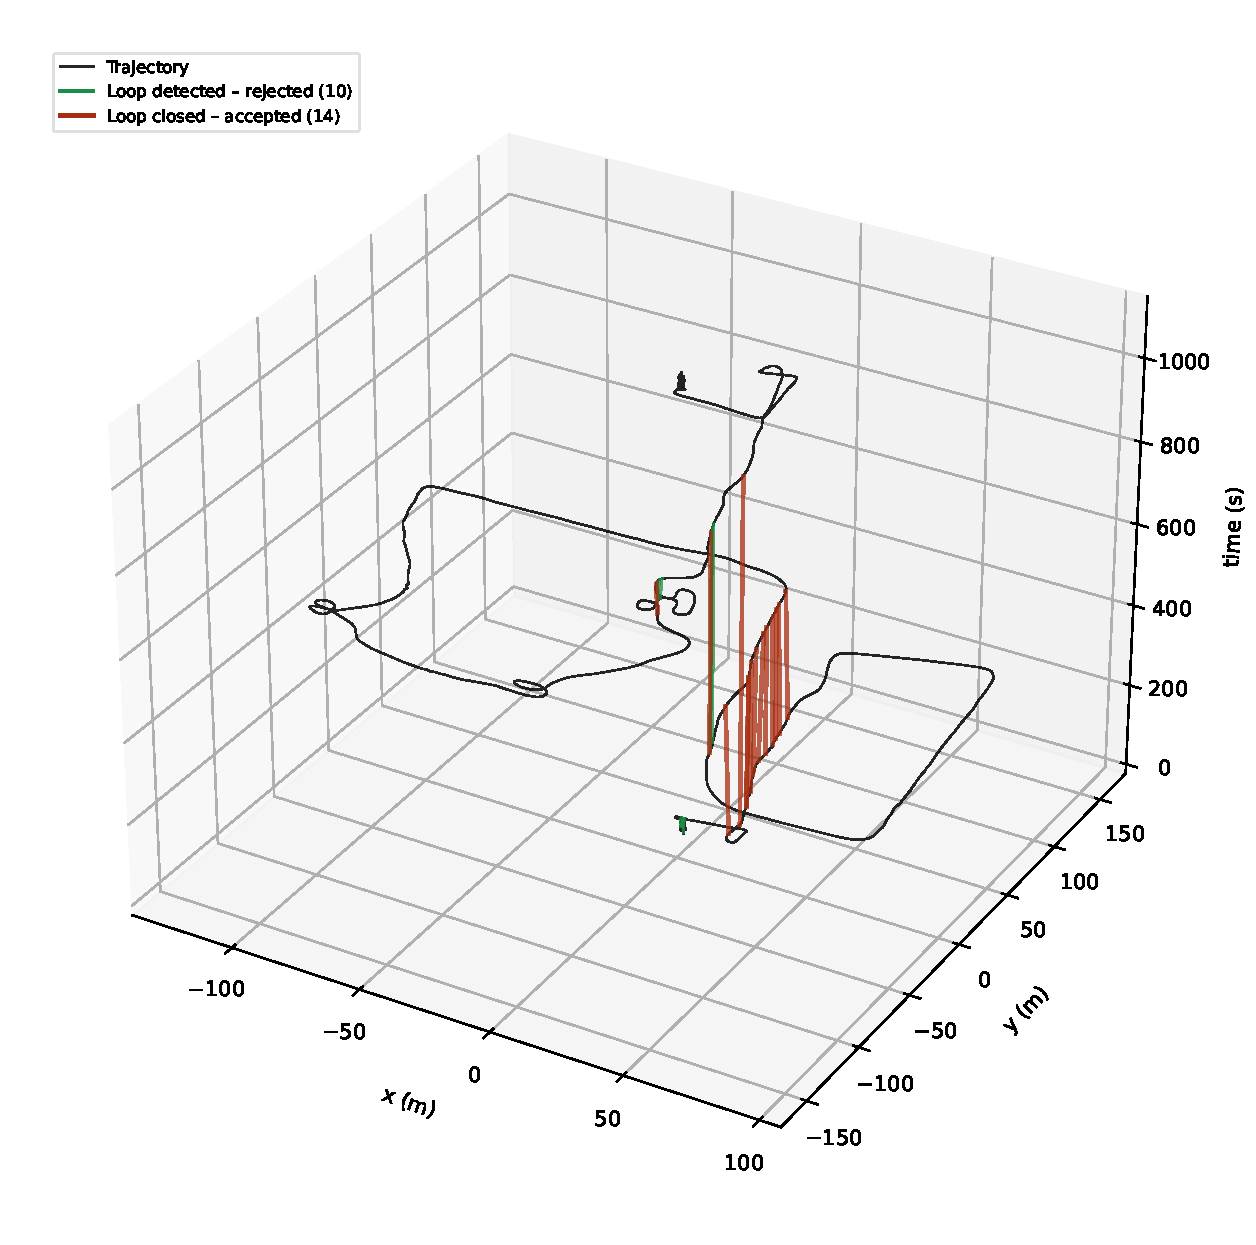
\includegraphics[width=\textwidth]{img/experiments/TO7.loops.pdf}
        \caption{TUM-VI Outdoors 7}
        \label{fig:loops_to7}
    \end{subfigure}

    \caption{Detecciones de ciclo para algunas secuencias del TUM-VI benchmark dataset}
    \label{fig:loops_tumvi}
\end{figure}

En la Tabla \ref{tab:MH_ablation_all} se muestran los resultados de ATE, RTE y ciclos detectados en las secuencias de ``Machine Hall''.
En este caso, el sistema que mayor precisión logra es BasaltLC, aunque la mejora respecto a Basalt original no es tan significativa.
Es interesante que la introducción de RootBA en BasaltSLAM empeora la precisión por unos centímetros. En términos de RTE, todos los sistemas mantienen una precisión similar.

\begin{table}[ht]
\centering
\caption{ATE [cm], RTE [cm] y ciclos detectados en EuRoC Machine Hall.}
\label{tab:MH_ablation_all}
\begin{tabular}{l rrrr | rrrr | rrrr}
\toprule
& \multicolumn{4}{c|}{\textbf{ATE [cm]}} & \multicolumn{4}{c|}{\textbf{RTE [cm]}} & \multicolumn{4}{c}{\textbf{Ciclos}} \\
\cmidrule(lr){2-5} \cmidrule(lr){6-9} \cmidrule(lr){10-13}
\textbf{Secuencia}
& \rotatebox{90}{\textbf{Basalt}\,}
& \rotatebox{90}{\textbf{BasaltLC}\,}
& \rotatebox{90}{\textbf{BasaltSLAM}\,}
& \rotatebox{90}{\textbf{BasaltSLAM-CQ}\,}
& \rotatebox{90}{\textbf{Basalt}\,}
& \rotatebox{90}{\textbf{BasaltLC}\,}
& \rotatebox{90}{\textbf{BasaltSLAM}\,}
& \rotatebox{90}{\textbf{BasaltSLAM-CQ}\,}
& \rotatebox{90}{\textbf{Basalt}\,}
& \rotatebox{90}{\textbf{BasaltLC}\,}
& \rotatebox{90}{\textbf{BasaltSLAM}\,}
& \rotatebox{90}{\textbf{BasaltSLAM-CQ}\,} \\
\midrule
EMH01 & 7.6 & \textbf{6.3} & 8.0 & 8.0 & \textbf{0.5} & \textbf{0.5} & \textbf{0.5} & \textbf{0.5} & -- & 11 & 11 & 10 \\
EMH02 & 4.9 & \textbf{4.8} & 4.9 & 6.4 & \textbf{0.4} & 0.5 & \textbf{0.4} & 0.5 & -- & 11 & 11 & 13 \\
EMH03 & 6.0 & 5.8 & 5.4 & \textbf{4.4} & \textbf{1.2} & \textbf{1.2} & \textbf{1.2} & 1.3 & -- & 24 & 24 & 26 \\
EMH04 & 12.7 & \textbf{9.1} & 13.4 & 13.2 & \textbf{1.3} & \textbf{1.3} & 1.4 & 1.4 & -- & 10 & 10 & 7 \\
EMH05 & 14.5 & \textbf{8.2} & 9.4 & 10.2 & \textbf{1.1} & \textbf{1.1} & \textbf{1.1} & 1.2 & -- & 9 & 9 & 8 \\
\midrule
Mediana & 7.6 & \textbf{6.3} & 8.0 & 8.0 & \textbf{1.1} & \textbf{1.1} & \textbf{1.1} & 1.2 & -- & -- & -- & -- \\
Promedio & 9.1 & \textbf{6.8} & 8.2 & 8.4 & \textbf{0.9} & \textbf{0.9} & \textbf{0.9} & 1.0 & -- & -- & -- & -- \\
\bottomrule
\end{tabular}
\end{table}

En la Tabla \ref{tab:V1_ablation_all} se muestran los resultados de ATE, RTE y ciclos detectados en las secuencias de ``Vicon Room 1''.
En este caso, BasaltSLAM logra una mejora con respecto a Basalt. Sin embargo, para la secuencia EV103, sucede algo similar
a ``Machine Hall'', ya que la introducción de RootBA empeora la precisión.

\begin{table}[ht]
\centering
\caption{ATE [cm], RTE [cm] y ciclos detectados en EuRoC Vicon Room 1.}
\label{tab:V1_ablation_all}
\begin{tabular}{l rrrr | rrrr | rrrr}
\toprule
& \multicolumn{4}{c|}{\textbf{ATE [cm]}} & \multicolumn{4}{c|}{\textbf{RTE [cm]}} & \multicolumn{4}{c}{\textbf{Ciclos}} \\
\cmidrule(lr){2-5} \cmidrule(lr){6-9} \cmidrule(lr){10-13}
\textbf{Secuencia}
& \rotatebox{90}{\textbf{Basalt}\,}
& \rotatebox{90}{\textbf{BasaltLC}\,}
& \rotatebox{90}{\textbf{BasaltSLAM}\,}
& \rotatebox{90}{\textbf{BasaltSLAM-CQ}\,}
& \rotatebox{90}{\textbf{Basalt}\,}
& \rotatebox{90}{\textbf{BasaltLC}\,}
& \rotatebox{90}{\textbf{BasaltSLAM}\,}
& \rotatebox{90}{\textbf{BasaltSLAM-CQ}\,}
& \rotatebox{90}{\textbf{Basalt}\,}
& \rotatebox{90}{\textbf{BasaltLC}\,}
& \rotatebox{90}{\textbf{BasaltSLAM}\,}
& \rotatebox{90}{\textbf{BasaltSLAM-CQ}\,} \\
\midrule
EV101 & 4.4 & 4.5 & \textbf{4.2} & \textbf{4.2} & \textbf{1.3} & \textbf{1.3} & \textbf{1.3} & \textbf{1.3} & -- & 23 & 23 & 16 \\
EV102 & 5.4 & 3.9 & \textbf{2.9} & 4.5 & \textbf{1.1} & 1.2 & 1.2 & 1.2 & -- & 20 & 20 & 18 \\
EV103 & 5.6 & 6.6 & 13.0 & \textbf{5.2} & \textbf{1.2} & 1.4 & 4.1 & 2.1 & -- & 7 & 7 & 7 \\
\midrule
Mediana & 5.4 & 4.5 & \textbf{4.2} & 4.5 & \textbf{1.2} & 1.3 & 1.3 & 1.3 & -- & -- & -- & -- \\
Promedio & 5.1 & 5.0 & 6.7 & \textbf{4.6} & \textbf{1.2} & 1.3 & 2.2 & 1.6 & -- & -- & -- & -- \\
\bottomrule
\end{tabular}
\end{table}

Finalmente, en la Tabla \ref{tab:V2_ablation_all} se muestran los resultados de ATE, RTE y ciclos detectados en las secuencias de ``Vicon Room 2''.
En este caso, BasaltLC es el que logra una mayor precisión en ATE. Aunque en RTE Basalt mantiene el mejor resultado.
Con la introducción de RootBA en BasaltSLAM, se observa una vez más que se reduce la precisión notablemente.

\begin{table}[ht]
\centering
\caption{ATE [cm], RTE [cm] y ciclos detectados en EuRoC Vicon Room 2.}
\label{tab:V2_ablation_all}
\begin{tabular}{l rrrr | rrrr | rrrr}
\toprule
& \multicolumn{4}{c|}{\textbf{ATE [cm]}} & \multicolumn{4}{c|}{\textbf{RTE [cm]}} & \multicolumn{4}{c}{\textbf{Ciclos}} \\
\cmidrule(lr){2-5} \cmidrule(lr){6-9} \cmidrule(lr){10-13}
\textbf{Secuencia}
& \rotatebox{90}{\textbf{Basalt}\,}
& \rotatebox{90}{\textbf{BasaltLC}\,}
& \rotatebox{90}{\textbf{BasaltSLAM}\,}
& \rotatebox{90}{\textbf{BasaltSLAM-CQ}\,}
& \rotatebox{90}{\textbf{Basalt}\,}
& \rotatebox{90}{\textbf{BasaltLC}\,}
& \rotatebox{90}{\textbf{BasaltSLAM}\,}
& \rotatebox{90}{\textbf{BasaltSLAM-CQ}\,}
& \rotatebox{90}{\textbf{Basalt}\,}
& \rotatebox{90}{\textbf{BasaltLC}\,}
& \rotatebox{90}{\textbf{BasaltSLAM}\,}
& \rotatebox{90}{\textbf{BasaltSLAM-CQ}\,} \\
\midrule
EV201 & \textbf{3.6} & \textbf{3.6} & 3.8 & 3.7 & \textbf{0.3} & 0.4 & \textbf{0.3} & 0.5 & -- & 2 & 2 & 2 \\
EV202 & 4.0 & \textbf{3.8} & 9.5 & 6.6 & \textbf{0.7} & 0.9 & 5.3 & 4.2 & -- & 16 & 16 & 18 \\
EV203 & 15.6 & \textbf{7.6} & 13.9 & 21.3 & \textbf{2.6} & 3.3 & 6.0 & 8.8 & -- & 7 & 7 & 4 \\
\midrule
Mediana & 4.0 & \textbf{3.8} & 9.5 & 6.6 & \textbf{0.7} & 0.9 & 5.3 & 4.2 & -- & -- & -- & -- \\
Promedio & 7.8 & \textbf{5.0} & 9.1 & 10.6 & \textbf{1.2} & 1.5 & 3.9 & 4.5 & -- & -- & -- & -- \\
\bottomrule
\end{tabular}
\end{table}


\begin{figure}[ht]
    \centering
    \begin{subfigure}[b]{0.48\textwidth}
        \centering
        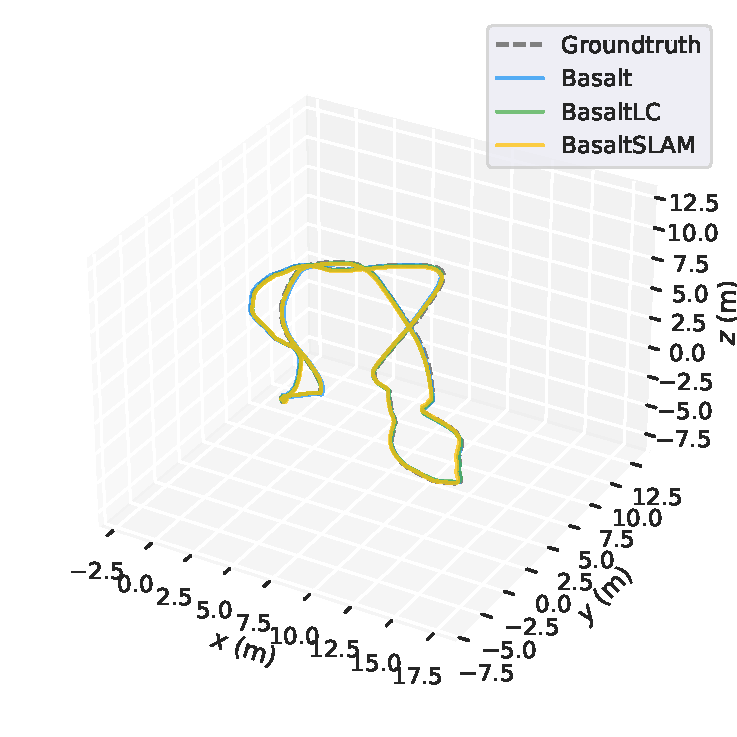
\includegraphics[width=\textwidth]{img/experiments/MH_04.traj.pdf}
        \caption{Machine Hall - Secuencia 4}
        \label{fig:traj_mh04}
    \end{subfigure}
    \hfill
    \begin{subfigure}[b]{0.48\textwidth}
        \centering
        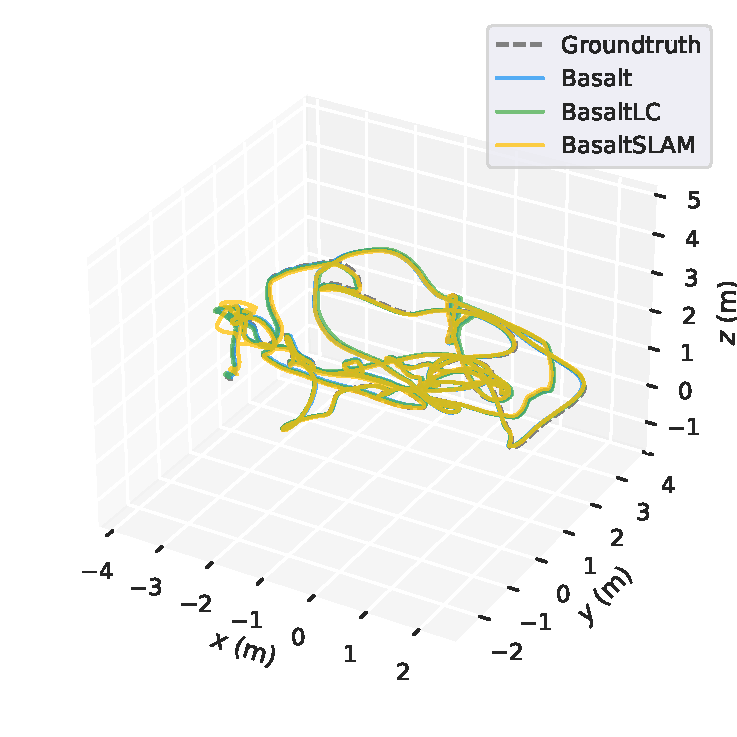
\includegraphics[width=\textwidth]{img/experiments/V2_02.traj.pdf}
        \caption{Vicon Room 2 - Secuencia 2}
        \label{fig:traj_v202}
    \end{subfigure}

    \vspace{0.5em}

    \begin{subfigure}[b]{0.48\textwidth}
        \centering
        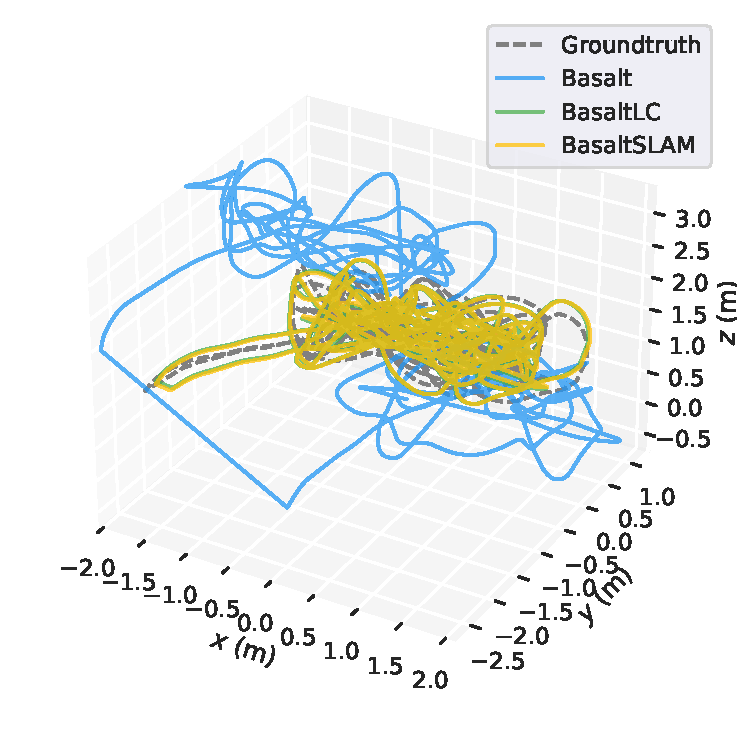
\includegraphics[width=\textwidth]{img/experiments/TM1.traj.pdf}
        \caption{TUM-VI Magistrale 1}
        \label{fig:traj_tm1}
    \end{subfigure}
    \hfill
    \begin{subfigure}[b]{0.48\textwidth}
        \centering
        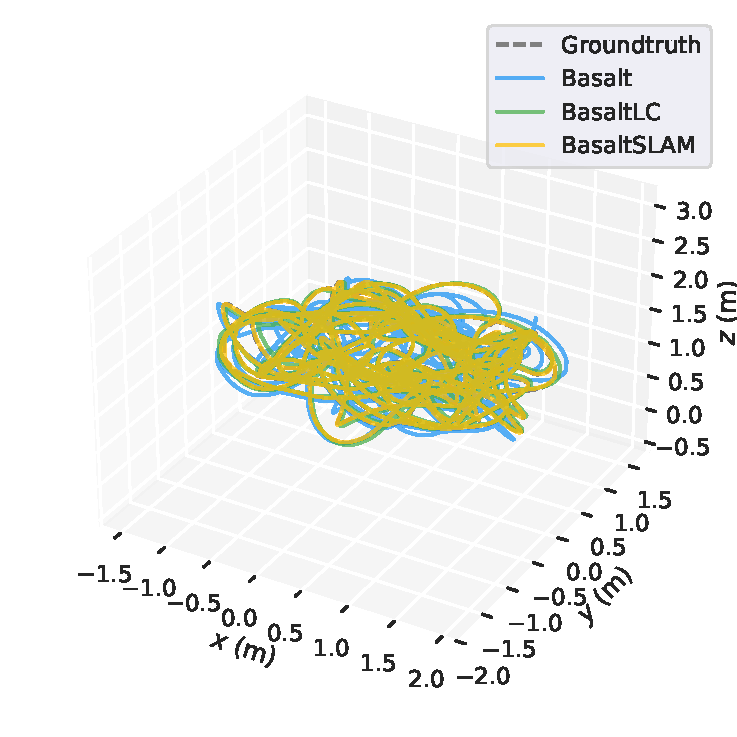
\includegraphics[width=\textwidth]{img/experiments/TR5.traj.pdf}
        \caption{TUM-VI Room 5}
        \label{fig:traj_tr5}
    \end{subfigure}

    \caption{Comparativa de las trayectorias estimadas por Basalt, BasaltLC y BasaltSLAM para algunas secuencias del TUM-VI benchmark dataset y EuRoC MAV dataset.}
    \label{fig:trajectories}
\end{figure}


\subsection{Resultados en datasets de XR} \label{sec:results_xr}

En la Tabla \ref{tab:msdmi_ablation_all} se muestran los resultados de ATE, RTE y ciclos detectados en las secuencias de MI*.
Se observa que, en gran parte de las secuencias, se detecta un gran número de ciclos. Esto hace que BasaltLC logre reducir
la mediana del ATE en más de un 85\%, en comparación con Basalt. Más aún, con la incorporación de RootBA en BasaltSLAM, se consigue
una mejora adicional, logrando una precisión menor a 3 cm en la mayoría de las secuencias.
En cuanto a BasaltSLAM-CQ, en algunas secuencias se observan mejoras destacables, como en MIPB02 o MIO16. Sin embargo,
en la secuencia MIO01, la incorporación de la consulta de covisibilidad provoca que el sistema pierda la localización. Esto puede
atribuirse a la reidentificación incorrecta de un landmark, aunque se trata de un problema que requiere investigación más profunda.
Además, el sistema no logra completar la secuencia MIPB08, de más de 35 minutos de duración. La causa reside en que,
según el diseño actual del sistema, para reidentificar landmarks se almacenan los parches de todos los keypoints
detectados desde el inicio de la secuencia. A medida que esta avanza, el número de parches almacenados crece indefinidamente
hasta agotar la memoria disponible.
En términos de RTE, Basalt es el sistema que logra la mejor precisión, aunque BasaltLC y BasaltSLAM logran una precisión similar.

\begin{table}[ht]
\centering
\caption{ATE [cm], RTE [cm] y ciclos detectados en MSD Valve Index.}
\label{tab:msdmi_ablation_all}
\begin{tabular}{l rrrr | rrrr | rrrr}
\toprule
& \multicolumn{4}{c|}{\textbf{ATE [cm]}} & \multicolumn{4}{c|}{\textbf{RTE [cm]}} & \multicolumn{4}{c}{\textbf{Ciclos}} \\
\cmidrule(lr){2-5} \cmidrule(lr){6-9} \cmidrule(lr){10-13}
\textbf{Secuencia}
& \rotatebox{90}{\textbf{Basalt}\,}
& \rotatebox{90}{\textbf{BasaltLC}\,}
& \rotatebox{90}{\textbf{BasaltSLAM}\,}
& \rotatebox{90}{\textbf{BasaltSLAM-CQ}\,}
& \rotatebox{90}{\textbf{Basalt}\,}
& \rotatebox{90}{\textbf{BasaltLC}\,}
& \rotatebox{90}{\textbf{BasaltSLAM}\,}
& \rotatebox{90}{\textbf{BasaltSLAM-CQ}\,}
& \rotatebox{90}{\textbf{Basalt}\,}
& \rotatebox{90}{\textbf{BasaltLC}\,}
& \rotatebox{90}{\textbf{BasaltSLAM}\,}
& \rotatebox{90}{\textbf{BasaltSLAM-CQ}\,} \\
\midrule
MIO01 & 62.0 & 22.4 & \textbf{18.7} & 3787.2 & \textbf{3.7} & 4.4 & 4.4 & 603.5 & -- & 273 & 273 & 118 \\
MIO02 & 118.3 & 32.0 & \textbf{23.6} & 37.5 & 6.5 & 6.3 & \textbf{4.0} & 6.1 & -- & 91 & 91 & 40 \\
MIO03 & 9.4 & 5.7 & \textbf{2.5} & 3.4 & \textbf{0.6} & 0.7 & 1.0 & 1.2 & -- & 138 & 138 & 62 \\
MIO04 & 20.7 & \textbf{7.0} & 7.4 & 8.0 & \textbf{1.3} & 1.5 & 3.6 & 4.0 & -- & 182 & 182 & 109 \\
MIO05 & 3.4 & 3.8 & 1.9 & \textbf{1.6} & \textbf{0.3} & 0.5 & \textbf{0.3} & 0.4 & -- & 94 & 94 & 38 \\
MIO06 & 4.9 & 4.5 & 2.6 & \textbf{2.4} & \textbf{1.0} & 1.3 & 1.4 & 1.2 & -- & 131 & 131 & 78 \\
MIO07 & 2.3 & 4.2 & \textbf{1.2} & 2.3 & \textbf{0.2} & 0.5 & \textbf{0.2} & 0.5 & -- & 29 & 29 & 13 \\
MIO08 & 5.7 & \textbf{2.9} & 6.9 & 4.3 & \textbf{0.7} & 0.8 & 3.9 & 1.6 & -- & 3 & 3 & 1 \\
MIO09 & 0.6 & 0.6 & \textbf{0.2} & 0.5 & 0.3 & 0.3 & \textbf{0.2} & 0.4 & -- & 0 & 0 & 0 \\
MIO10 & \textbf{1.5} & 1.6 & 1.8 & 2.7 & \textbf{0.5} & \textbf{0.5} & 0.6 & 0.7 & -- & 0 & 0 & 0 \\
MIO11 & 2.4 & 2.5 & \textbf{2.3} & 3.3 & 0.7 & 0.7 & \textbf{0.6} & 1.2 & -- & 0 & 0 & 0 \\
MIO12 & 43.5 & 4.8 & \textbf{4.2} & 4.3 & \textbf{0.6} & \textbf{0.6} & \textbf{0.6} & 0.8 & -- & 221 & 221 & 146 \\
MIO13 & 108.4 & 28.5 & 28.0 & \textbf{25.5} & 2.9 & 2.8 & \textbf{2.7} & 3.1 & -- & 130 & 130 & 72 \\
MIO14 & 9.7 & 3.7 & \textbf{2.5} & 3.4 & \textbf{0.3} & \textbf{0.3} & \textbf{0.3} & 0.4 & -- & 171 & 171 & 68 \\
MIO15 & 79.5 & 12.4 & \textbf{10.7} & 13.5 & \textbf{1.2} & 1.3 & 1.3 & 1.7 & -- & 197 & 197 & 92 \\
MIO16 & 53.1 & 13.3 & 18.7 & \textbf{9.1} & \textbf{1.3} & \textbf{1.3} & 2.5 & 1.7 & -- & 57 & 57 & 41 \\
MIPB01 & 27.9 & 3.5 & \textbf{1.3} & \textbf{1.3} & 0.7 & 1.0 & \textbf{0.6} & \textbf{0.6} & -- & 686 & 686 & 283 \\
MIPB02 & 23.5 & 3.7 & 3.5 & \textbf{1.8} & \textbf{0.5} & 0.9 & 2.7 & \textbf{0.5} & -- & 492 & 492 & 208 \\
MIPB03 & 18.9 & 4.3 & \textbf{2.9} & 3.7 & \textbf{0.6} & 0.7 & 0.7 & 1.3 & -- & 609 & 609 & 284 \\
MIPB04 & 10.4 & 4.3 & 2.0 & \textbf{1.8} & \textbf{0.5} & 0.6 & 0.6 & \textbf{0.5} & -- & 433 & 433 & 151 \\
MIPB05 & 4.4 & 3.2 & \textbf{1.4} & 2.7 & \textbf{0.4} & 0.6 & 0.5 & \textbf{0.4} & -- & 459 & 459 & 147 \\
MIPB06 & 4.8 & 4.0 & 2.9 & \textbf{1.9} & \textbf{0.4} & 0.5 & 0.5 & 0.5 & -- & 310 & 310 & 117 \\
MIPB07 & 6.2 & 3.5 & \textbf{1.6} & 1.8 & \textbf{0.5} & 0.6 & \textbf{0.5} & 0.6 & -- & 490 & 490 & 139 \\
MIPB08 & 63.0 & 4.5 & \textbf{3.9} & -- & \textbf{0.4} & \textbf{0.4} & 0.5 & -- & -- & 1264 & 1264 & -- \\
MIPP01 & 43.9 & 4.5 & 2.9 & \textbf{2.8} & \textbf{1.0} & 1.2 & 1.1 & 1.3 & -- & 632 & 632 & 329 \\
MIPP02 & 24.1 & 4.1 & 3.9 & \textbf{3.1} & \textbf{1.0} & 1.2 & 1.7 & 1.5 & -- & 354 & 354 & 171 \\
MIPP03 & 26.9 & 4.4 & 4.8 & \textbf{3.2} & \textbf{0.9} & 1.0 & 2.3 & 1.4 & -- & 507 & 507 & 271 \\
MIPP04 & 28.7 & 4.0 & 2.5 & \textbf{2.4} & \textbf{0.8} & 0.9 & 1.0 & 1.0 & -- & 544 & 544 & 300 \\
MIPP05 & 18.3 & 3.1 & \textbf{2.7} & \textbf{2.7} & \textbf{0.6} & 0.7 & 1.9 & 1.2 & -- & 407 & 407 & 223 \\
MIPP06 & 28.3 & 3.9 & 2.7 & \textbf{2.3} & \textbf{1.0} & 1.1 & 1.2 & \textbf{1.0} & -- & 806 & 806 & 434 \\
MIPT01 & 10.6 & 4.3 & \textbf{1.7} & 1.9 & \textbf{0.4} & 0.6 & 0.5 & 0.6 & -- & 723 & 723 & 333 \\
MIPT02 & 19.8 & 3.5 & \textbf{2.1} & \textbf{2.1} & \textbf{0.4} & 0.5 & 0.5 & 0.5 & -- & 1189 & 1189 & 616 \\
MIPT03 & 39.9 & 4.0 & \textbf{3.5} & \textbf{3.5} & \textbf{0.6} & 0.7 & \textbf{0.6} & 0.7 & -- & 1178 & 1178 & 517 \\
\midrule
Mediana & 19.8 & 4.1 & \textbf{2.7} & 2.8 & \textbf{0.6} & 0.7 & 0.7 & 1.0 & -- & -- & -- & -- \\
Promedio & 28.0 & 6.6 & \textbf{5.4} & 123.4 & \textbf{1.0} & 1.1 & 1.4 & 20.1 & -- & -- & -- & -- \\
\bottomrule
\end{tabular}
\end{table}

En la Tabla \ref{tab:msdmg_ablation_all} se muestran los resultados de ATE, RTE y ciclos detectados en las secuencias de MG*.
Se observan resultados similares a los obtenidos en las secuencias de MI*. BasaltSLAM es el sistema que logra la mejor precisión,
mejorando la mediana del ATE en más de un 70\% en comparación con Basalt. La incorporación de la consulta de covisibilidad en BasaltSLAM-CQ
consigue un resultado destacado en la secuencia MGO01. No obstante, el problema de memoria previamente descrito impide que
el sistema complete la secuencia MGO12, de más de 40 minutos de duración.
En términos de RTE, BasaltSLAM consigue mayor precisión en la mayoría de secuencias, aunque todos mantienen una precisión similar.

\begin{table}[ht]
\centering
\caption{ATE [cm], RTE [cm] y ciclos detectados en MSD HP Reverb G2.}
\label{tab:msdmg_ablation_all}
\begin{tabular}{l rrrr | rrrr | rrrr}
\toprule
& \multicolumn{4}{c|}{\textbf{ATE [cm]}} & \multicolumn{4}{c|}{\textbf{RTE [cm]}} & \multicolumn{4}{c}{\textbf{Ciclos}} \\
\cmidrule(lr){2-5} \cmidrule(lr){6-9} \cmidrule(lr){10-13}
\textbf{Secuencia}
& \rotatebox{90}{\textbf{Basalt}\,}
& \rotatebox{90}{\textbf{BasaltLC}\,}
& \rotatebox{90}{\textbf{BasaltSLAM}\,}
& \rotatebox{90}{\textbf{BasaltSLAM-CQ}\,}
& \rotatebox{90}{\textbf{Basalt}\,}
& \rotatebox{90}{\textbf{BasaltLC}\,}
& \rotatebox{90}{\textbf{BasaltSLAM}\,}
& \rotatebox{90}{\textbf{BasaltSLAM-CQ}\,}
& \rotatebox{90}{\textbf{Basalt}\,}
& \rotatebox{90}{\textbf{BasaltLC}\,}
& \rotatebox{90}{\textbf{BasaltSLAM}\,}
& \rotatebox{90}{\textbf{BasaltSLAM-CQ}\,} \\
\midrule
MGO01 & 68.0 & 13.4 & 12.1 & \textbf{3.4} & \textbf{2.3} & 2.5 & 2.4 & 2.7 & -- & 43 & 43 & 40 \\
MGO02 & 55.6 & 8.3 & 7.5 & \textbf{6.2} & \textbf{2.8} & 3.0 & 3.1 & 5.6 & -- & 82 & 82 & 76 \\
MGO03 & 14.5 & 4.2 & \textbf{1.7} & \textbf{1.7} & 1.3 & 1.5 & \textbf{1.1} & 1.2 & -- & 122 & 122 & 98 \\
MGO04 & 26.1 & 6.7 & \textbf{5.4} & 5.7 & \textbf{2.5} & 2.7 & 2.8 & 3.7 & -- & 62 & 62 & 51 \\
MGO05 & 3.0 & 3.0 & \textbf{1.7} & \textbf{1.7} & 0.4 & 0.5 & \textbf{0.3} & 0.4 & -- & 81 & 81 & 65 \\
MGO06 & 11.1 & 5.2 & 4.1 & \textbf{3.1} & 1.8 & 2.0 & \textbf{1.6} & 1.9 & -- & 94 & 94 & 78 \\
MGO07 & 2.1 & 2.1 & \textbf{1.4} & 1.5 & 0.6 & 0.6 & \textbf{0.4} & 0.5 & -- & 23 & 23 & 14 \\
MGO08 & \textbf{2.7} & 2.8 & 5.0 & 3.8 & \textbf{1.3} & 1.4 & 3.5 & 2.4 & -- & 2 & 2 & 0 \\
MGO09 & \textbf{0.8} & \textbf{0.8} & 1.1 & 1.0 & \textbf{0.6} & 0.7 & 0.7 & 0.7 & -- & 0 & 0 & 0 \\
MGO10 & \textbf{0.8} & 0.9 & 1.4 & 1.2 & 0.4 & 0.4 & \textbf{0.3} & \textbf{0.3} & -- & 0 & 0 & 0 \\
MGO11 & 1.7 & 1.7 & \textbf{1.0} & \textbf{1.0} & 0.6 & 0.6 & \textbf{0.4} & 0.5 & -- & 0 & 0 & 0 \\
MGO12 & 60.7 & 5.8 & \textbf{5.4} & -- & \textbf{1.7} & 1.8 & \textbf{1.7} & -- & -- & 931 & 931 & -- \\
MGO13 & 68.4 & 8.6 & 8.6 & \textbf{8.2} & \textbf{2.6} & 2.7 & 4.1 & 6.1 & -- & 43 & 43 & 34 \\
MGO14 & 7.0 & 3.9 & \textbf{1.9} & 2.2 & 1.2 & 1.4 & \textbf{0.9} & 1.1 & -- & 82 & 82 & 70 \\
MGO15 & 3.5 & 4.1 & 1.9 & \textbf{1.3} & 0.4 & 0.4 & \textbf{0.3} & \textbf{0.3} & -- & 30 & 30 & 28 \\
\midrule
Mediana & 7.0 & 4.1 & \textbf{1.9} & 2.0 & 1.3 & 1.4 & \textbf{1.1} & 1.2 & -- & -- & -- & -- \\
Promedio & 21.7 & 4.8 & 4.0 & \textbf{3.0} & \textbf{1.4} & 1.5 & 1.6 & 2.0 & -- & -- & -- & -- \\
\bottomrule
\end{tabular}
\end{table}

En la Tabla \ref{tab:msdmo_ablation_all} se muestran los resultados de ATE, RTE y ciclos detectados en las secuencias de MO*.
Una vez más, BasaltSLAM es el que consigue los mejores resultados en ATE, mejorando la mediana en un 50\% en comparación con Basalt.
La incorporación de la consulta de covisibilidad en BasaltSLAM-CQ logra la mayor precisión en algunas secuencias, con un
resultado especialmente destacado en MOO15, donde es el único sistema que mantiene la localización. Además,
se repite el problema de memoria previamente descrito, que impide al sistema completar la secuencia MOO12,
de más de 40 minutos de duración.
En términos de RTE, Basalt obtiene la mejor mediana y promedio, aunque todos los sistemas mantienen una precisión similar.

\begin{table}[ht]
\centering
\caption{ATE [cm], RTE [cm] y ciclos detectados en MSD Samsung Odyssey+.}
\label{tab:msdmo_ablation_all}
\begin{tabular}{l rrrr | rrrr | rrrr}
\toprule
& \multicolumn{4}{c|}{\textbf{ATE [cm]}} & \multicolumn{4}{c|}{\textbf{RTE [cm]}} & \multicolumn{4}{c}{\textbf{Ciclos}} \\
\cmidrule(lr){2-5} \cmidrule(lr){6-9} \cmidrule(lr){10-13}
\textbf{Secuencia}
& \rotatebox{90}{\textbf{Basalt}\,}
& \rotatebox{90}{\textbf{BasaltLC}\,}
& \rotatebox{90}{\textbf{BasaltSLAM}\,}
& \rotatebox{90}{\textbf{BasaltSLAM-CQ}\,}
& \rotatebox{90}{\textbf{Basalt}\,}
& \rotatebox{90}{\textbf{BasaltLC}\,}
& \rotatebox{90}{\textbf{BasaltSLAM}\,}
& \rotatebox{90}{\textbf{BasaltSLAM-CQ}\,}
& \rotatebox{90}{\textbf{Basalt}\,}
& \rotatebox{90}{\textbf{BasaltLC}\,}
& \rotatebox{90}{\textbf{BasaltSLAM}\,}
& \rotatebox{90}{\textbf{BasaltSLAM-CQ}\,} \\
\midrule
MOO01 & 28.1 & 4.4 & \textbf{3.4} & 4.7 & \textbf{1.7} & 1.8 & \textbf{1.7} & 1.9 & -- & 113 & 113 & 86 \\
MOO02 & 23.8 & 4.2 & 5.0 & \textbf{3.7} & \textbf{1.5} & 1.6 & 3.1 & 1.9 & -- & 129 & 129 & 111 \\
MOO03 & 17.7 & 4.7 & 3.7 & \textbf{3.2} & 1.4 & 1.5 & \textbf{1.2} & 1.8 & -- & 68 & 68 & 51 \\
MOO04 & 6.5 & \textbf{3.8} & 4.2 & 6.3 & \textbf{1.0} & 1.1 & 1.6 & 2.3 & -- & 65 & 65 & 52 \\
MOO05 & 1.8 & 1.9 & 1.2 & \textbf{1.0} & \textbf{0.3} & \textbf{0.3} & \textbf{0.3} & \textbf{0.3} & -- & 16 & 16 & 13 \\
MOO06 & 5.6 & 4.3 & 2.5 & \textbf{1.4} & \textbf{0.8} & 0.9 & 1.0 & \textbf{0.8} & -- & 68 & 68 & 62 \\
MOO07 & 1.3 & 1.3 & 1.3 & \textbf{1.2} & \textbf{0.3} & 0.4 & \textbf{0.3} & \textbf{0.3} & -- & 3 & 3 & 2 \\
MOO08 & \textbf{2.8} & 2.9 & 3.0 & 6.9 & \textbf{1.1} & 1.4 & 1.2 & 2.6 & -- & 0 & 0 & 0 \\
MOO09 & \textbf{0.4} & \textbf{0.4} & 0.5 & 0.5 & \textbf{0.3} & \textbf{0.3} & \textbf{0.3} & \textbf{0.3} & -- & 0 & 0 & 0 \\
MOO10 & \textbf{1.0} & \textbf{1.0} & 1.4 & 1.5 & \textbf{0.4} & \textbf{0.4} & \textbf{0.4} & 0.5 & -- & 0 & 0 & 0 \\
MOO11 & 1.9 & 1.9 & 1.9 & \textbf{1.6} & \textbf{0.5} & \textbf{0.5} & \textbf{0.5} & 0.6 & -- & 0 & 0 & 0 \\
MOO12 & 69.0 & \textbf{8.5} & 10.6 & -- & \textbf{0.8} & \textbf{0.8} & 1.0 & -- & -- & 525 & 525 & -- \\
MOO13 & 50.1 & 7.7 & 7.7 & \textbf{6.6} & \textbf{1.7} & \textbf{1.7} & 2.9 & 3.4 & -- & 71 & 71 & 59 \\
MOO14 & 11.3 & 4.9 & \textbf{3.0} & 4.6 & \textbf{0.8} & 0.9 & 1.7 & 1.7 & -- & 77 & 77 & 68 \\
MOO15 & 205.3 & 292.3 & 291.1 & \textbf{6.6} & 4.3 & 6.3 & 11.0 & \textbf{1.0} & -- & 7 & 7 & 2 \\
MOO16 & 1.4 & 1.4 & 1.2 & \textbf{0.4} & 0.2 & 0.2 & \textbf{0.1} & \textbf{0.1} & -- & 0 & 0 & 0 \\
\midrule
Mediana & 6.1 & 4.0 & \textbf{3.0} & 3.2 & \textbf{0.8} & 0.9 & 1.1 & 1.0 & -- & -- & -- & -- \\
Promedio & 26.7 & 21.6 & 21.3 & \textbf{3.4} & \textbf{1.1} & 1.3 & 1.8 & 1.3 & -- & -- & -- & -- \\
\bottomrule
\end{tabular}
\end{table}

En la Figura \ref{fig:msd_ablation_trajectories} se muestran algunas trayectorias estimadas por los diferentes sistemas en las secuencias de MSD.
Se puede observar, de manera cualitativa, el impacto de las detecciones y cierres de ciclos en las trayectorias estimadas.

Además, en las Figuras \ref{fig:mipp01_ablation_maps} y \ref{fig:mgo01_ablation_maps} se muestran los mapas obtenidos por los diferentes sistemas en las secuencias
MIPP01 y MGO01 respectivamente. Se puede observar la reducción de outliers al incorporar cierres de ciclo y culling de keyframes en BasaltLC.
En BasaltSLAM se puede observar una mejora en la densidad de puntos, con un mapa más detallado, debido a la optimización global
de RootBA.

\begin{figure}[ht]
    \centering
    \begin{subfigure}[b]{0.48\textwidth}
        \centering
        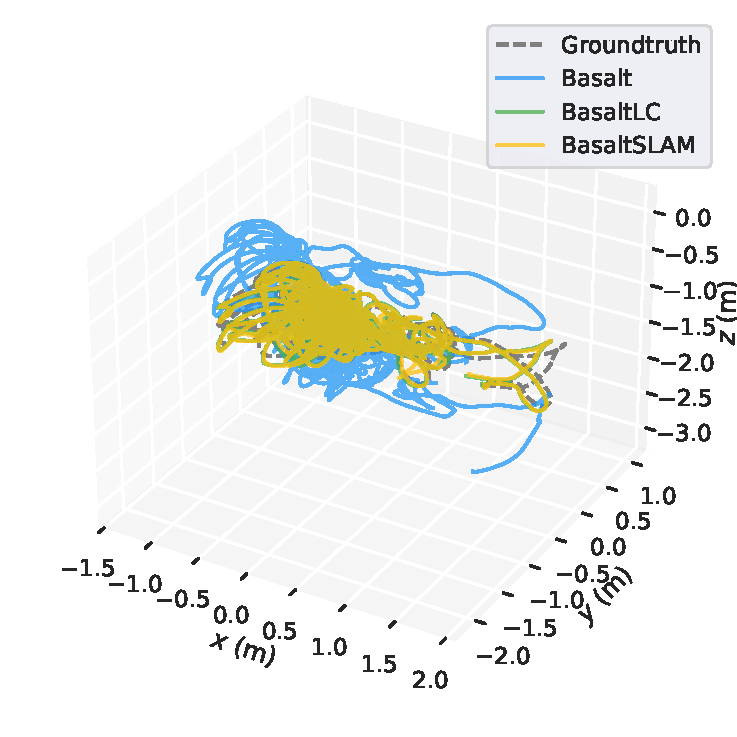
\includegraphics[width=\textwidth]{img/experiments/MOO13.traj.pdf}
        \caption{MOO13}
        \label{fig:traj_moo13}
    \end{subfigure}
    \hfill
    \begin{subfigure}[b]{0.48\textwidth}
        \centering
        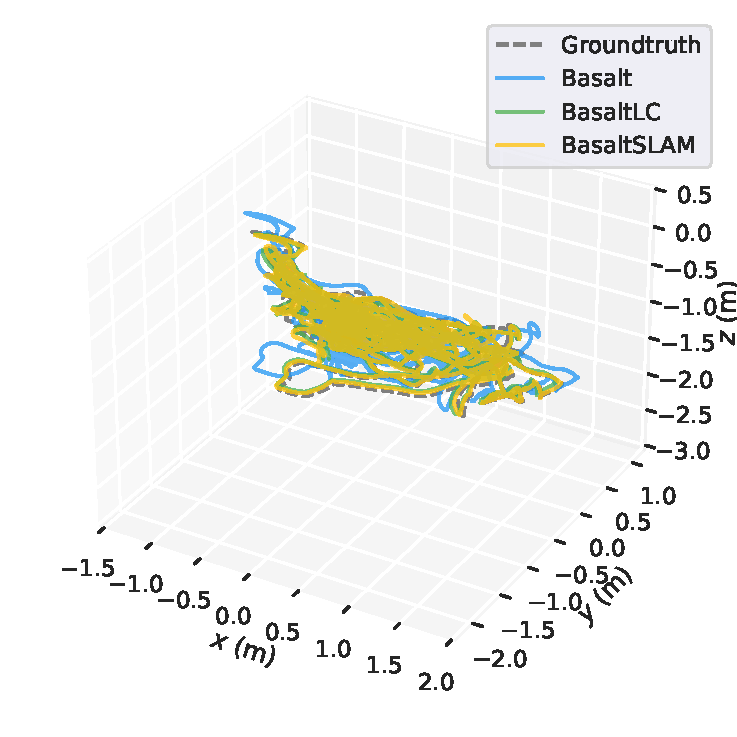
\includegraphics[width=\textwidth]{img/experiments/MGO04.traj.pdf}
        \caption{MGO04}
        \label{fig:traj_mgo04}
    \end{subfigure}

    \vspace{0.5em}

    \begin{subfigure}[b]{0.48\textwidth}
        \centering
        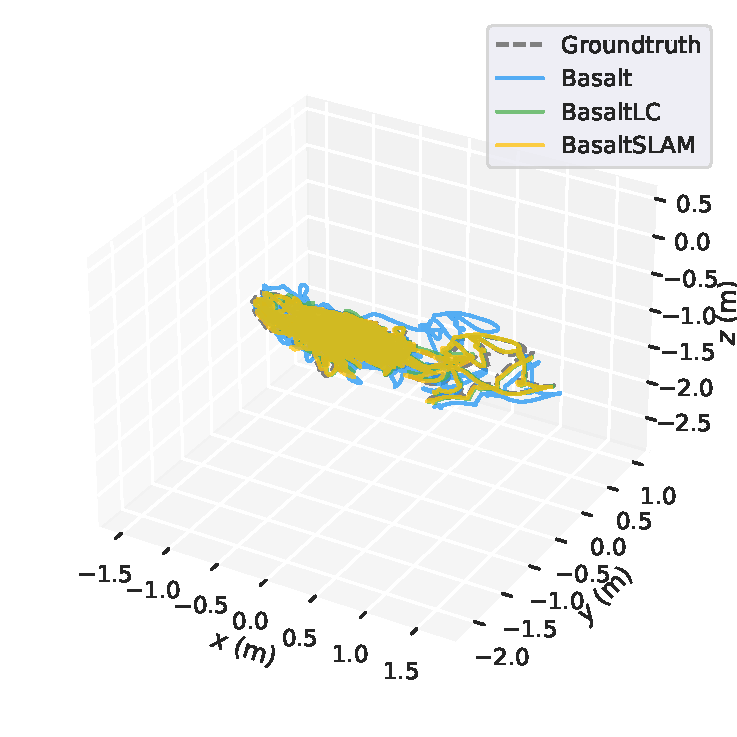
\includegraphics[width=\textwidth]{img/experiments/MIPT02.traj.pdf}
        \caption{MIPT02}
        \label{fig:traj_mipt02}
    \end{subfigure}
    \hfill
    \begin{subfigure}[b]{0.48\textwidth}
        \centering
        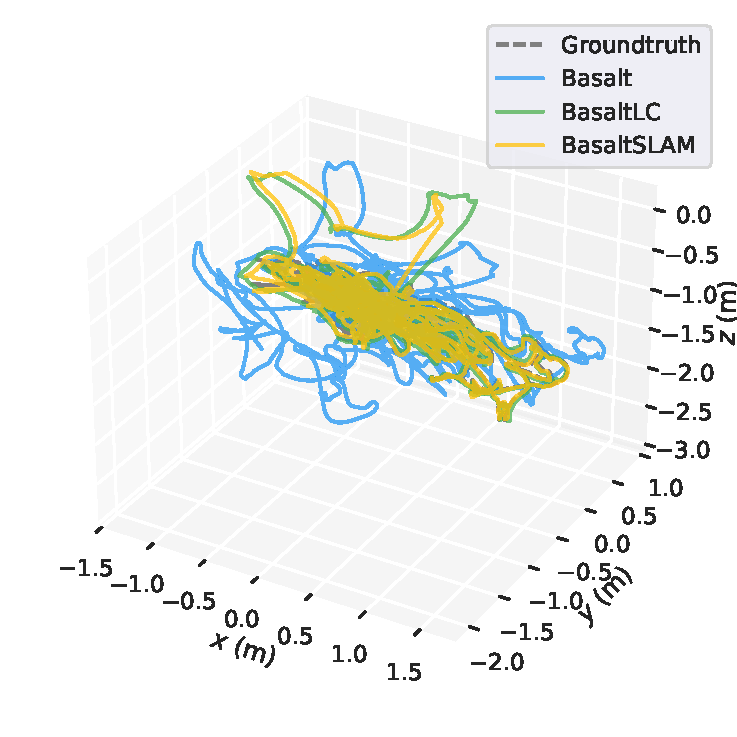
\includegraphics[width=\textwidth]{img/experiments/MIO01.traj.pdf}
        \caption{MIO01}
        \label{fig:traj_mio01}
    \end{subfigure}

    \caption{Comparativa de las trayectorias estimadas por Basalt, BasaltLC y BasaltSLAM para algunas secuencias de MSD.}
    \label{fig:msd_ablation_trajectories}
\end{figure}

\begin{figure}[ht]
    \centering
    \begin{subfigure}[b]{0.32\textwidth}
        \centering
        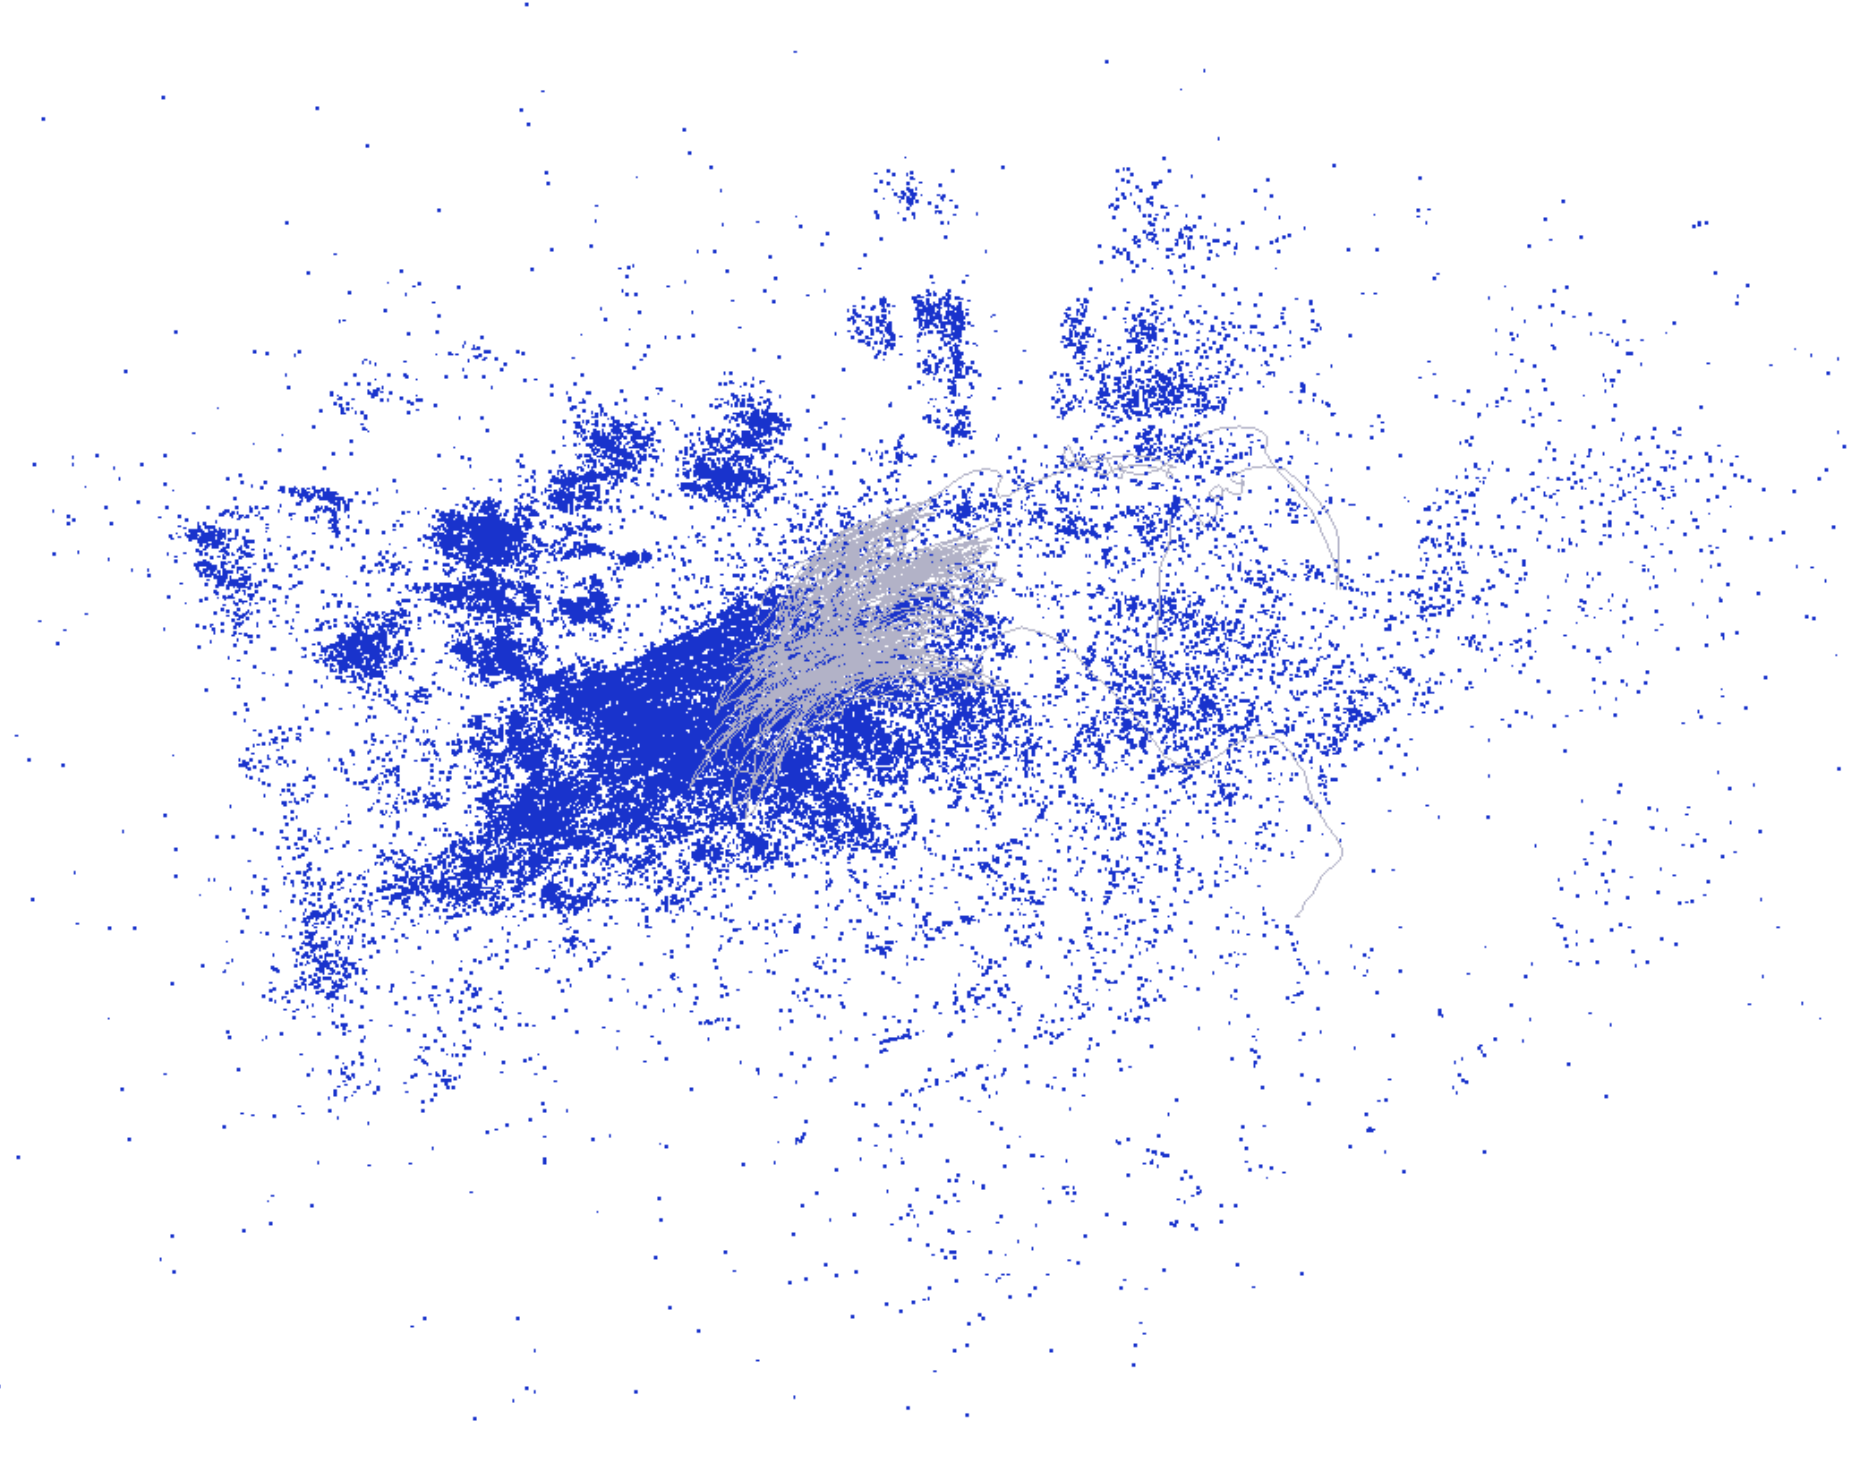
\includegraphics[width=\textwidth]{img/experiments/MIPP01.vio.map.png}
        \caption{Basalt}
        \label{fig:mipp01_basalt_map}
    \end{subfigure}
    \hfill
    \begin{subfigure}[b]{0.32\textwidth}
        \centering
        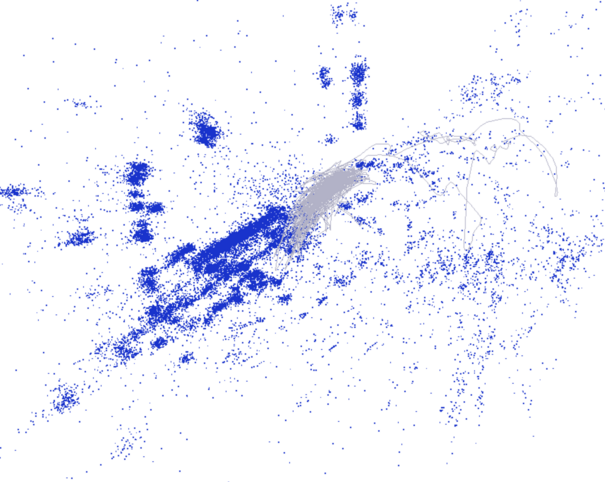
\includegraphics[width=\textwidth]{img/experiments/MIPP01.lc.map.png}
        \caption{BasaltLC}
        \label{fig:mipp01_basaltlc_map}
    \end{subfigure}
    \hfill
    \begin{subfigure}[b]{0.32\textwidth}
        \centering
        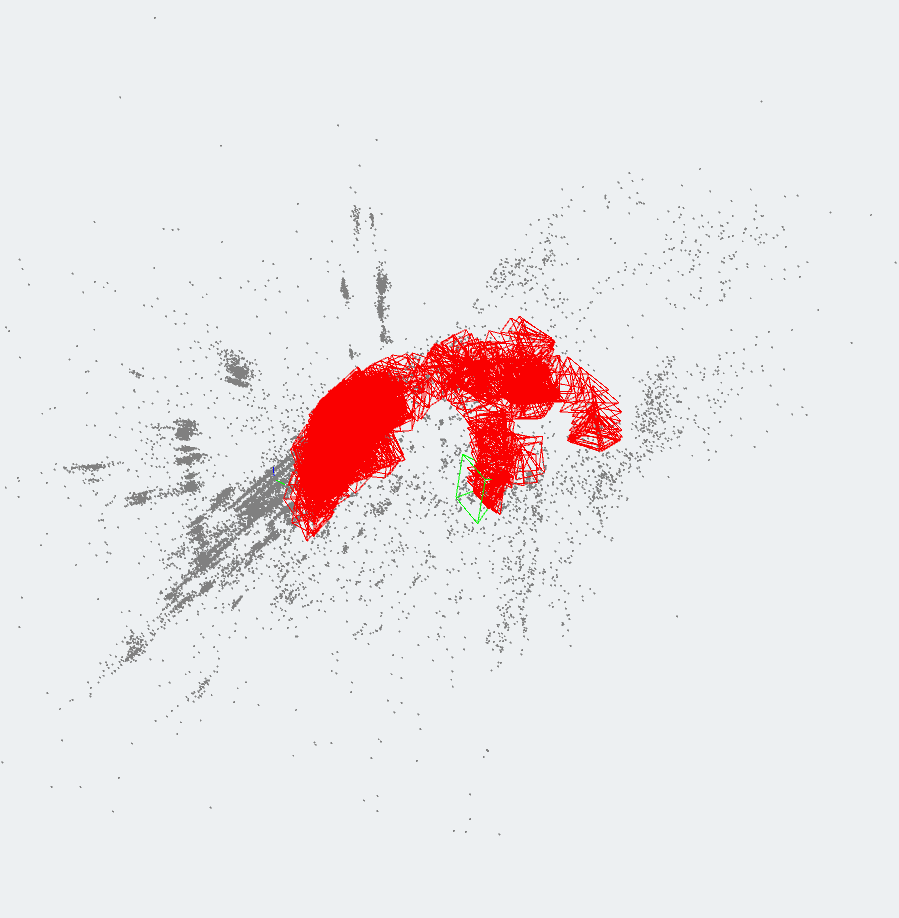
\includegraphics[width=\textwidth]{img/experiments/MIPP01.slam.map.png}
        \caption{BasaltSLAM}
        \label{fig:mipp01_basaltslam_map}
    \end{subfigure}
    \caption{Mapas obtenidos por Basalt, BasaltLC y BasaltSLAM para la secuencia MIPP01.}
    \label{fig:mipp01_ablation_maps}
\end{figure}

\begin{figure}[ht]
    \centering
    \begin{subfigure}[b]{0.32\textwidth}
        \centering
        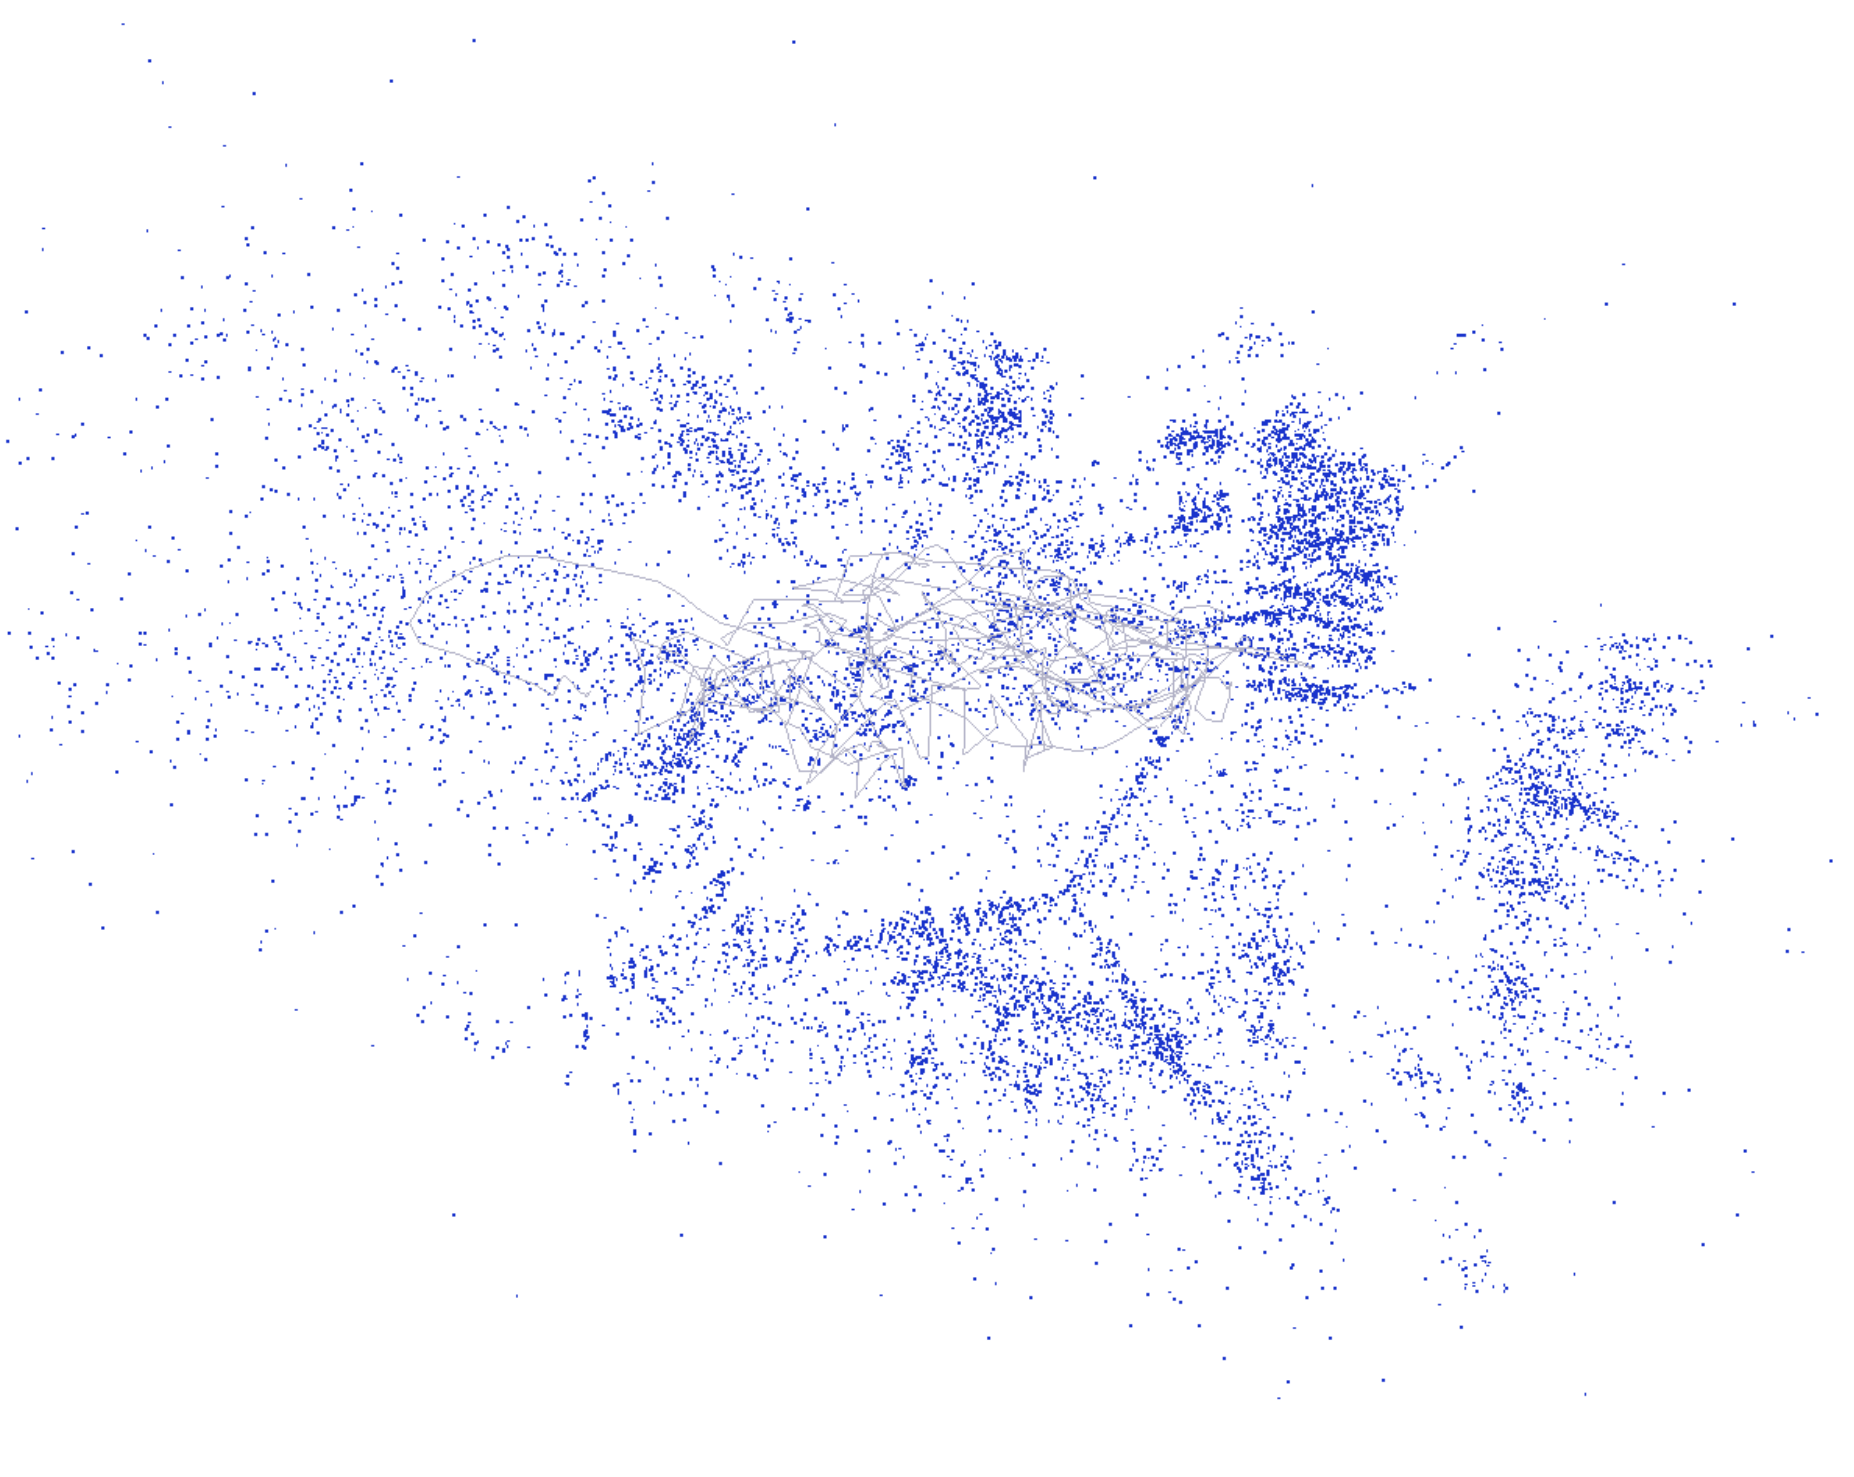
\includegraphics[width=\textwidth]{img/experiments/MGO01.vio.map.png}
        \caption{Basalt}
        \label{fig:mgo01_basalt_map}
    \end{subfigure}
    \hfill
    \begin{subfigure}[b]{0.32\textwidth}
        \centering
        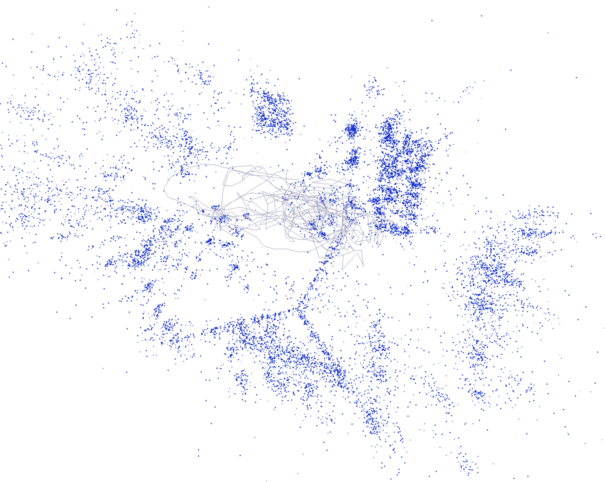
\includegraphics[width=\textwidth]{img/experiments/MGO01.lc.map.png}
        \caption{BasaltLC}
        \label{fig:mgo01_basaltlc_map}
    \end{subfigure}
    \hfill
    \begin{subfigure}[b]{0.32\textwidth}
        \centering
        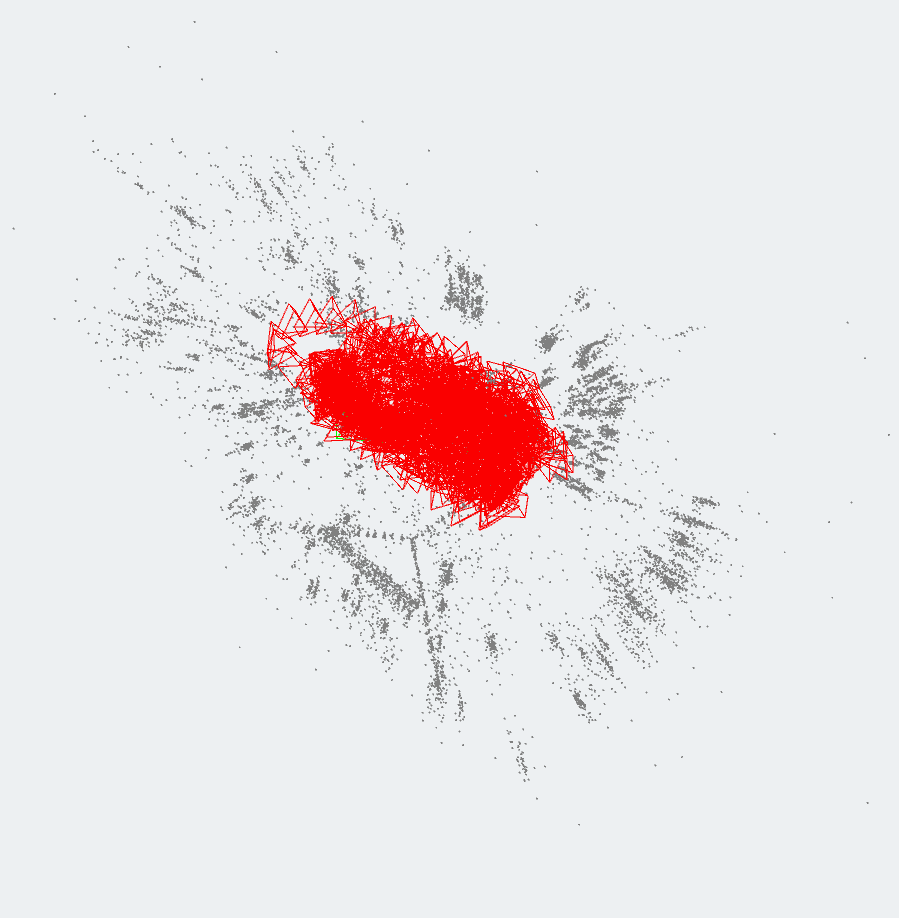
\includegraphics[width=\textwidth]{img/experiments/MGO01.slam.map.png}
        \caption{BasaltSLAM}
        \label{fig:mgo01_basaltslam_map}
    \end{subfigure}
    \caption{Mapas obtenidos por Basalt, BasaltLC y BasaltSLAM para la secuencia MGO01.}
    \label{fig:mgo01_ablation_maps}
\end{figure}

En la Figura \ref{fig:msd_ablation_timings} se muestran los tiempos de procesamiento por frame para cada sistema
en las secuencias de MSD. En este análisis no se incluyó la versión BasaltSLAM, ya que no fue posible representar
el tiempo de ejecución de la optimización final en tales gráficas. Por lo tanto, la performance de RootBA
será analizada en las siguientes secciones.
Se observa que, para los cascos Odyssey+ y HP Reverb G2 V2, tanto BasaltLC como
BasaltLC-CQ mantienen un tiempo de procesamiento por frame por debajo del límite de tiempo para la operación en tiempo real,
aunque muestran un promedio de procesamiento levemente superior a Basalt.
En el caso del Valve Index, BasaltLC obtiene una diferencia de 0.6 ms de promedio en comparación con Basalt. Aún así, su promedio
móvil se mantiene por debajo del límite de tiempo para la operación en tiempo real, con un margen ajustado. Por otro lado,
BasaltLC-CQ muestra un aumento de 5.1 ms de promedio en comparación con Basalt, lo que hace que su promedio móvil supere el
límite de tiempo para la operación en tiempo real.

\begin{figure}[ht]
    \centering
    \begin{subfigure}[b]{0.48\textwidth}
        \centering
        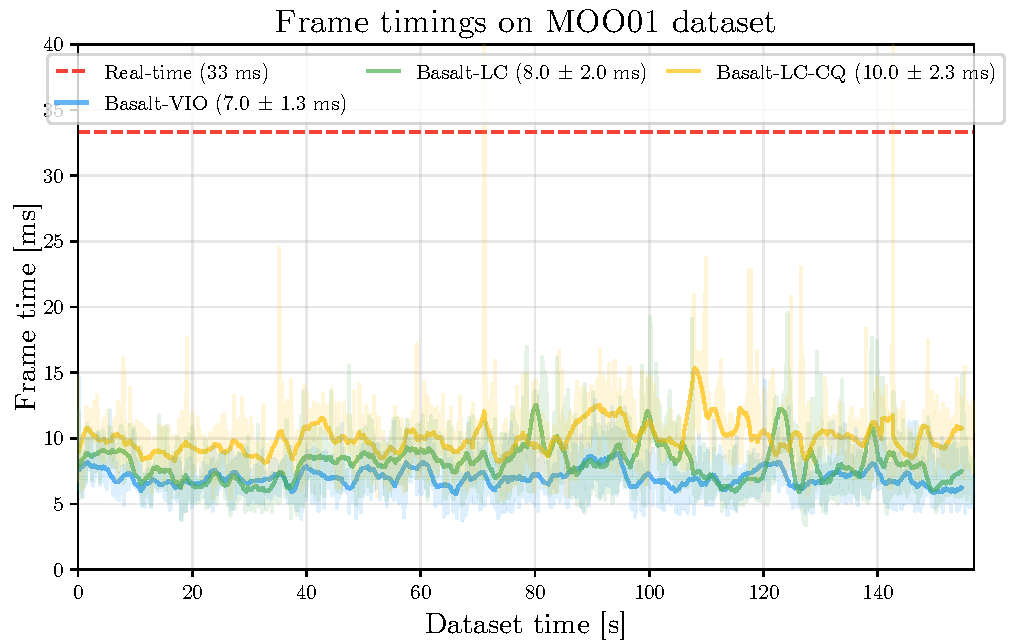
\includegraphics[width=\textwidth]{img/experiments/MOO01.timings.ablation.pdf}
        \caption{Secuencia capturada con Odyssey+.}
        \label{fig:experiments_figure16}
    \end{subfigure}
    \hfill
    \begin{subfigure}[b]{0.48\textwidth}
        \centering
        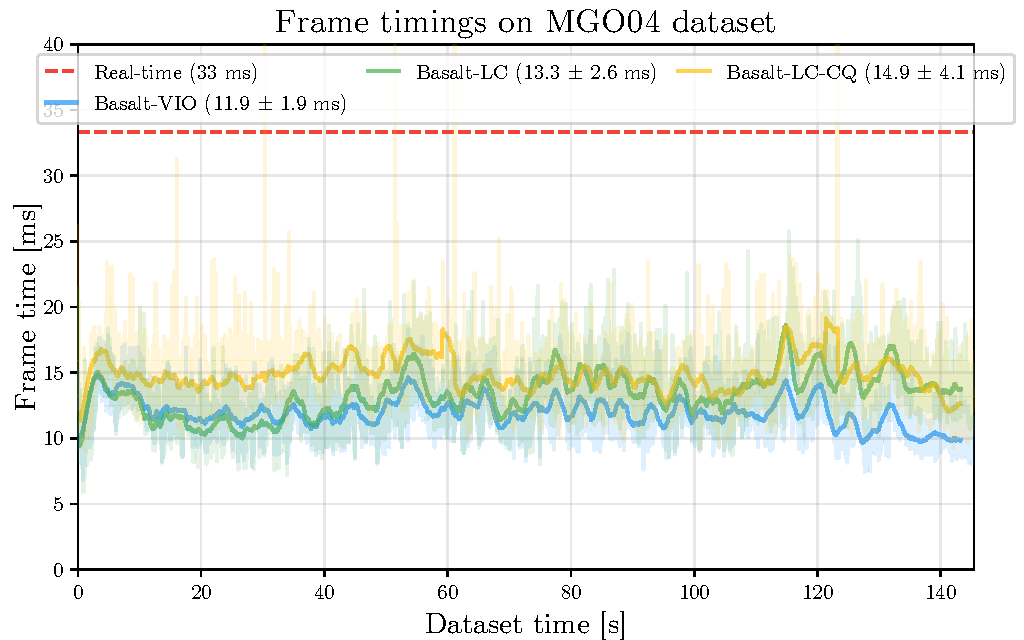
\includegraphics[width=\textwidth]{img/experiments/MGO04.timings.ablation.pdf}
        \caption{Secuencia capturada con HP Reverb G2 V2.}
        \label{fig:experiments_figure17}
    \end{subfigure}
    \hfill
    \begin{subfigure}[b]{0.48\textwidth}
        \centering
        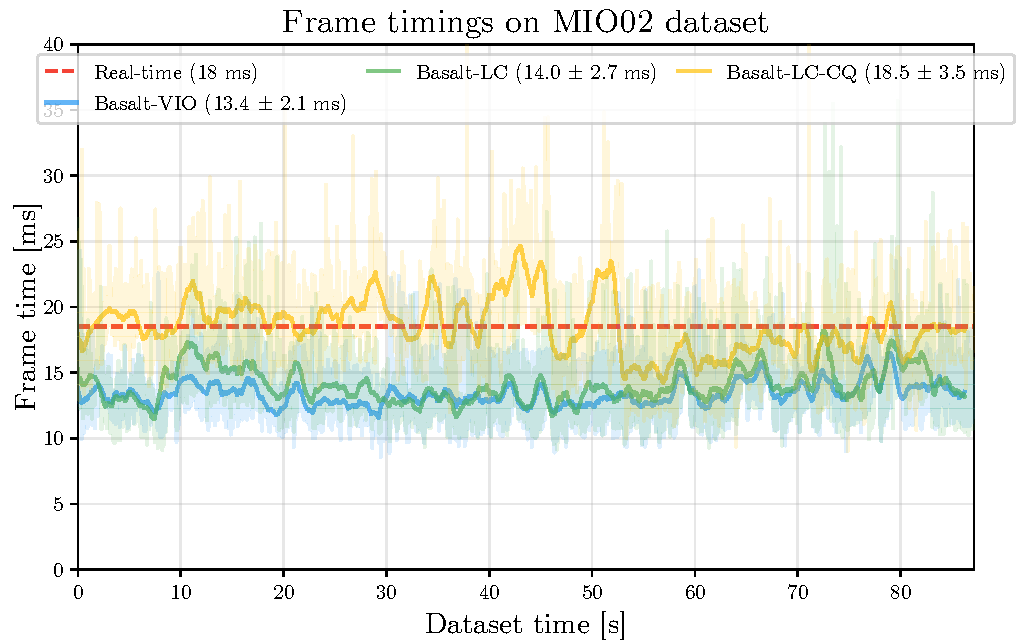
\includegraphics[width=\textwidth]{img/experiments/MIO02.timings.ablation.pdf}
        \caption{Secuencia capturada con Valve Index.}
        \label{fig:experiments_figure18}
    \end{subfigure}
    \caption{Tiempo de procesamiento por frame para cada sistema en las secuencias de MO*, MG* y MI* respectivamente.
    Se muestra un promedio móvil con una ventana de 2 segundos (60 frames). En el fondo, los datos sin procesar muestran
    outliers y jitter para cada sistema. Una línea roja marca el límite de tiempo para la operación en tiempo real para cada headset.
    Nótese que BasaltLC y BasaltLC-CQ se ejecutaron en su versión síncrona, con el mapa asíncrono. Experimento realizado
    en un procesador Intel Core Ultra 9 285H con 32 GB de RAM.}
    \label{fig:msd_ablation_timings}
\end{figure}

En conclusión, BasaltSLAM es el sistema más robusto, logrando la mejor precisión en términos de ATE
y manteniendo una precisión comparable a la de Basalt en RTE. Asimismo, estos resultados se obtienen
sin comprometer la capacidad de operar en tiempo real. En la siguiente sección se compara la performance
y precisión de BasaltSLAM con otros sistemas de VI-SLAM del estado del arte.

\section{BasaltSLAM vs estado del arte}

El objetivo de este experimento es evaluar la performance y precisión de BasaltSLAM en comparación con
otros sistemas del estado del arte. Se eligieron ORB-SLAM3 y OKVIS2 como sistemas de referencia.
Ambos fueron ejecutados en sus versiones SLAM con loop closure y optimización final de bundle adjustment.
Al igual que en el estudio de ablación, se analiza la estimación no causal de la trayectoria y la performance de cada sistema.

La Figura~\ref{fig:sota_trajectories} muestra ejemplos cualitativos de trayectorias para secuencias representativas de los tres datasets.

\begin{figure}[ht]
    \centering
    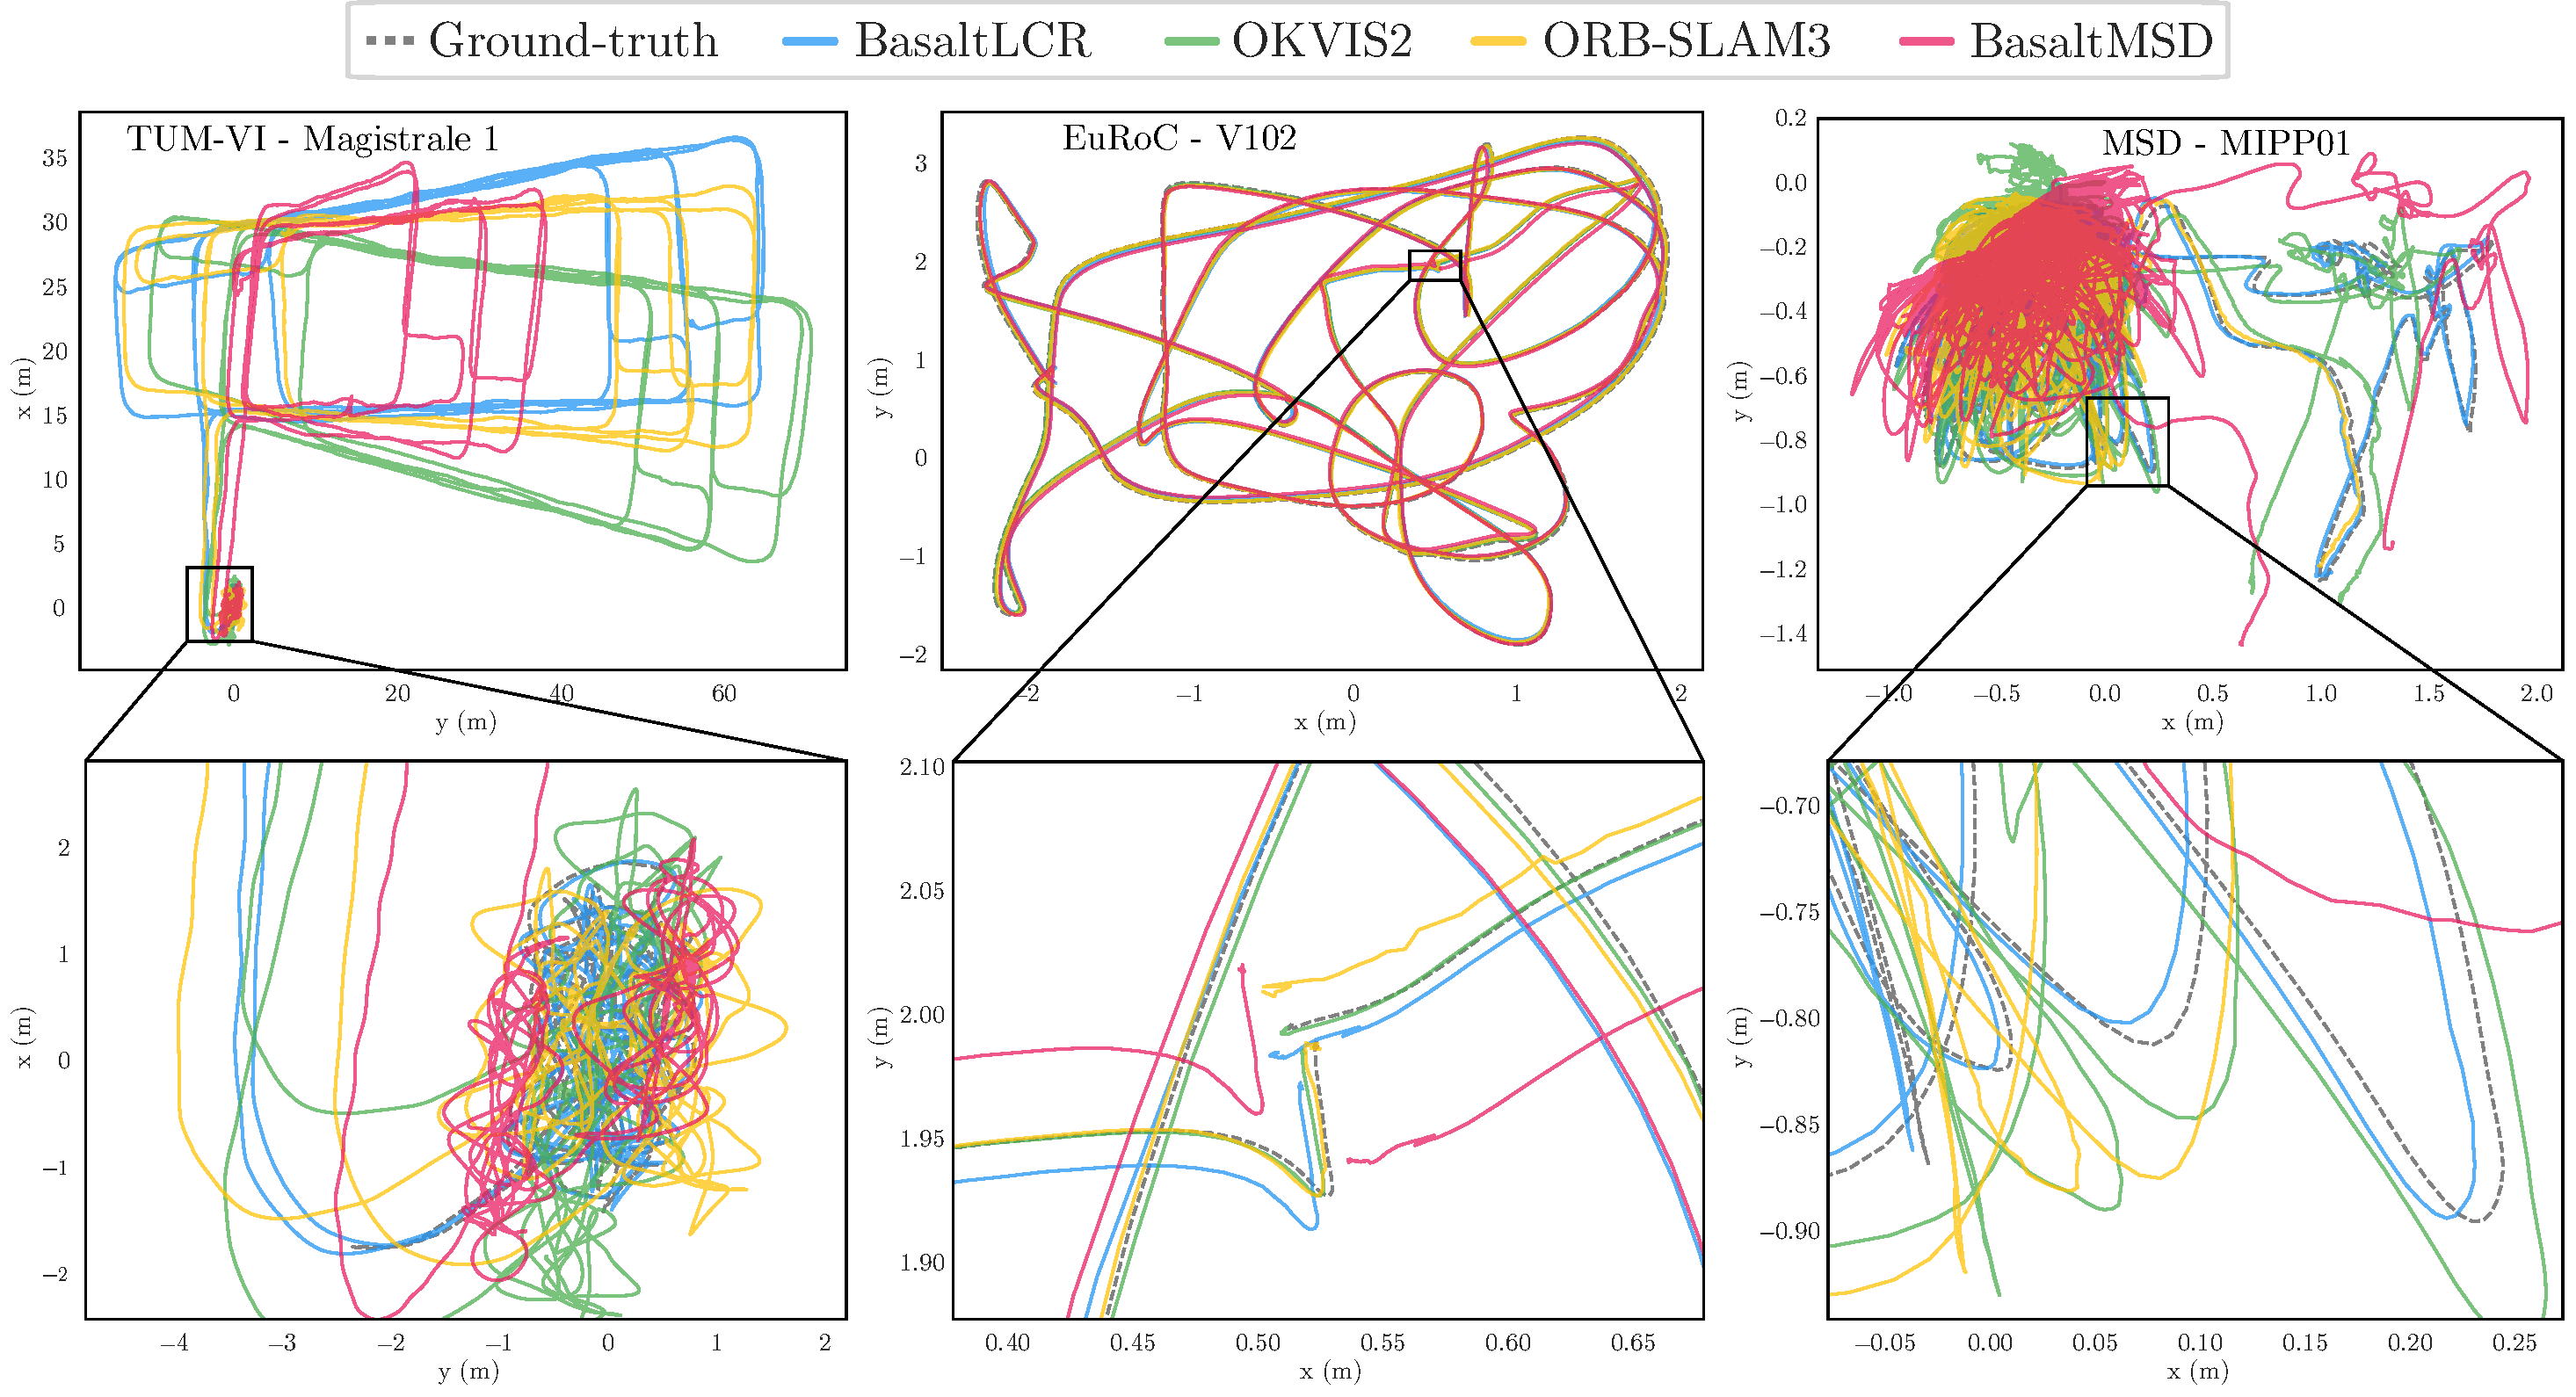
\includegraphics[width=\textwidth]{img/experiments/sota.trajectories.pdf}
    \caption{Ejemplos de trayectorias para secuencias de distintos datasets, con ampliaciones en partes que resultan de interés. Se comparan Basalt en su versión VIO, con el sistema propuesto, y OKVIS2 y ORB-SLAM3 como referencias del estado del arte de VI-SLAM. En Magistrale 1 el sistema propuesto fue el único capaz de detectar el ciclo al reingresar en la habitación. Como se observa en la ampliación de su trayectoria, esta secuencia solo cuenta con ground-truth en la parte de la habitación, al comienzo y al final. En V102, si bien el método propuesto mejora la estimación del VIO de Basalt, no alcanza la precisión de OKVIS2 y ORB-SLAM3. Por último, en MIPP01, el método propuesto es el único capaz de mantener el drift acotado durante toda la secuencia. Tanto OKVIS2 como Basalt acumulan drift considerable, evidenciado por la gran separación entre el inicio y el fin de sus trayectorias. ORB-SLAM3 no es capaz de mantener el tracking y consigue estimar solo el 85\% del total de la secuencia.}
    \label{fig:sota_trajectories}
\end{figure}

Primero, se presentarán los resultados en los datasets del estado del arte. Luego, se finalizará con los resultados en las
secuencias de MSD, en las que además se analizará la performance y robustez.

\subsection{Resultados en datasets del estado del arte}

En la Tabla \ref{tab:corridor_sota_ate} se muestran los resultados de ATE para las secuencias ``Corridor''.
Se observa que BasaltSLAM obtiene resultados levemente mejores que OKVIS2, y ORB-SLAM3 obtiene los mejores resultados.

\begin{table}[ht]
\centering
\caption{Error de trayectoria absoluto (ATE) [m] en TUM-VI Corridor.}
\label{tab:corridor_sota_ate}
\begin{tabular}{lrrr}
\toprule
\textbf{Dataset} & \textbf{BasaltSLAM} & \textbf{OKVIS2} & \textbf{ORB-SLAM3} \\
\midrule
TC1 & \textbf{0.03} & 0.09 & \textbf{0.03} \\
TC2 & 0.07 & 0.06 & \textbf{0.02} \\
TC3 & 0.06 & \textbf{0.02} & \textbf{0.02} \\
TC4 & 0.22 & \textbf{0.18} & 0.21 \\
TC5 & 0.03 & 0.09 & \textbf{0.01} \\
\midrule
Median & 0.06 & 0.09 & \textbf{0.02} \\
Mean & 0.08 & 0.09 & \textbf{0.06} \\
\bottomrule
\end{tabular}
\end{table}

En la Tabla \ref{tab:magistrale_sota_ate} se muestran los resultados de ATE para las secuencias ``Magistrale''.
En este caso, OKVIS2 consigue detectar ciclos más consistentemente y obtiene resultados significativamente mejores
que BasaltSLAM y ORB-SLAM3.
Sin embargo, en TM6 BasaltSLAM es capaz de detectar ciclos que ninguno de los otros sistemas pudo detectar, obteniendo
un resultado considerablemente mejor.

\begin{table}[ht]
\centering
\caption{Error de trayectoria absoluto (ATE) [m] en TUM-VI Magistrale.}
\label{tab:magistrale_sota_ate}
\begin{tabular}{lrrr}
\toprule
\textbf{Dataset} & \textbf{BasaltSLAM} & \textbf{OKVIS2} & \textbf{ORB-SLAM3} \\
\midrule
TM1 & 0.07 & \textbf{0.03} & 0.24 \\
TM2 & 0.87 & \textbf{0.03} & 0.52 \\
TM3 & 1.66 & \textbf{0.93} & 1.86 \\
TM4 & 1.51 & \textbf{0.04} & 0.16 \\
TM5 & 0.95 & \textbf{0.01} & 1.13 \\
TM6 & \textbf{0.02} & 0.63 & 0.97 \\
\midrule
Median & 0.91 & \textbf{0.04} & 0.74 \\
Mean & 0.85 & \textbf{0.28} & 0.81 \\
\bottomrule
\end{tabular}
\end{table}

En la Tabla \ref{tab:outdoors_sota_ate} se muestran los resultados de ATE para las secuencias ``Outdoors''.
En este caso, todos los sistemas presentan dificultades para detectar ciclos, aunque OKVIS2 destaca en las secuencias
TO2, TO7 y TO8 donde consigue detectar ciclos importantes, obteniendo resultados notablemente superiores a los
de BasaltSLAM y ORB-SLAM3. Para entender mejor lo que ocurre en estas secuencias, la grabación comienza
capturando una mitad de una habitación, luego se sale de esta, haciendo un recorrido por el exterior
y finalmente se reingresa nuevamente en la misma habitación, capturando la otra mitad. Los ciclos más significativos
que consiguen reducir el ATE se dan al reentrar en la misma habitación, pero como captura la pared contraria,
existe una intersección pequeña entre la escena del comienzo y la del final, lo que hace que sea difícil de detectar para los sistemas.

La Figura \ref{fig:to2_hard_loop} muestra un ejemplo de BasaltSLAM en el que se redujeron los parámetros de detección,
exigiendo solo 10 inliers para validar un ciclo. Esto permitió detectar uno de estos ciclos con baja intersección,
pero también generó un gran número de falsos positivos. Este comportamiento puede ser indicativo de la superioridad de OKVIS2,
el cual requiere solo 10 inliers para la detección pero compensa con un mayor número de verificaciones geométricas
para descartar falsos positivos.

\begin{table}[ht]
\centering
\caption{Error de trayectoria absoluto (ATE) [m] en TUM-VI Outdoors.}
\label{tab:outdoors_sota_ate}
\begin{tabular}{lrrr}
\toprule
\textbf{Dataset} & \textbf{BasaltSLAM} & \textbf{OKVIS2} & \textbf{ORB-SLAM3} \\
\midrule
TO1 & 284.24 & \textbf{24.92} & 32.32 \\
TO2 & 60.45 & \textbf{0.04} & 10.42 \\
TO3 & 34.92 & \textbf{27.14} & 54.77 \\
TO4 & 14.07 & \textbf{7.42} & 11.61 \\
TO5 & 12.62 & \textbf{6.67} & 7.57 \\
TO6 & 77.55 & 26.37 & \textbf{10.70} \\
TO7 & 2.07 & \textbf{0.15} & 4.58 \\
TO8 & 12.15 & \textbf{0.05} & 11.02 \\
\midrule
Median & 24.50 & \textbf{7.04} & 10.86 \\
Mean & 62.26 & \textbf{11.60} & 17.87 \\
\bottomrule
\end{tabular}
\end{table}

\begin{figure}[ht]
    \centering
    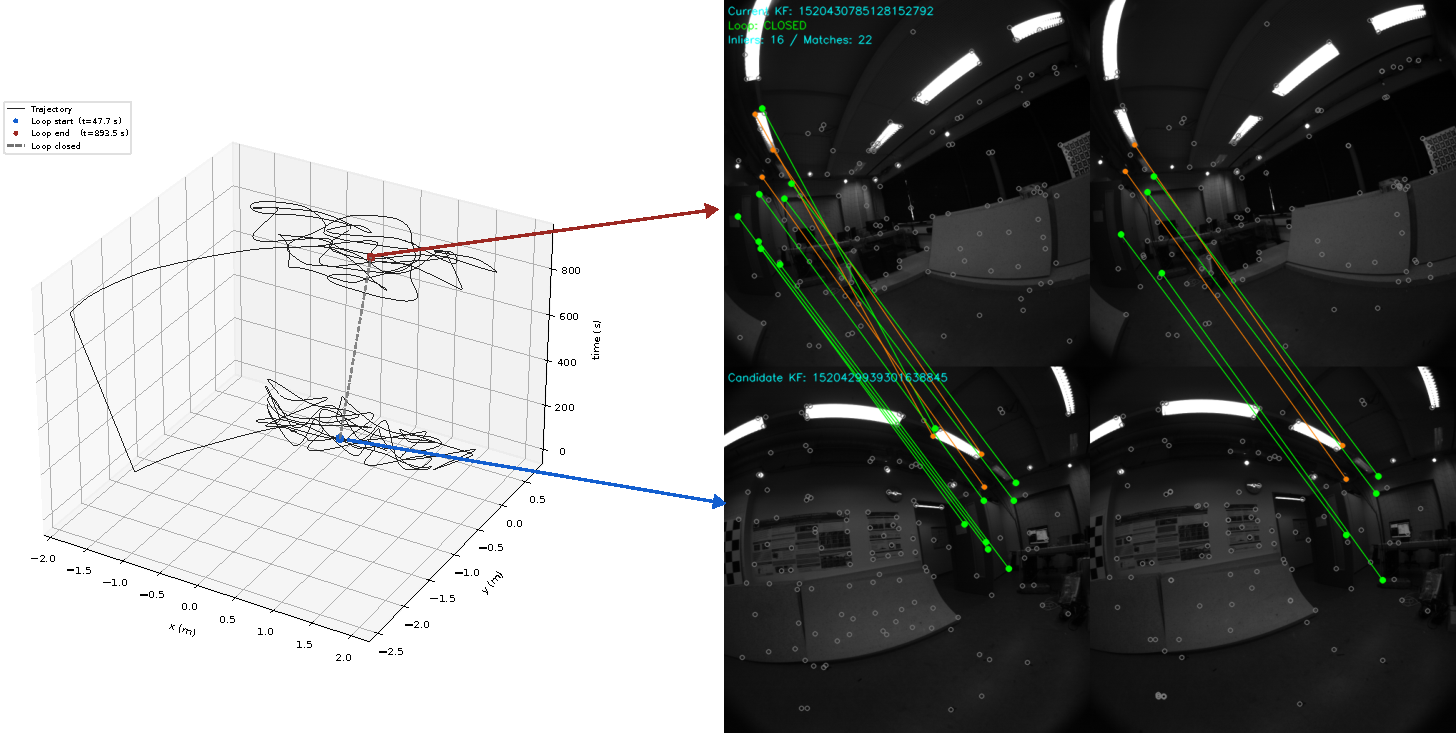
\includegraphics[width=0.8\textwidth]{img/experiments/TO2.hard_loop.pdf}
    \caption{Ciclo detectado en la secuencia TO2, con una intersección pequeña entre la escena del comienzo y la del final.
    Para detectar este ciclo, se redujeron los parámetros de detección de BasaltSLAM, necesitando solo 10 inliers.
    Se dibuja la trayectoria ground truth, en vez de la estimada, pues esta tuvo un gran número de falsos positivos que la corrompieron.}
    \label{fig:to2_hard_loop}
\end{figure}


En la Tabla \ref{tab:room_sota_ate} se muestran los resultados de ATE para las secuencias ``Room''.
En este caso, todos los sistemas se encuentran al mismo nivel, con una precisión milimétrica.

\begin{table}[ht]
\centering
\caption{Error de trayectoria absoluto (ATE) [m] en TUM-VI Room.}
\label{tab:room_sota_ate}
\begin{tabular}{lrrr}
\toprule
\textbf{Dataset} & \textbf{BasaltSLAM} & \textbf{OKVIS2} & \textbf{ORB-SLAM3} \\
\midrule
TR1 & \textbf{0.01} & \textbf{0.01} & \textbf{0.01} \\
TR2 & \textbf{0.01} & \textbf{0.01} & \textbf{0.01} \\
TR3 & \textbf{0.01} & \textbf{0.01} & \textbf{0.01} \\
TR4 & \textbf{0.01} & \textbf{0.01} & \textbf{0.01} \\
TR5 & \textbf{0.01} & \textbf{0.01} & \textbf{0.01} \\
TR6 & \textbf{0.01} & \textbf{0.01} & \textbf{0.01} \\
\midrule
Median & \textbf{0.01} & \textbf{0.01} & \textbf{0.01} \\
Mean & \textbf{0.01} & \textbf{0.01} & \textbf{0.01} \\
\bottomrule
\end{tabular}
\end{table}


En la Tabla \ref{tab:slides_sota_ate} se muestran los resultados de ATE para las secuencias ``Slides''.
En este caso, BasaltSLAM obtiene resultados superiores para la secuencia TS1, pero OKVIS2 y ORB-SLAM3 obtienen mejores resultados
en las secuencias TS2 y TS3 respectivamente.

\begin{table}[ht]
\centering
\caption{Error de trayectoria absoluto (ATE) [m] en TUM-VI Slides.}
\label{tab:slides_sota_ate}
\begin{tabular}{lrrr}
\toprule
\textbf{Dataset} & \textbf{BasaltSLAM} & \textbf{OKVIS2} & \textbf{ORB-SLAM3} \\
\midrule
TS1 & \textbf{0.01} & 0.10 & 0.41 \\
TS2 & 1.23 & \textbf{0.16} & 0.49 \\
TS3 & 1.51 & 1.35 & \textbf{0.47} \\
\midrule
Median & 1.23 & \textbf{0.16} & 0.47 \\
Mean & 0.92 & 0.54 & \textbf{0.46} \\
\bottomrule
\end{tabular}
\end{table}

En la Tabla \ref{tab:MH_sota_ate} se muestran los resultados de ATE para las secuencias de ``Machine Hall''.
OKVIS2 domina en este caso, obteniendo resultados notablemente mejores que BasaltSLAM. ORB-SLAM3 se posiciona
entre ambos sistemas.

\begin{table}[ht]
\centering
\caption{Error de trayectoria absoluto (ATE) [m] en EuRoC Machine Hall.}
\label{tab:MH_sota_ate}
\begin{tabular}{lrrr}
\toprule
\textbf{Dataset} & \textbf{BasaltSLAM} & \textbf{OKVIS2} & \textbf{ORB-SLAM3} \\
\midrule
EMH01 & 0.08 & \textbf{0.03} & 0.04 \\
EMH02 & 0.05 & \textbf{0.02} & 0.03 \\
EMH03 & 0.05 & \textbf{0.03} & 0.04 \\
EMH04 & 0.13 & 0.07 & \textbf{0.05} \\
EMH05 & 0.09 & \textbf{0.07} & 0.08 \\
\midrule
Median & 0.08 & \textbf{0.03} & 0.04 \\
Mean & 0.08 & \textbf{0.04} & 0.05 \\
\bottomrule
\end{tabular}
\end{table}

En la Tabla \ref{tab:V1_sota_ate} se muestran los resultados de ATE para las secuencias de ``Vicon Room 1''.
En este caso, BasaltSLAM iguala los resultados de OKVIS2 y ORB-SLAM3 en EV101, pero en las secuencias EV102
y EV103, OKVIS2 y ORB-SLAM3 consiguen resultados superiores a BasaltSLAM. Resultados similares
se obtienen en la Tabla \ref{tab:V2_sota_ate} para las secuencias de ``Vicon Room 2''.

\begin{table}[ht]
\centering
\caption{Error de trayectoria absoluto (ATE) [m] en EuRoC Vicon Room 1.}
\label{tab:V1_sota_ate}
\begin{tabular}{lrrr}
\toprule
\textbf{Dataset} & \textbf{BasaltSLAM} & \textbf{OKVIS2} & \textbf{ORB-SLAM3} \\
\midrule
EV101 & \textbf{0.04} & \textbf{0.04} & \textbf{0.04} \\
EV102 & 0.03 & \textbf{0.01} & \textbf{0.01} \\
EV103 & 0.13 & \textbf{0.02} & \textbf{0.02} \\
\midrule
Median & 0.04 & \textbf{0.02} & \textbf{0.02} \\
Mean & 0.07 & \textbf{0.02} & 0.03 \\
\bottomrule
\end{tabular}
\end{table}

\begin{table}[ht]
\centering
\caption{Error de trayectoria absoluto (ATE) [m] en EuRoC Vicon Room 2.}
\label{tab:V2_sota_ate}
\begin{tabular}{lrrr}
\toprule
\textbf{Dataset} & \textbf{BasaltSLAM} & \textbf{OKVIS2} & \textbf{ORB-SLAM3} \\
\midrule
EV201 & 0.04 & \textbf{0.02} & 0.03 \\
EV202 & 0.10 & \textbf{0.01} & \textbf{0.01} \\
EV203 & 0.14 & \textbf{0.02} & \textbf{0.02} \\
\midrule
Median & 0.10 & \textbf{0.02} & \textbf{0.02} \\
Mean & 0.09 & \textbf{0.02} & \textbf{0.02} \\
\bottomrule
\end{tabular}
\end{table}


\subsection{Resultados en datasets de XR}

En la Tabla \ref{tab:msdmi_sota_all} se muestran los resultados de ATE, RTE y porcentaje de secuencia completada de MI*.
OKVIS2 obtiene la mejor mediana tanto en ATE como en RTE, aunque BasaltSLAM se sitúa apenas 0.3 y 0.2 cm por encima
respectivamente. Además, BasaltSLAM demuestra mayor robustez, lo cual se refleja en que obtiene el mejor promedio de ATE y RTE.
ORB-SLAM3 presenta resultados inferiores en ambas métricas y no logra completar un gran número de secuencias.

\begin{table}[ht]
\centering
\caption{ATE [cm], RTE [cm] y tasa de completitud (\%) en MSD Valve Index.}
\label{tab:msdmi_sota_all}
\begin{tabular}{l rrr | rrr | rrr}
\toprule
& \multicolumn{3}{c|}{\textbf{ATE [cm]}} & \multicolumn{3}{c|}{\textbf{RTE [cm]}} & \multicolumn{3}{c}{\textbf{Completitud (\%)}} \\
\cmidrule(lr){2-4} \cmidrule(lr){5-7} \cmidrule(lr){8-10}
\textbf{Secuencia}
& \rotatebox{90}{\textbf{BasaltSLAM}\,}
& \rotatebox{90}{\textbf{OKVIS2}\,}
& \rotatebox{90}{\textbf{ORB-SLAM3}\,}
& \rotatebox{90}{\textbf{BasaltSLAM}\,}
& \rotatebox{90}{\textbf{OKVIS2}\,}
& \rotatebox{90}{\textbf{ORB-SLAM3}\,}
& \rotatebox{90}{\textbf{BasaltSLAM}\,}
& \rotatebox{90}{\textbf{OKVIS2}\,}
& \rotatebox{90}{\textbf{ORB-SLAM3}\,} \\
\midrule
MIO01   & \textbf{18.7} & 6912.6 & 56928.9 & \textbf{4.4} & 82.3  & 366.4 & \textbf{100} & \textbf{100} & 69 \\
MIO02   & 23.6          & 146.7  & \textbf{6.8}    & 4.0          & 3.1   & \textbf{1.5}  & \textbf{100} & \textbf{100} & 27 \\
MIO03   & \textbf{2.5}  & 4.4    & 3.7             & 1.0          & \textbf{0.7}  & 1.0  & \textbf{100} & \textbf{100} & 82 \\
MIO04   & \textbf{7.4}  & 16.7   & 106.4           & 3.6          & \textbf{1.1}  & 39.4 & \textbf{100} & \textbf{100} & 95 \\
MIO05   & \textbf{1.9}  & 2.4    & 2.0             & \textbf{0.3} & 1.2   & 0.8  & \textbf{100} & \textbf{100} & 78 \\
MIO06   & \textbf{2.6}  & 6.4    & 31.7            & \textbf{1.4} & 1.6   & 11.3 & \textbf{100} & \textbf{100} & \textbf{100} \\
MIO07   & 1.2           & 1.6    & \textbf{1.1}    & \textbf{0.2} & 0.6   & 0.6  & \textbf{100} & \textbf{100} & 59 \\
MIO08   & 6.9           & 3.5    & \textbf{2.0}    & 3.9          & \textbf{0.6}  & 0.8  & \textbf{100} & \textbf{100} & 97 \\
MIO09   & \textbf{0.2}  & 0.7    & 0.4             & \textbf{0.2} & 0.5   & 0.4  & \textbf{100} & 99  & 90 \\
MIO10   & 1.8           & \textbf{1.5}    & --     & 0.6          & \textbf{0.5}  & --   & \textbf{100} & \textbf{100} & -- \\
MIO11   & \textbf{2.3}  & 2.7    & --              & \textbf{0.6} & \textbf{0.6}  & --   & \textbf{100} & \textbf{100} & -- \\
MIO12   & \textbf{4.2}  & 60.5   & 1141.6          & 0.6          & \textbf{0.5}  & 221.3 & \textbf{100} & \textbf{100} & 95 \\
MIO13   & \textbf{28.0} & 35.6   & 109055.1        & 2.7          & \textbf{0.6}  & 505.2 & \textbf{100} & \textbf{100} & 30 \\
MIO14   & \textbf{2.5}  & 2.7    & --              & \textbf{0.3} & 0.4   & --   & \textbf{100} & \textbf{100} & -- \\
MIO15   & 10.7          & 13.3   & \textbf{3.0}    & 1.3          & \textbf{0.5}  & 1.4  & \textbf{100} & \textbf{100} & 37 \\
MIO16   & 18.7          & 15.2   & \textbf{1.7}    & 2.5          & 0.9   & \textbf{0.4}  & \textbf{100} & \textbf{100} & 31 \\
MIPB01  & 1.3           & 1.7    & \textbf{1.2}    & 0.6          & \textbf{0.5}  & 0.7  & \textbf{100} & \textbf{100} & 99 \\
MIPB02  & 3.5           & 2.0    & \textbf{1.4}    & 2.7          & \textbf{0.5}  & 0.6  & \textbf{100} & \textbf{100} & 99 \\
MIPB03  & \textbf{2.9}  & 5.2    & 9.1             & 0.7          & \textbf{0.5}  & 1.1  & \textbf{100} & \textbf{100} & 99 \\
MIPB04  & 2.0           & 2.4    & \textbf{1.6}    & 0.6          & \textbf{0.4}  & 0.6  & \textbf{100} & \textbf{100} & 97 \\
MIPB05  & \textbf{1.4}  & 2.1    & 1.9             & 0.5          & \textbf{0.4}  & 0.6  & \textbf{100} & \textbf{100} & 80 \\
MIPB06  & 2.9           & 1.9    & \textbf{1.5}    & \textbf{0.5} & \textbf{0.5}  & 0.6  & \textbf{100} & \textbf{100} & 83 \\
MIPB07  & 1.6           & 1.8    & \textbf{1.3}    & 0.5          & \textbf{0.4}  & 0.6  & \textbf{100} & \textbf{100} & 79 \\
MIPB08  & 3.9           & \textbf{3.6}    & 25.9   & 0.5          & \textbf{0.4}  & 1.0  & \textbf{100} & \textbf{100} & 96 \\
MIPP01  & \textbf{2.9}  & 10.1   & 24.4            & 1.1          & \textbf{0.5}  & 5.8  & \textbf{100} & \textbf{100} & 78 \\
MIPP02  & 3.9           & \textbf{1.8}    & 4.2    & 1.7          & \textbf{0.4}  & 1.7  & \textbf{100} & \textbf{100} & 57 \\
MIPP03  & 4.8           & \textbf{2.3}    & 6.3    & 2.3          & \textbf{0.5}  & 5.8  & \textbf{100} & \textbf{100} & 65 \\
MIPP04  & 2.5           & \textbf{1.1}    & 1.7    & 1.0          & \textbf{0.4}  & 0.9  & \textbf{100} & \textbf{100} & 74 \\
MIPP05  & 2.7           & 1.5    & \textbf{1.2}    & 1.9          & \textbf{0.4}  & 0.6  & \textbf{100} & \textbf{100} & 99 \\
MIPP06  & 2.7           & \textbf{1.2}    & 87.7   & 1.2          & \textbf{0.4}  & 2.8  & \textbf{100} & \textbf{100} & 98 \\
MIPT01  & 1.7           & 1.9    & \textbf{1.5}    & 0.5          & \textbf{0.4}  & 0.6  & \textbf{100} & \textbf{100} & \textbf{100} \\
MIPT02  & 2.1           & 2.0    & \textbf{1.1}    & 0.5          & \textbf{0.4}  & 0.6  & \textbf{100} & \textbf{100} & 98 \\
MIPT03  & \textbf{3.5}  & 4.6    & 34.4            & \textbf{0.6} & \textbf{0.6}  & 2.7  & \textbf{100} & \textbf{100} & 96 \\
\midrule
Mediana & 2.7           & \textbf{2.4}    & 2.5    & 0.7          & \textbf{0.5}  & 0.9  & \textbf{100} & \textbf{100} & 86 \\
Promedio & \textbf{5.4} & 220.4  & 5583.0          & \textbf{1.4} & 3.1   & 39.3 & \textbf{100} & \textbf{100} & 80 \\
\bottomrule
\end{tabular}
\end{table}

En la Tabla \ref{tab:msdmg_sota_all} se muestran los resultados de ATE, RTE y porcentaje de secuencia completada de MG*.
Se observa un comportamiento similar al de MI*: OKVIS2 obtiene la mejor mediana tanto en ATE como en RTE,
pero BasaltSLAM logra valores competitivos en ambas métricas y la mayor precisión en términos de promedio. ORB-SLAM3
queda por detrás en ambas métricas y no consigue completar un número considerable de secuencias.

\begin{table}[ht]
\centering
\caption{ATE [cm], RTE [cm] y tasa de completitud (\%) en MSD HP Reverb G2.}
\label{tab:msdmg_sota_all}
\begin{tabular}{l rrr | rrr | rrr}
\toprule
& \multicolumn{3}{c|}{\textbf{ATE [cm]}} & \multicolumn{3}{c|}{\textbf{RTE [cm]}} & \multicolumn{3}{c}{\textbf{Completitud (\%)}} \\
\cmidrule(lr){2-4} \cmidrule(lr){5-7} \cmidrule(lr){8-10}
\textbf{Secuencia}
& \rotatebox{90}{\textbf{BasaltSLAM}\,}
& \rotatebox{90}{\textbf{OKVIS2}\,}
& \rotatebox{90}{\textbf{ORB-SLAM3}\,}
& \rotatebox{90}{\textbf{BasaltSLAM}\,}
& \rotatebox{90}{\textbf{OKVIS2}\,}
& \rotatebox{90}{\textbf{ORB-SLAM3}\,}
& \rotatebox{90}{\textbf{BasaltSLAM}\,}
& \rotatebox{90}{\textbf{OKVIS2}\,}
& \rotatebox{90}{\textbf{ORB-SLAM3}\,} \\
\midrule
MGO01 & 12.1 & 18.5 & \textbf{1.8} & 2.4 & \textbf{1.0} & 1.4 & \textbf{100} & \textbf{100} & \textbf{100} \\
MGO02 & 7.5 & \textbf{7.0} & 38.0 & 3.1 & \textbf{1.7} & 2.0 & \textbf{100} & \textbf{100} & 83 \\
MGO03 & \textbf{1.7} & 1.8 & 1.8 & 1.1 & \textbf{0.8} & 1.1 & \textbf{100} & \textbf{100} & 98 \\
MGO04 & 5.4 & 3.6 & \textbf{2.4} & 2.8 & \textbf{1.0} & 1.6 & \textbf{100} & \textbf{100} & 98 \\
MGO05 & 1.7 & 1.3 & \textbf{1.1} & \textbf{0.3} & 0.4 & 0.7 & \textbf{100} & \textbf{100} & 83 \\
MGO06 & 4.1 & \textbf{2.4} & 3.2 & 1.6 & \textbf{1.1} & 1.9 & \textbf{100} & \textbf{100} & 98 \\
MGO07 & 1.4 & \textbf{0.9} & 1.9 & \textbf{0.4} & 0.5 & 1.0 & \textbf{100} & \textbf{100} & 98 \\
MGO08 & 5.0 & \textbf{1.6} & -- & 3.5 & \textbf{1.1} & -- & \textbf{100} & \textbf{100} & -- \\
MGO09 & 1.1 & \textbf{0.6} & 1.8 & 0.7 & \textbf{0.5} & 1.7 & \textbf{100} & 99 & 92 \\
MGO10 & 1.4 & \textbf{0.7} & 6.0 & \textbf{0.3} & \textbf{0.3} & 1.9 & \textbf{100} & \textbf{100} & 97 \\
MGO11 & \textbf{1.0} & \textbf{1.0} & 5.5 & \textbf{0.4} & \textbf{0.4} & 2.0 & \textbf{100} & \textbf{100} & 98 \\
MGO12 & 5.4 & \textbf{2.7} & 66.7 & 1.7 & \textbf{1.6} & 11.3 & \textbf{100} & \textbf{100} & \textbf{100} \\
MGO13 & \textbf{8.6} & 60.5 & 11397.0 & 4.1 & \textbf{1.8} & 131.0 & \textbf{100} & \textbf{100} & 99 \\
MGO14 & 1.9 & \textbf{1.5} & 2.0 & \textbf{0.9} & \textbf{0.9} & 1.2 & \textbf{100} & \textbf{100} & 99 \\
MGO15 & \textbf{1.9} & 53.8 & 23.9 & \textbf{0.3} & 0.5 & 0.4 & \textbf{100} & \textbf{100} & \textbf{100} \\
\midrule
Mediana & 1.9 & \textbf{1.8} & 2.8 & 1.1 & \textbf{0.9} & 1.6 & \textbf{100} & \textbf{100} & 98 \\
Promedio & \textbf{4.0} & 10.5 & 825.2 & 1.6 & \textbf{0.9} & 11.4 & \textbf{100} & \textbf{100} & 96 \\
\bottomrule
\end{tabular}
\end{table}

En la Tabla \ref{tab:msdmo_sota_all} se muestran los resultados de ATE, RTE y porcentaje de secuencia completada de MO*.
En este caso, ORB-SLAM3 resulta más competitivo, aunque nuevamente no logra completar la totalidad de frames en
todas las secuencias. BasaltSLAM obtiene el menor ATE promedio, mientras que OKVIS2 logra mayor precisión en RTE.

\begin{table}[ht]
\centering
\caption{ATE [cm], RTE [cm] y tasa de completitud (\%) en MSD Samsung Odyssey+.}
\label{tab:msdmo_sota_all}
\begin{tabular}{l rrr | rrr | rrr}
\toprule
& \multicolumn{3}{c|}{\textbf{ATE [cm]}} & \multicolumn{3}{c|}{\textbf{RTE [cm]}} & \multicolumn{3}{c}{\textbf{Completitud (\%)}} \\
\cmidrule(lr){2-4} \cmidrule(lr){5-7} \cmidrule(lr){8-10}
\textbf{Secuencia}
& \rotatebox{90}{\textbf{BasaltSLAM}\,}
& \rotatebox{90}{\textbf{OKVIS2}\,}
& \rotatebox{90}{\textbf{ORB-SLAM3}\,}
& \rotatebox{90}{\textbf{BasaltSLAM}\,}
& \rotatebox{90}{\textbf{OKVIS2}\,}
& \rotatebox{90}{\textbf{ORB-SLAM3}\,}
& \rotatebox{90}{\textbf{BasaltSLAM}\,}
& \rotatebox{90}{\textbf{OKVIS2}\,}
& \rotatebox{90}{\textbf{ORB-SLAM3}\,} \\
\midrule
MOO01 & 3.4 & 2.3 & \textbf{1.5} & 1.7 & \textbf{1.2} & 1.3 & \textbf{100} & \textbf{100} & 99 \\
MOO02 & 5.0 & 2.0 & \textbf{1.6} & 3.1 & \textbf{1.2} & 1.4 & \textbf{100} & \textbf{100} & 99 \\
MOO03 & 3.7 & 10.3 & \textbf{1.6} & 1.2 & \textbf{1.0} & 1.3 & \textbf{100} & \textbf{100} & 99 \\
MOO04 & 4.2 & 2.6 & \textbf{2.0} & 1.6 & \textbf{1.0} & 1.6 & \textbf{100} & \textbf{100} & 97 \\
MOO05 & 1.2 & 1.6 & \textbf{1.1} & \textbf{0.3} & 0.4 & 0.6 & \textbf{100} & \textbf{100} & 98 \\
MOO06 & 2.5 & \textbf{1.7} & 34.4 & 1.0 & \textbf{0.8} & 1.4 & \textbf{100} & \textbf{100} & 99 \\
MOO07 & \textbf{1.3} & 1.4 & 1.7 & \textbf{0.3} & 0.5 & 1.0 & \textbf{100} & \textbf{100} & 98 \\
MOO08 & 3.0 & 17.6 & \textbf{0.8} & 1.2 & 1.5 & \textbf{0.8} & \textbf{100} & \textbf{100} & 11 \\
MOO09 & \textbf{0.5} & 0.6 & 0.7 & \textbf{0.3} & 0.6 & 1.3 & \textbf{100} & 99 & 88 \\
MOO10 & 1.4 & \textbf{0.6} & -- & 0.4 & \textbf{0.3} & -- & \textbf{100} & \textbf{100} & -- \\
MOO11 & 1.9 & \textbf{0.9} & 4.1 & \textbf{0.5} & 0.6 & 2.5 & \textbf{100} & \textbf{100} & 98 \\
MOO12 & 10.6 & \textbf{2.1} & 236.0 & 1.0 & \textbf{0.7} & 94.4 & \textbf{100} & \textbf{100} & 98 \\
MOO13 & 7.7 & 4.4 & \textbf{1.8} & 2.9 & \textbf{1.4} & 1.5 & \textbf{100} & \textbf{100} & 99 \\
MOO14 & 3.0 & \textbf{1.9} & 15.6 & 1.7 & \textbf{0.7} & 1.2 & \textbf{100} & \textbf{100} & 99 \\
MOO15 & 291.1 & 636.2 & \textbf{1.4} & 11.0 & 1.2 & \textbf{0.3} & \textbf{100} & \textbf{100} & \textbf{100} \\
MOO16 & 1.2 & \textbf{0.3} & -- & \textbf{0.1} & 0.2 & -- & \textbf{100} & \textbf{100} & -- \\
\midrule
Mediana & 3.0 & 1.9 & \textbf{1.6} & 1.1 & \textbf{0.7} & 1.3 & \textbf{100} & \textbf{100} & 98 \\
Promedio   & \textbf{21.3} & 42.9 & 21.7 & 1.8 & \textbf{0.8} & 7.9 & \textbf{100} & \textbf{100} & 92 \\
\bottomrule
\end{tabular}
\end{table}

Finalmente, se analiza la performance de cada sistema en términos de tiempo de procesamiento por frame.
En la Figura \ref{fig:msd_sota_timings} se muestra el tiempo de procesamiento por frame para cada sistema en secuencias de MO*, MG* y MI* respectivamente.
Notar que, como no es posible incluir en ese tipo de gráfica el tiempo de optimización final de RootBA, se muestra el tiempo de procesamiento de BasaltLC.
Se observa que OKVIS2 supera marcadamente el límite de tiempo para la operación en tiempo real, con tiempos de procesamiento por frame
entre 6 y 12 veces mayores que BasaltLC. En cuanto a ORB-SLAM3, para los headsets Odyssey+ y HP Reverb G2 V2
se ubica justo en el límite, mientras que para el Valve Index supera más del doble de este.
Tal como se observó en la Sección \ref{sec:results_xr}, BasaltLC mantiene tiempos de procesamiento considerablemente
por debajo del límite de tiempo real para los headsets Odyssey+ y HP Reverb G2 V2, y justo
por debajo para el Valve Index.

\begin{figure}[ht]
    \centering
    \begin{subfigure}[b]{0.48\textwidth}
        \centering
        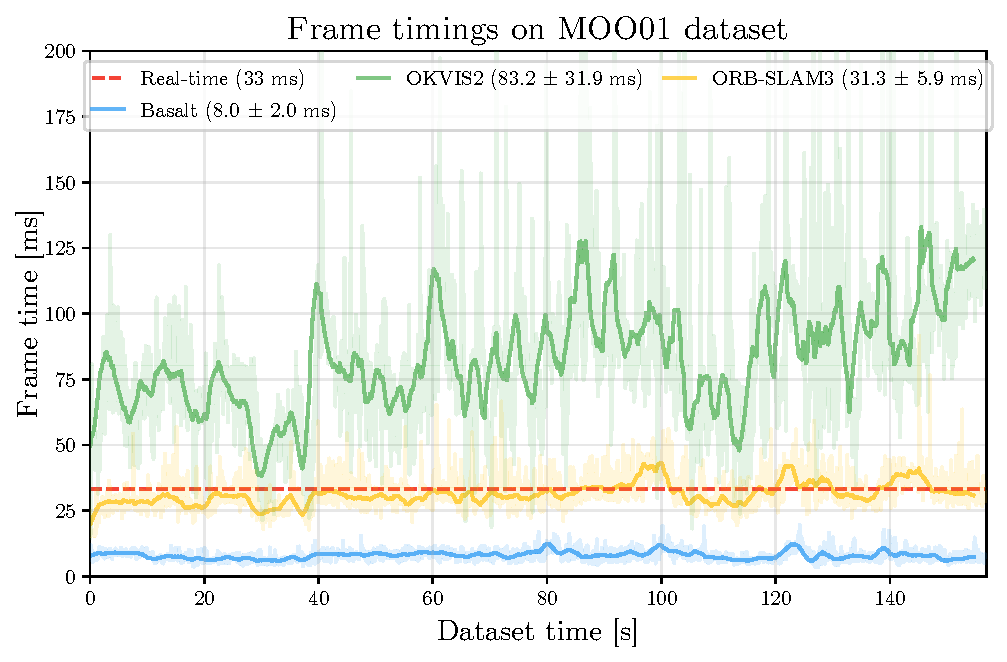
\includegraphics[width=\textwidth]{img/experiments/MOO01.timings.pdf}
        \caption{Secuencia capturada con Odyssey+.}
        \label{fig:msdmo_sota_timings}
    \end{subfigure}
    \hfill
    \begin{subfigure}[b]{0.48\textwidth}
        \centering
        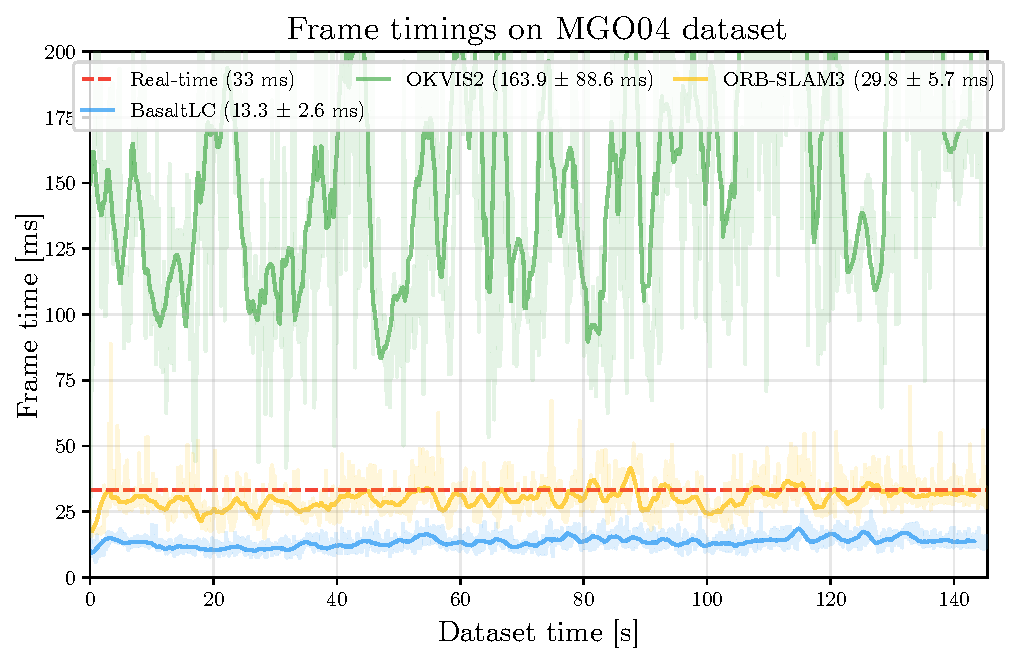
\includegraphics[width=\textwidth]{img/experiments/MGO04.timings.pdf}
        \caption{Secuencia capturada con HP Reverb G2 V2.}
        \label{fig:msdmg_sota_timings}
    \end{subfigure}
    \hfill
    \begin{subfigure}[b]{0.48\textwidth}
        \centering
        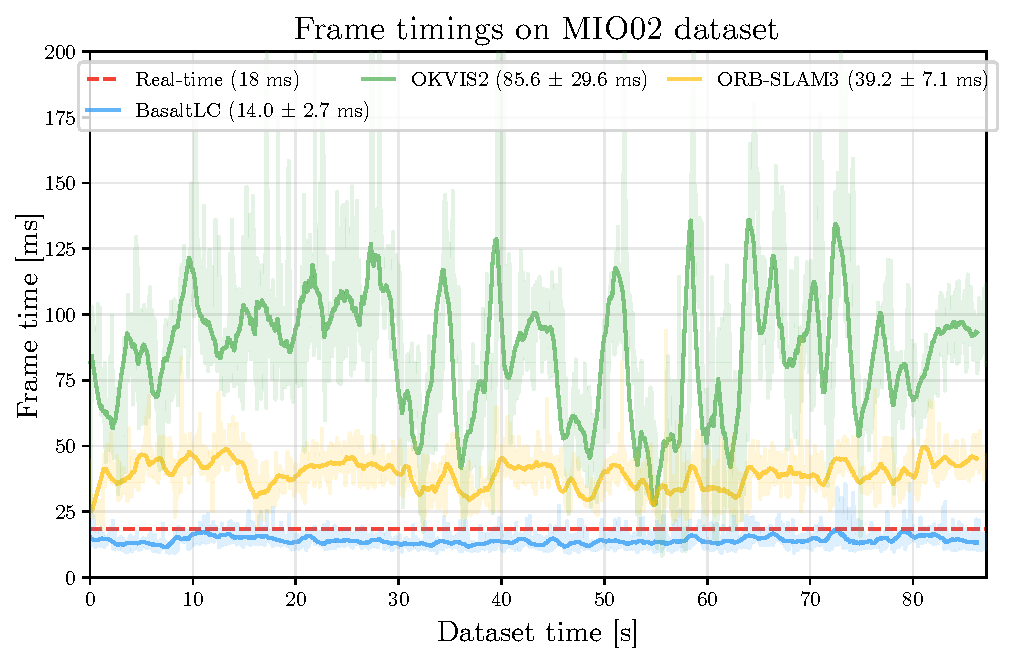
\includegraphics[width=\textwidth]{img/experiments/MIO02.timings.pdf}
        \caption{Secuencia capturada con Valve Index.}
        \label{fig:msdmi_sota_timings}
    \end{subfigure}
    \caption{Tiempo de procesamiento por frame para cada sistema en las secuencias de MO*, MG* y MI* respectivamente.
    Se muestra un promedio móvil con una ventana de 2 segundos (60 frames). En el fondo, los datos sin procesar muestran
    outliers y jitter para cada sistema. Una línea roja marca el límite de tiempo para la operación en tiempo real para cada headset.
    BasaltLC se ejecutó en su versión síncrona, con el mapa asíncrono. Experimento realizado
    en un procesador Intel Core Ultra 9 285H con 32 GB de RAM.}
    \label{fig:msd_sota_timings}
\end{figure}

\section{Análisis de performance de BasaltSLAM}

En esta sección se analiza en detalle la performance de BasaltSLAM, evaluando distintos aspectos clave de su funcionamiento.
En primer lugar, se estudia el comportamiento del sistema en su versión completamente asíncrona, con el objetivo de aprovechar
al máximo su capacidad de procesamiento ejecutando todas las etapas en paralelo. A continuación, se examina cómo el proceso
de culling de keyframes contribuye a mantener estable el tiempo de procesamiento por frame, incluso en trayectorias extensas
de más de 40 minutos. Finalmente, se evalúa el impacto de emplear un método de bundle adjustment numéricamente estable,
como RootBA, que permite ejecutar la optimización en precisión simple.

\subsection{BasaltSLAM en su versión asíncrona}

La Figura \ref{fig:async_timings_basaltslam} muestra el tiempo medio de procesamiento por frame para todas las secuencias
de los distintos datasets. Se observa que en todos los casos el tiempo de procesamiento por frame se mantiene
por debajo del límite para la operación en tiempo real. En las secuencias MI* del headset Valve Index el margen es más ajustado,
pero igualmente se cumple el requisito de tiempo real. En el apéndice X se detallan los tiempos medios de procesamiento
por frame para cada secuencia individual.

\begin{figure}[ht]
    \centering
    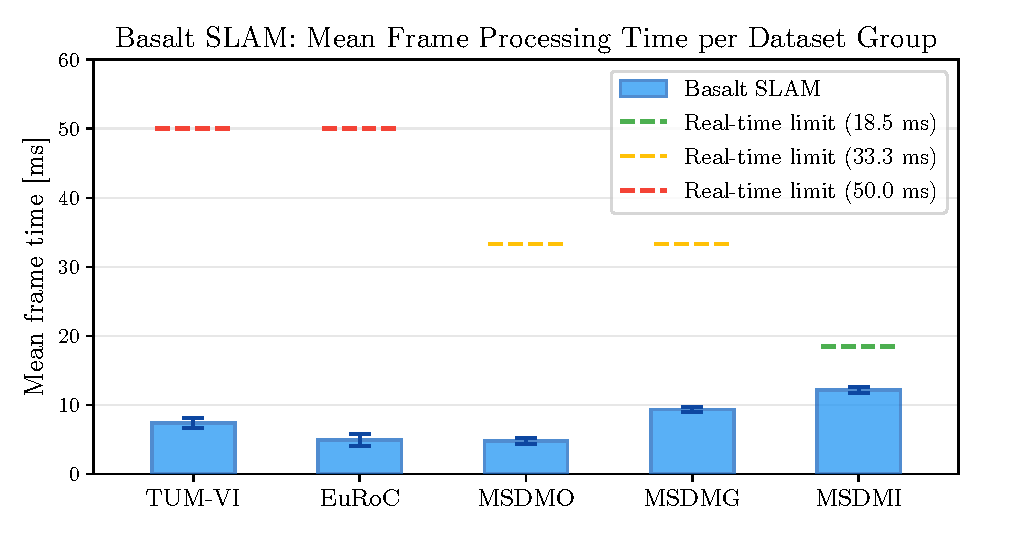
\includegraphics[width=0.8\textwidth]{img/experiments/timings.barplot.pdf}
    \caption{Para cada secuencia, se ejecuta BasaltLC en su versión completamente asíncrona, y se calcula el tiempo medio por frame
    dividiendo el tiempo total por la cantidad de frames. Luego se toma el promedio de estos valores agrupando por tipo de secuencia.
    Se incluye también la varianza en cada tipo de secuencia sobre cada barra.}
    \label{fig:async_timings_basaltslam}
\end{figure}


\subsection{BasaltSLAM en trayectorias extensas}

En esta sección se explica la necesidad de contar con un proceso de culling de keyframes para mantener
un mapa actualizado y un tiempo de procesamiento por frame estable, incluso en trayectorias extensas. Asimismo, se muestra cómo
dicho proceso logra resolver estas limitaciones.

Incluso en una ejecución con el mapa asíncrono, el tiempo de procesamiento por keyframe debe mantenerse estable y por debajo
de cierto límite. De lo contrario, el sistema no podría procesar los keyframes en tiempo real: las colas de
trabajo del mapa se saturarían y se acumularía un retraso que privaría al mapa de la información más reciente.
Esto es especialmente crítico en trayectorias extensas. Para estimar dicho límite, puede considerarse que,
aproximadamente, se selecciona un keyframe cada 7 frames. Por lo tanto, cada keyframe dispone de un intervalo equivalente
a 7 frames para ser procesado en segundo plano, lo que establece un límite aproximado de procesamiento por keyframe
de 7 veces el tiempo máximo permitido por frame. Cabe señalar que este análisis aplica únicamente a las operaciones
ejecutables en segundo plano.

En la Figura \ref{fig:stacked_timings_basaltslam} se muestra el tiempo de procesamiento por keyframe para cada etapa del pipeline
de BasaltSLAM, en su modo síncrono y con culling de keyframes. Se puede observar que el tiempo de procesamiento por keyframe se
mantiene estable, con picos en los momentos en que se detectan o cierran ciclos. En cuanto al tiempo total de ejecución
de la optimización del grafo de poses, se muestra con más detalle en la Figura \ref{fig:pgo_timings_culling}.
Allí, se compara el tiempo total de ejecución de la optimización del grafo de poses para dos versiones de BasaltSLAM: una con
culling de keyframes y otra sin culling de keyframes. En la segunda, el tiempo de ejecución de la optimización del grafo de poses
crece de manera ilimitada. Sin embargo, en la versión que realiza culling de keyframes, el tiempo de optimización del grafo
crece al comienzo, y luego se mantiene estable cerca del límite establecido.

\begin{figure}[ht]
    \centering
    \includegraphics[width=0.8\textwidth]{img/experiments/kftimings.MGO12.pdf}
    \caption{Tiempo de procesamiento por keyframe para la secuencia MGO12. Para cada timestamp se encuentra el tiempo que tomó
    cada etapa del pipeline de BasaltSLAM. Se ejecutó el sistema en su versión síncrona, y es por eso que se observan tiempos
    más altos, con picos en los momentos en que suceden las operaciones más costosas de loop closure.}
    \label{fig:stacked_timings_basaltslam}
\end{figure}

\begin{figure}[ht]
    \centering
    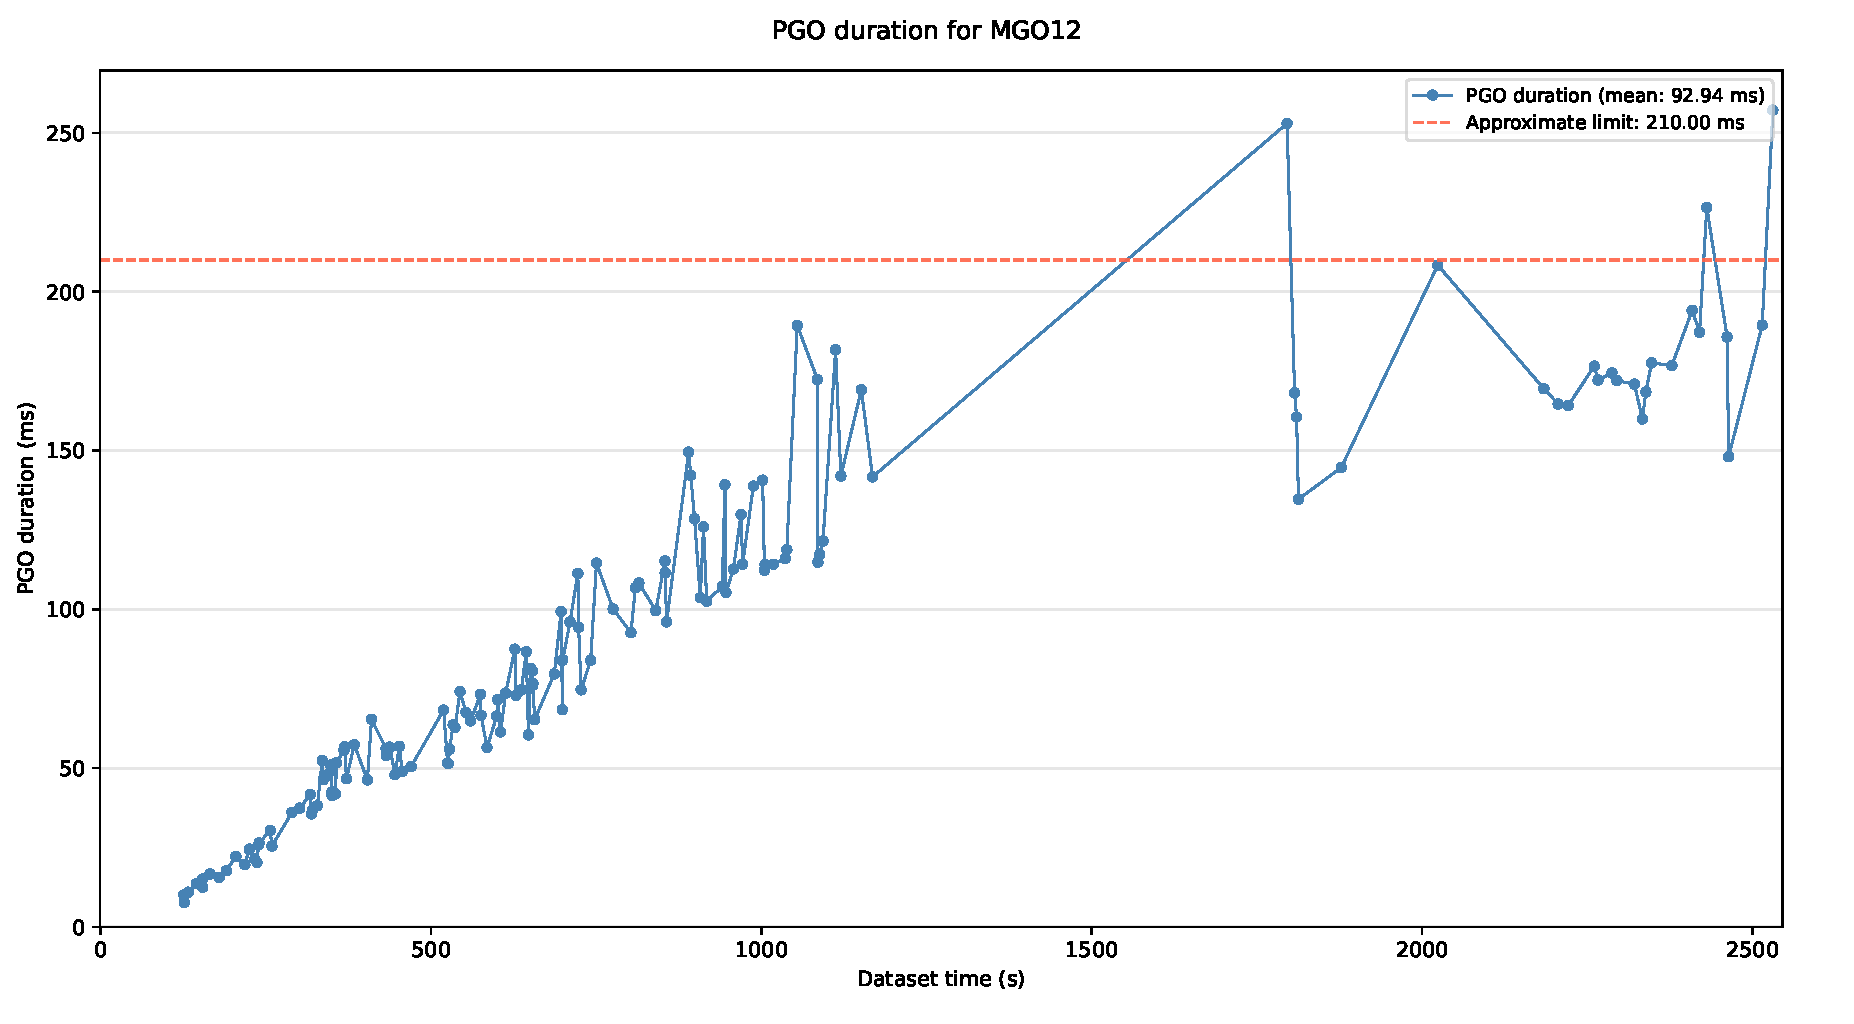
\includegraphics[width=0.8\textwidth]{img/experiments/pgo.timings.MGO12.pdf}
    \caption{Tiempo total de ejecución de la optimización del grafo de poses, para cada cierre de ciclo. Se comparan 
    dos versiones de BasaltSLAM: una con culling de keyframes y otra sin culling de keyframes. La línea punteada roja
    marca el límite aproximado para la operación en tiempo real.}
    \label{fig:pgo_timings_culling}
\end{figure}


\subsection{RootBA: float vs double}

Una de las ventajas de emplear un método como RootBA para la optimización final es su estabilidad numérica, que permite
ejecutar la optimización en precisión simple sin degradar la calidad de la estimación. Esto puede verificarse en el apéndice X,
donde se muestra que los resultados de ATE obtenidos ejecutando RootBA en precisión simple y doble son equivalentes.

En la Figura \ref{fig:rootba_timings} se muestra el tiempo total de ejecución de RootBA en precisión simple y doble para cada secuencia.
Teniendo en cuenta el tiempo total de todas las secuencias de cada dataset, sin subdividir por tipo de secuencia, se obtienen
los siguientes resultados:
en MSD la mediana se reduce en un 50\%; en TUMVI, la mediana se reduce en un 42\%; en Euroc, la mediana se reduce en un 50\%.

En las secuencias de ``Outdoors'' el tiempo de ejecución es elevado. Esto no se debe necesariamente al número de keyframes
u observaciones, sino a que el mapa recibido por RootBA se encuentra mal condicionado. En consecuencia,
el solver carece de un buen precondicionante y requiere más iteraciones para resolver cada sistema de ecuaciones.

\begin{figure}[ht]
    \centering
    \begin{subfigure}[b]{0.8\textwidth}
        \centering
        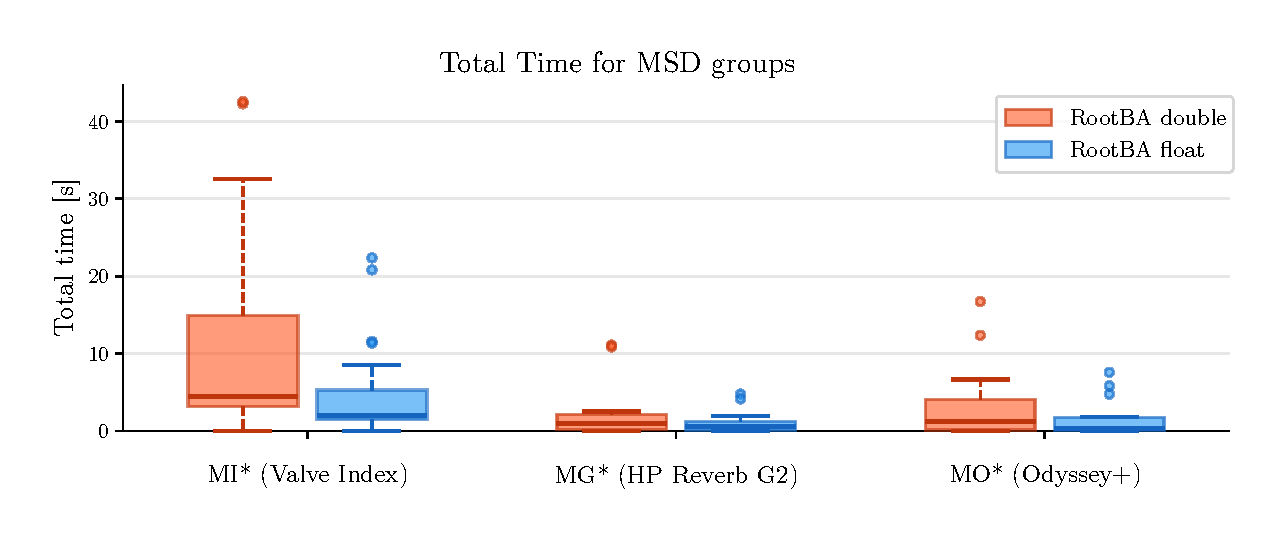
\includegraphics[width=\textwidth]{img/experiments/msd.rootba.times.pdf}
        \caption{Secuencias de MSD.}
        \label{fig:msd_rootba_timings}
    \end{subfigure}
    \hfill
    \begin{subfigure}[b]{0.8\textwidth}
        \centering
        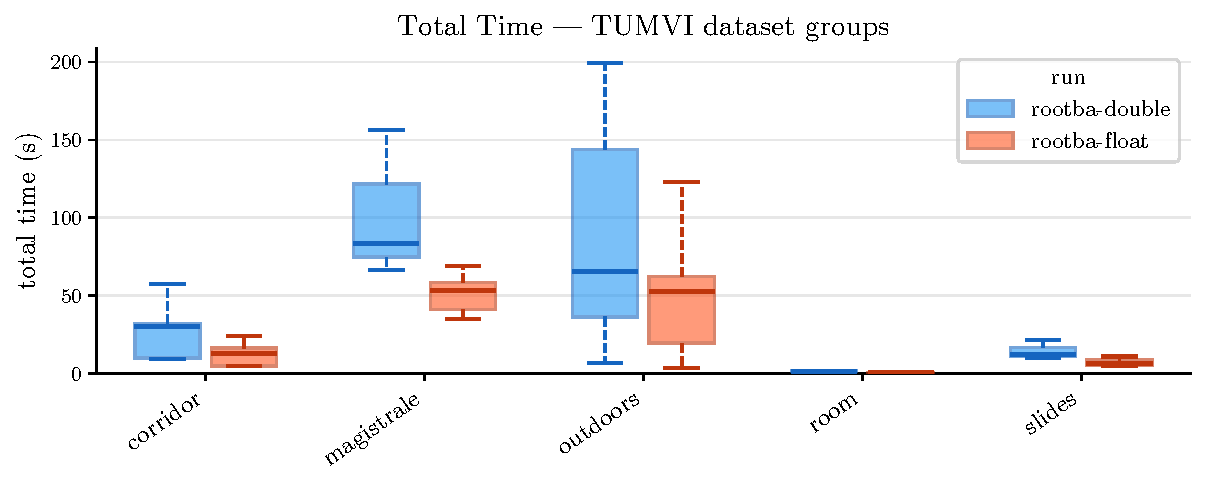
\includegraphics[width=\textwidth]{img/experiments/tumvi.rootba.times.pdf}
        \caption{Secuencias de TUM-VI.}
        \label{fig:tumvi_rootba_timings}
    \end{subfigure}
    \hfill
    \begin{subfigure}[b]{0.8\textwidth}
        \centering
        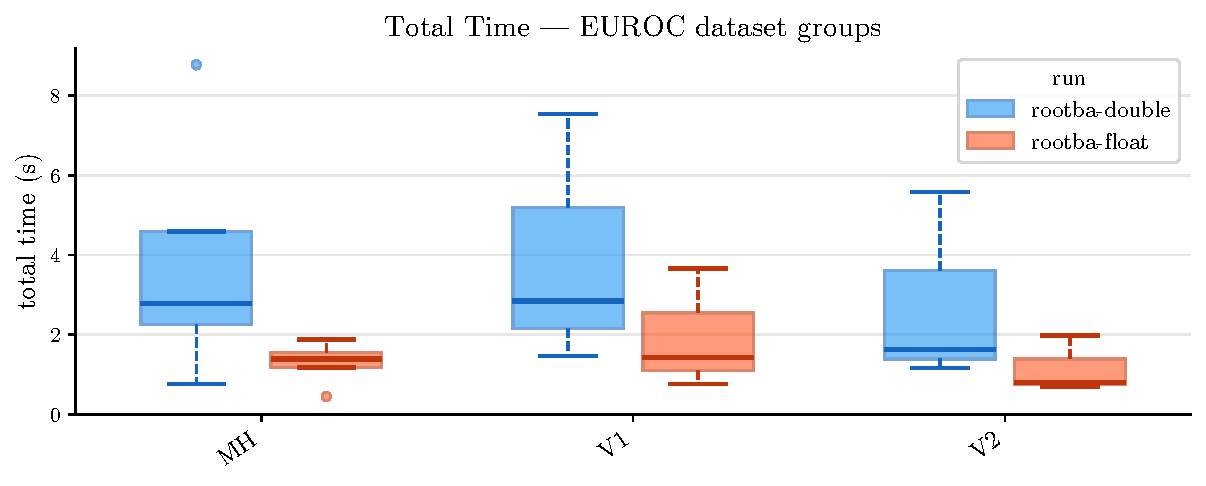
\includegraphics[width=\textwidth]{img/experiments/euroc.rootba.times.pdf}
        \caption{Secuencias de EuRoC.}
        \label{fig:euroc_rootba_timings}
    \end{subfigure}
    \caption{Boxplots de tiempos totales de ejecución de RootBA en precisión simple y doble para cada secuencia.
    Ambas versiones fueron ejecutadas sobre el mismo mapa. Experimento realizado en un procesador Intel Core
    i5-13600 13th Gen con 32 GB de RAM.}
    \label{fig:rootba_timings}
\end{figure}


\section{Discusión} \label{sec:discussion}
